The experiments answer five questions.
\begin{enumerate}[label=(Q\arabic*),leftmargin=*,itemsep=1pt]
\item \emph{Recovery and accuracy.} Does DisCo-CFL recover the concept groups without being told their number, is it more accurate than the alternatives, does it treat small groups fairly, and how robust is it to the strength of the shift, the number of groups, partial participation and scale? We answer this in three groups of experiments (Table~\ref{tab:scenarios}): small CNNs trained from scratch on image datasets with synthetic concept groups (Section~\ref{sec:small}); a pretrained ResNet-18 on natural domain shift and on CIFAR-100, and FEMNIST writers without ground-truth groups with the small CNN (Section~\ref{sec:real}); and four further datasets, including text, that test the scope of the method on data not used to develop it (Section~\ref{sec:extra}).
\item \emph{Failures and theory.} When does DisCo-CFL fail, and does the separation condition of Theorem~\ref{thm:rec} predict it? Section~\ref{sec:sep} relates every outcome to the estimated separation and checks that the results hold under the shrinkage that the theorem covers.
\item \emph{Reference model.} Can the main cause of failure, a reference model that does not yet separate the groups, be removed without labels? Section~\ref{sec:warmup} evaluates a label-free rule for the length of the warm-up.
\item \emph{Beyond accuracy.} What do the explanations and certificates deliver, and how does the clustering behave when the reference model is trained on other clients, when concepts drift, when some clients are malicious and under privacy noise (Section~\ref{sec:fat-exp})?
\item \emph{Design and cost.} Which components matter, how sensitive is the method to its constants, and what does it cost (Section~\ref{sec:sens-cost})?
\end{enumerate}
Section~\ref{sec:setup} describes the benchmarks, the baselines, the metrics and the statistical protocol for all of them.

\subsection{Setup}\label{sec:setup}
\paragraph{Datasets.} We use four image datasets of increasing difficulty: MNIST~\citep{lecun1998mnist}, Fashion-MNIST~\citep{xiao2017fmnist} (the main benchmark), SVHN~\citep{netzer2011svhn} (natural photographs of house numbers) and CIFAR-10~\citep{krizhevsky2009cifar} (natural object images). Section~\ref{sec:real} adds realistic benchmarks with a pretrained ResNet-18: PACS, Office-Home and CIFAR-100. Federations are built from them following the non-IID taxonomy used in the survey~\citep{benali2026survey}, which lists image classification with rotations and label swaps as the standard CFL benchmark~\citep[Table~6]{benali2026survey}.

\paragraph{Heterogeneity.} Each client belongs to a latent concept group. \emph{Concept shift on features} is a rotation of the inputs (by $0^\circ,90^\circ,180^\circ,270^\circ$, or by $0,\theta,2\theta,3\theta$ in the strength sweep). \emph{Concept shift on targets} is a label permutation that swaps two pairs of classes per group. On top of this, every client has \emph{target skew} (Dirichlet label proportions, $\alpha=0.3$, or $\alpha=0.1$ in the label-only scenario) and, where indicated, \emph{quantity skew} (log-normal dataset sizes with $\sigma=1$, clipped to $[30,3200]$, mean 400). Table~\ref{tab:scenarios} lists all scenarios. Each client has a local test set drawn with its own label proportions and transformation. We also evaluate every model on a class-balanced test set of its client's concept (\emph{concept accuracy}), which measures generalisation beyond the local label mix.

\begin{table}[!htbp]
\centering
\caption{Scenarios. $N$: clients; groups: number of concept groups; QS: quantity skew; part.: fraction of clients per round.}\label{tab:scenarios}
\small
\resizebox{\textwidth}{!}{%
\begin{tabular}{llllcl}
\toprule
Scenario & Dataset(s) & Concept groups & $N$ & QS & Other \\
\midrule
Rotation & FMNIST, MNIST, SVHN, CIFAR-10 & 4 rotations ($90^\circ$ steps) & 40 & -- & \\
Label swap & FMNIST, MNIST, SVHN, CIFAR-10 & 4 labelings (2 swapped pairs) & 40 & -- & \\
Rotation + QS & FMNIST & 4 rotations & 40 & \checkmark & \\
Mixed + QS & FMNIST & 2 rotations $\times$ 2 labelings & 40 & \checkmark & \\
Label skew only & FMNIST & 1 (true $K=1$) & 40 & \checkmark & $\alpha=0.1$ \\
Minority groups & FMNIST & 4 rotations, 25/9/4/2 clients & 40 & -- & \\
Strength $\theta$ & FMNIST & 4 rotations, $\theta\in\{15^\circ,30^\circ,45^\circ\}$ & 40 & -- & \\
Groups $K$ & FMNIST & $K\in\{2,4,8\}$ labelings & 40 & -- & \\
Partial participation & FMNIST & rotation / label swap & 40 & -- & part.\ $=0.3$ \\
Scale & FMNIST & 4 rotations & 200 & -- & 200 samples/client \\
\bottomrule
\end{tabular}}
\end{table}

\paragraph{Training.} All methods use the same CNN (two convolutional and two fully connected layers; $d=46{,}730$ parameters for $28\times28$ inputs and $65{,}962$ for $32\times32$ colour images), SGD with learning rate $0.05$, batch size 32, one local epoch per round and 50 communication rounds. Methods with a warm-up (DisCo-CFL, FL+HC, FeSEM, Oracle) spend 10 of the 50 rounds on FedAvg. \emph{Local} trains each client alone for 50 epochs. The six Fashion-MNIST scenarios of Table~\ref{tab:main} and the MNIST, SVHN and CIFAR-10 scenarios are run with five seeds, the sweeps and ablations with three. A seed changes the federation, the initialisation and the sketch. Section~\ref{sec:cost} reports wall-clock time and communication for every method.

\paragraph{Baselines.} We compare with twelve methods that cover all three families of the taxonomy, the three closest class-wise or frozen-model methods, and the main alternatives to clustering:
\begin{itemize}[leftmargin=*,itemsep=1pt]
\item \emph{Single model / personalisation:} FedAvg~\citep{mcmahan2017fedavg}; Local; FedAvg-FT (FedAvg followed by one epoch of local fine-tuning, a standard personalisation baseline).
\item \emph{Client-side:} IFCA~\citep{ghosh2020ifca}.
\item \emph{Server-side:} CFL/MTCFL~\citep{sattler2021cfl} (recursive cosine bipartitioning, triggered when the norm of the aggregated update falls below $\varepsilon_1=0.9$ times the mean client-update norm); FL+HC~\citep{briggs2020flhc} (Ward clustering of local updates after the warm-up); FeSEM~\citep{long2023fesem} (EM-like assignment to the nearest of $K$ centres in parameter space, with the same warm-up and a $k$-means++ initialisation on the clients' local models).
\item \emph{Metadata-based:} PACFL~\citep{vahidian2023pacfl} (principal angles between client data subspaces, $p=3$).
\item \emph{Closest methods}, reimplemented from the papers with the same model, optimiser, data and number of rounds as all other methods: StoCFL~\citep{zeng2025stocfl} (normalised full-batch gradients at the initial model, greedy merging while the cosine exceeds $\tau_{\rm S}=0.5$, bi-level training with a proximal weight $0.05$; two local epochs per round, one for the cluster model and one for the global model); StoCFL-W, the same with the gradients taken at the 10-round warm-up model that DisCo-CFL uses, so that the two differ only in the signal and the rule; FedCCFA~\citep{chen2024fedccfa} (shared feature extractor, per-class clustering of balanced classifier rows by DBSCAN on the MADD distance with radius $0.1$ and one sample per core, classifier averaging within the per-class clusters, and prototype alignment; each client predicts with its personal model, i.e.\ the shared extractor and its classifier after the local classifier epoch of the protocol); and FedDAG-C, the clustering stage of FedDAG~\citep{pramanik2026feddag} (gradient similarity after two local epochs fused with frequency-weighted principal angles between class-wise data subspaces, average linkage with the true $K$, then FedAvg within clusters). FedCCFA clusters each class separately; for ARI we use the partition of clients induced by identical cluster memberships over all classes. The deviations from the original papers (a single SGD optimiser for all methods; for FedDAG-C, a fixed fusion weight instead of its adaptive weighting and the true $K$ instead of an index-based choice) are documented in the code.
\item \emph{Oracle:} FedAvg inside the ground-truth groups (an upper reference).
\end{itemize}
IFCA, FL+HC, FeSEM, PACFL and FedDAG-C are \emph{given the true number of groups} $K$, which favours them. DisCo-CFL, MTCFL, StoCFL and FedCCFA find $K$ on their own. Thresholds of the baselines that find $K$ were selected on the same pilot runs as those of DisCo-CFL: the MTCFL thresholds and FeSEM initialisation in the original study, and, after the correction described below, the StoCFL threshold ($\tau_{\rm S}\in\{0.1,0.3,0.5,0.7,0.8,0.9\}$, at the initial and at the warm-up model) and the FedCCFA radius ($\{0.02,0.05,0.1,0.2,0.4\}$). No StoCFL threshold reaches a mean pilot ARI above $0.1$, so we keep the published default $0.5$; for FedCCFA the published default $0.1$ has the highest mean pilot ARI. \emph{Budgets.} All methods use 50 rounds of one local epoch per client, except StoCFL (two epochs per round) and FedDAG-C (two warm-up epochs); warm-up rounds count towards the 50. Hyperparameters of the baselines were otherwise taken from their papers, without further tuning for any method.

\paragraph{DisCo-CFL.} Sketch dimension $p=1024$, at most 200 samples per class for the signature, classes with fewer than 4 samples not reported, $\tau=0.9$, $\lambda=0.5$, $e_{\min}=0.05$, low-evidence threshold $0.3$, $z=2$, per-sample clipping $C_{\rm clip}=0.5$. These values, and the design choices of bottleneck linkage and evidence-ordered merging, were fixed during pilot runs on seed 0 of the Rotation, Label swap, Mixed + QS and label-only configurations (and seed 1 of Label swap with QS), using clustering quality \emph{measured against the ground-truth groups}, which a deployment would not have. They are kept identical for all scenarios, seeds and datasets. Seeds 1 and 2, the sweeps, and the MNIST, SVHN and CIFAR-10 results were not used for design. Per-sample clipping ($C_{\rm clip}$ chosen on seed 0 only, from $\{0.5,1,2\}$ in all scenarios and additionally $\{0.1,0.25\}$ in the label-only scenario) was added after a first sensitivity study showed over-splitting caused by heavy-tailed per-sample gradients. The run without clipping is reported as an ablation. \emph{Correction and re-selection of the threshold.} After submission we found an implementation error in the training primitive shared by all methods: a model vector passed to several clients in the same round was modified in place, so that clients of the same cluster effectively trained one after another instead of in parallel. This affected every method and every result of the original manuscript. All experiments reported here were rerun with the corrected code. With the corrected code the threshold $\tau=0.8$ merged groups on the pilot runs (ARI $0.60$ on Rotation and $0.64$ on Mixed + QS), and we re-selected it on the same pilot runs (seed 0 of the four configurations, $\tau\in\{0.70,0.75,0.80,0.85,0.90\}$, $T_0\in\{10,20,30\}$). $\tau=0.9$ with $T_0=10$ gives ARI $0.93$, $1.00$, $1.00$ and $1.00$ and was adopted; the other constants were not changed. \emph{Development and evaluation runs.} The pilot runs (seed 0 of Rotation, Label swap, Mixed + QS and label-only, and seed 0 of PACS for the learning rate of Section~\ref{sec:real}) are development runs. We report every result both on all runs and on the held-out runs only, which exclude them. On the colour datasets we also report DisCo-T30, which uses 30 warm-up rounds (Section~\ref{sec:datasets}). Section~\ref{sec:sens} reports the sensitivity to $\tau$ and $\lambda$.

\paragraph{Metrics.} \emph{Performance:} mean local test accuracy (Acc), with the prior correction of Section~\ref{sec:pc} applied identically to every method, and concept accuracy. \emph{Fairness:} accuracy of the worst 10\% of clients (Acc@10\%), accuracy of the worst concept group (Worst-grp), Jain's index. \emph{Clustering:} ARI with respect to the groups, number of clusters $K$, and the \emph{conflict-merge rate}: the fraction of conflicting client pairs (Definition~\ref{def:concept}) that end up in the same cluster. ARI penalises the legitimate placement of compatible clients (e.g.\ a client of a label-swap group that holds none of the swapped classes), whereas the conflict-merge rate measures exactly the harmful errors. \emph{Statistics.} Runs with different seeds of the same scenario share the scenario, so (scenario, seed) pairs are not independent. We report, per dataset, means with 95\% $t$-intervals over seeds and \emph{failure rates} (fraction of runs with ARI below $0.5$ when there are several groups). For comparisons across scenarios we use (i) a hierarchical bootstrap that resamples scenarios and then seeds within scenarios~\citep{saravanan2020hierarchical} ($10^4$ replicates) for the mean difference between DisCo-CFL and each baseline, and (ii) one-sided Wilcoxon signed-rank tests on scenario-level means, one value per scenario~\citep{demsar2006statistical}. Both are reported on all runs and on held-out runs.

\subsection{Small CNNs: performance, fairness and clustering quality}\label{sec:small}
\paragraph{Main results.}
Table~\ref{tab:main} reports Fashion-MNIST results for all methods with five seeds: means with 95\% $t$-intervals over seeds. Accuracy is \emph{with} the prior correction~\eqref{eq:pc}, applied identically to every method. Table~\ref{tab:failure} gives failure rates, Table~\ref{tab:hier} the hierarchical comparison over scenarios, and Table~\ref{tab:diag} the separation and coverage diagnostics of Section~\ref{sec:theory} for every scenario.

\begin{table}[!htbp]
\centering
\caption{Fashion-MNIST, 40 clients, 5 seeds: mean $\pm$ half-width of the 95\% $t$-interval over seeds. Acc: mean local accuracy with prior correction. Concept: accuracy on the class-balanced test set of the client's concept. Worst-grp: accuracy of the worst concept group. Conflict: fraction of conflicting client pairs placed in one cluster (merge and attachment stages combined). IFCA, FeSEM, FL+HC, PACFL and FedDAG-C receive the true $K$ (in \emph{Label skew only}, $K=1$); DisCo-CFL, MTCFL, StoCFL and FedCCFA find it. For FedCCFA, ARI and $K$ refer to the client partition induced by its per-class clusters.}\label{tab:main}
{\scriptsize
\begin{tabular}{l r c c c c c c}
\toprule
Method & n & Acc (\%) & Concept (\%) & Worst-grp (\%) & ARI & K & Conflict (\%) \\
\midrule
\multicolumn{8}{l}{\textit{Rotation}} \\
DisCo & 5 & 89.1 $\pm$ 1.1 & 76.4 $\pm$ 1.0 & 87.4 $\pm$ 1.7 & 0.92 $\pm$ 0.06 & 4.4 & 1.1 \\
DisCo-noAttach & 5 & 89.1 $\pm$ 1.1 & 76.2 $\pm$ 1.0 & 87.3 $\pm$ 1.6 & 0.91 $\pm$ 0.07 & 4.8 & 1.1 \\
FedAvg & 5 & 82.4 $\pm$ 1.2 & 65.4 $\pm$ 1.1 & 80.7 $\pm$ 2.1 & 0.00 $\pm$ 0.00 & 1.0 & 100.0 \\
Local & 5 & 87.4 $\pm$ 0.9 & 54.0 $\pm$ 2.4 & 85.2 $\pm$ 1.5 & 0.00 $\pm$ 0.00 & 40.0 & 0.0 \\
FedAvg-FT & 5 & 83.7 $\pm$ 1.8 & 64.8 $\pm$ 1.3 & 81.5 $\pm$ 3.2 & 0.00 $\pm$ 0.00 & 40.0 & 0.0 \\
IFCA & 5 & 86.2 $\pm$ 1.9 & 66.9 $\pm$ 4.8 & 84.2 $\pm$ 2.8 & 0.27 $\pm$ 0.21 & 4.0 & 23.6 \\
FeSEM & 5 & 87.4 $\pm$ 1.7 & 70.8 $\pm$ 3.4 & 85.8 $\pm$ 1.5 & 0.43 $\pm$ 0.28 & 4.0 & 24.7 \\
MTCFL & 5 & 88.1 $\pm$ 1.3 & 64.1 $\pm$ 2.2 & 86.8 $\pm$ 1.5 & 0.11 $\pm$ 0.02 & 24.2 & 0.3 \\
FL+HC & 5 & 88.4 $\pm$ 0.9 & 74.3 $\pm$ 2.2 & 86.9 $\pm$ 0.8 & 0.70 $\pm$ 0.18 & 4.0 & 9.3 \\
PACFL & 5 & 87.5 $\pm$ 1.6 & 72.0 $\pm$ 1.0 & 85.2 $\pm$ 2.2 & 0.47 $\pm$ 0.09 & 4.0 & 20.6 \\
StoCFL & 5 & 85.3 $\pm$ 1.6 & 61.2 $\pm$ 1.5 & 83.1 $\pm$ 1.4 & 0.03 $\pm$ 0.06 & 12.6 & 8.6 \\
StoCFL-W & 5 & 86.7 $\pm$ 1.3 & 64.8 $\pm$ 2.1 & 84.9 $\pm$ 1.4 & 0.10 $\pm$ 0.05 & 16.2 & 3.9 \\
FedCCFA & 5 & 83.3 $\pm$ 0.9 & 62.5 $\pm$ 1.4 & 80.2 $\pm$ 1.1 & 0.00 $\pm$ 0.00 & 1.2 & 99.0 \\
FedDAG-C & 5 & 88.6 $\pm$ 0.7 & 74.2 $\pm$ 3.4 & 86.6 $\pm$ 1.7 & 0.69 $\pm$ 0.26 & 4.0 & 12.1 \\
Oracle & 5 & 89.3 $\pm$ 1.0 & 77.4 $\pm$ 0.7 & 87.6 $\pm$ 1.6 & 1.00 $\pm$ 0.00 & 4.0 & 0.0 \\
\addlinespace
\multicolumn{8}{l}{\textit{Label swap}} \\
DisCo & 5 & 89.2 $\pm$ 0.9 & 76.7 $\pm$ 0.8 & 87.7 $\pm$ 1.1 & 0.97 $\pm$ 0.05 & 4.0 & 0.0 \\
DisCo-noAttach & 5 & 89.2 $\pm$ 0.9 & 76.5 $\pm$ 1.0 & 87.7 $\pm$ 1.1 & 0.97 $\pm$ 0.04 & 4.2 & 0.0 \\
FedAvg & 5 & 74.7 $\pm$ 2.7 & 53.3 $\pm$ 0.5 & 67.1 $\pm$ 6.7 & 0.00 $\pm$ 0.00 & 1.0 & 100.0 \\
Local & 5 & 87.3 $\pm$ 1.0 & 54.2 $\pm$ 2.3 & 85.3 $\pm$ 1.3 & 0.00 $\pm$ 0.00 & 40.0 & 0.0 \\
FedAvg-FT & 5 & 85.5 $\pm$ 2.2 & 66.3 $\pm$ 1.5 & 83.4 $\pm$ 2.8 & 0.00 $\pm$ 0.00 & 40.0 & 0.0 \\
IFCA & 5 & 84.5 $\pm$ 1.9 & 61.2 $\pm$ 7.2 & 82.1 $\pm$ 2.7 & 0.30 $\pm$ 0.15 & 4.0 & 19.7 \\
FeSEM & 5 & 85.8 $\pm$ 1.7 & 64.8 $\pm$ 5.8 & 81.3 $\pm$ 4.6 & 0.39 $\pm$ 0.13 & 4.0 & 17.9 \\
MTCFL & 5 & 88.1 $\pm$ 1.3 & 64.4 $\pm$ 2.8 & 86.2 $\pm$ 1.1 & 0.11 $\pm$ 0.02 & 24.2 & 0.1 \\
FL+HC & 5 & 88.3 $\pm$ 0.9 & 72.6 $\pm$ 4.4 & 86.5 $\pm$ 2.0 & 0.69 $\pm$ 0.31 & 4.0 & 7.7 \\
PACFL & 5 & 76.8 $\pm$ 3.9 & 50.6 $\pm$ 1.3 & 70.5 $\pm$ 5.2 & $-$0.02 $\pm$ 0.02 & 4.0 & 35.1 \\
StoCFL & 5 & 81.3 $\pm$ 2.7 & 53.2 $\pm$ 1.8 & 74.9 $\pm$ 6.8 & 0.01 $\pm$ 0.04 & 11.4 & 9.5 \\
StoCFL-W & 5 & 86.8 $\pm$ 1.5 & 64.1 $\pm$ 2.6 & 85.0 $\pm$ 1.0 & 0.15 $\pm$ 0.04 & 16.4 & 3.2 \\
FedCCFA & 5 & 85.7 $\pm$ 0.7 & 64.3 $\pm$ 1.5 & 82.4 $\pm$ 2.3 & 0.00 $\pm$ 0.00 & 2.4 & 92.7 \\
FedDAG-C & 5 & 84.2 $\pm$ 2.9 & 61.7 $\pm$ 4.3 & 80.6 $\pm$ 3.9 & 0.37 $\pm$ 0.14 & 4.0 & 21.1 \\
Oracle & 5 & 89.2 $\pm$ 1.0 & 77.0 $\pm$ 0.8 & 87.7 $\pm$ 1.3 & 1.00 $\pm$ 0.00 & 4.0 & 0.0 \\
\addlinespace
\multicolumn{8}{l}{\textit{Rotation + QS}} \\
DisCo & 5 & 88.9 $\pm$ 2.5 & 76.4 $\pm$ 1.5 & 86.5 $\pm$ 4.0 & 0.99 $\pm$ 0.03 & 4.2 & 0.0 \\
DisCo-noAttach & 5 & 88.8 $\pm$ 2.4 & 76.1 $\pm$ 1.6 & 86.2 $\pm$ 3.5 & 0.97 $\pm$ 0.05 & 4.8 & 0.0 \\
FedAvg & 5 & 81.6 $\pm$ 4.2 & 62.7 $\pm$ 4.5 & 75.3 $\pm$ 10.0 & 0.00 $\pm$ 0.00 & 1.0 & 100.0 \\
Local & 5 & 85.3 $\pm$ 2.7 & 51.9 $\pm$ 2.0 & 81.8 $\pm$ 5.3 & 0.00 $\pm$ 0.00 & 40.0 & 0.0 \\
FedAvg-FT & 5 & 82.2 $\pm$ 1.7 & 62.8 $\pm$ 2.6 & 77.9 $\pm$ 4.0 & 0.00 $\pm$ 0.00 & 40.0 & 0.0 \\
IFCA & 5 & 87.6 $\pm$ 2.1 & 71.5 $\pm$ 1.9 & 84.5 $\pm$ 3.9 & 0.54 $\pm$ 0.19 & 3.8 & 17.7 \\
FeSEM & 5 & 83.0 $\pm$ 2.1 & 64.3 $\pm$ 4.4 & 76.7 $\pm$ 5.2 & 0.22 $\pm$ 0.18 & 4.0 & 36.8 \\
MTCFL & 5 & 87.0 $\pm$ 2.4 & 63.4 $\pm$ 2.2 & 84.1 $\pm$ 4.1 & 0.11 $\pm$ 0.01 & 24.8 & 0.2 \\
FL+HC & 5 & 86.5 $\pm$ 2.7 & 71.2 $\pm$ 2.7 & 83.6 $\pm$ 2.7 & 0.56 $\pm$ 0.22 & 4.0 & 17.6 \\
PACFL & 5 & 85.8 $\pm$ 3.8 & 69.7 $\pm$ 5.5 & 81.4 $\pm$ 7.3 & 0.44 $\pm$ 0.05 & 4.0 & 21.9 \\
StoCFL & 5 & 83.5 $\pm$ 1.7 & 59.4 $\pm$ 2.4 & 80.7 $\pm$ 2.8 & 0.05 $\pm$ 0.07 & 14.0 & 7.4 \\
StoCFL-W & 5 & 85.8 $\pm$ 2.8 & 65.0 $\pm$ 2.5 & 82.6 $\pm$ 4.8 & 0.17 $\pm$ 0.09 & 17.2 & 3.7 \\
FedCCFA & 5 & 83.4 $\pm$ 3.4 & 61.0 $\pm$ 2.6 & 78.8 $\pm$ 8.3 & 0.00 $\pm$ 0.00 & 1.2 & 99.0 \\
FedDAG-C & 5 & 86.3 $\pm$ 2.8 & 69.1 $\pm$ 1.8 & 82.5 $\pm$ 5.2 & 0.44 $\pm$ 0.07 & 4.0 & 19.6 \\
Oracle & 5 & 88.9 $\pm$ 2.5 & 76.7 $\pm$ 2.0 & 86.6 $\pm$ 4.0 & 1.00 $\pm$ 0.00 & 4.0 & 0.0 \\
\addlinespace
\bottomrule
\end{tabular}
}


\end{table}

\begin{table}[!htbp]
\centering
\caption*{Table~\ref{tab:main} (continued).}
{\scriptsize
\begin{tabular}{l r c c c c c c}
\toprule
Method & n & Acc (\%) & Concept (\%) & Worst-grp (\%) & ARI & K & Conflict (\%) \\
\midrule
\multicolumn{8}{l}{\textit{Mixed + QS}} \\
DisCo & 5 & 89.0 $\pm$ 2.6 & 76.4 $\pm$ 1.3 & 86.7 $\pm$ 4.1 & 0.96 $\pm$ 0.07 & 4.2 & 0.0 \\
DisCo-noAttach & 5 & 89.0 $\pm$ 2.5 & 76.2 $\pm$ 1.5 & 86.7 $\pm$ 3.9 & 0.96 $\pm$ 0.07 & 4.4 & 0.0 \\
FedAvg & 5 & 81.8 $\pm$ 3.4 & 61.3 $\pm$ 1.3 & 75.0 $\pm$ 6.8 & 0.00 $\pm$ 0.00 & 1.0 & 100.0 \\
Local & 5 & 85.4 $\pm$ 2.8 & 51.8 $\pm$ 1.7 & 81.9 $\pm$ 4.8 & 0.00 $\pm$ 0.00 & 40.0 & 0.0 \\
FedAvg-FT & 5 & 84.0 $\pm$ 1.1 & 66.2 $\pm$ 1.6 & 81.1 $\pm$ 1.7 & 0.00 $\pm$ 0.00 & 40.0 & 0.0 \\
IFCA & 5 & 87.6 $\pm$ 2.1 & 71.2 $\pm$ 0.7 & 85.0 $\pm$ 4.0 & 0.49 $\pm$ 0.09 & 3.6 & 23.3 \\
FeSEM & 5 & 83.3 $\pm$ 2.0 & 63.5 $\pm$ 2.9 & 76.9 $\pm$ 3.3 & 0.11 $\pm$ 0.09 & 4.0 & 40.3 \\
MTCFL & 5 & 87.7 $\pm$ 1.6 & 63.4 $\pm$ 2.3 & 85.7 $\pm$ 2.6 & 0.08 $\pm$ 0.03 & 25.6 & 0.6 \\
FL+HC & 5 & 84.8 $\pm$ 4.0 & 66.8 $\pm$ 1.8 & 80.6 $\pm$ 6.4 & 0.24 $\pm$ 0.13 & 4.0 & 30.3 \\
PACFL & 5 & 82.5 $\pm$ 3.3 & 61.2 $\pm$ 2.4 & 78.6 $\pm$ 4.2 & 0.19 $\pm$ 0.12 & 4.0 & 22.8 \\
StoCFL & 5 & 83.1 $\pm$ 2.2 & 61.1 $\pm$ 1.4 & 79.2 $\pm$ 3.2 & 0.03 $\pm$ 0.06 & 12.2 & 8.6 \\
StoCFL-W & 5 & 85.3 $\pm$ 2.2 & 63.5 $\pm$ 1.5 & 81.0 $\pm$ 4.3 & 0.08 $\pm$ 0.06 & 14.8 & 5.7 \\
FedCCFA & 5 & 85.6 $\pm$ 2.3 & 65.5 $\pm$ 2.1 & 81.8 $\pm$ 3.5 & 0.00 $\pm$ 0.00 & 1.2 & 98.9 \\
FedDAG-C & 5 & 82.2 $\pm$ 3.0 & 60.1 $\pm$ 2.4 & 77.4 $\pm$ 3.3 & 0.20 $\pm$ 0.20 & 4.0 & 31.9 \\
Oracle & 5 & 89.1 $\pm$ 2.4 & 76.8 $\pm$ 1.7 & 86.7 $\pm$ 4.1 & 1.00 $\pm$ 0.00 & 4.0 & 0.0 \\
\addlinespace
\multicolumn{8}{l}{\textit{Label skew only}} \\
DisCo & 5 & 94.5 $\pm$ 1.0 & 76.7 $\pm$ 2.0 & 94.5 $\pm$ 1.0 & 1.00 $\pm$ 0.00 & 1.0 & 0.0 \\
DisCo-noAttach & 5 & 94.5 $\pm$ 1.0 & 76.5 $\pm$ 1.5 & 94.5 $\pm$ 1.0 & 0.80 $\pm$ 0.56 & 1.2 & 0.0 \\
FedAvg & 5 & 94.5 $\pm$ 1.0 & 76.7 $\pm$ 2.0 & 94.5 $\pm$ 1.0 & 1.00 $\pm$ 0.00 & 1.0 & 0.0 \\
Local & 5 & 92.4 $\pm$ 2.2 & 35.4 $\pm$ 0.9 & 92.4 $\pm$ 2.2 & 0.00 $\pm$ 0.00 & 40.0 & 0.0 \\
FedAvg-FT & 5 & 91.6 $\pm$ 2.0 & 71.0 $\pm$ 2.1 & 91.6 $\pm$ 2.0 & 0.00 $\pm$ 0.00 & 40.0 & 0.0 \\
IFCA & 5 & 94.5 $\pm$ 1.2 & 76.4 $\pm$ 2.0 & 94.5 $\pm$ 1.2 & 1.00 $\pm$ 0.00 & 1.0 & 0.0 \\
FeSEM & 5 & 94.6 $\pm$ 1.0 & 76.7 $\pm$ 2.2 & 94.6 $\pm$ 1.0 & 1.00 $\pm$ 0.00 & 1.0 & 0.0 \\
MTCFL & 5 & 93.7 $\pm$ 1.2 & 54.8 $\pm$ 4.5 & 93.7 $\pm$ 1.2 & 0.00 $\pm$ 0.00 & 26.4 & 0.0 \\
FL+HC & 5 & 94.5 $\pm$ 1.0 & 76.6 $\pm$ 1.9 & 94.5 $\pm$ 1.0 & 1.00 $\pm$ 0.00 & 1.0 & 0.0 \\
PACFL & 5 & 94.5 $\pm$ 1.0 & 76.7 $\pm$ 2.0 & 94.5 $\pm$ 1.0 & 1.00 $\pm$ 0.00 & 1.0 & 0.0 \\
StoCFL & 5 & 93.5 $\pm$ 1.4 & 68.6 $\pm$ 1.6 & 93.5 $\pm$ 1.4 & 0.00 $\pm$ 0.00 & 9.6 & 0.0 \\
StoCFL-W & 5 & 93.4 $\pm$ 1.1 & 70.7 $\pm$ 2.0 & 93.4 $\pm$ 1.1 & 0.00 $\pm$ 0.00 & 9.4 & 0.0 \\
FedCCFA & 5 & 93.1 $\pm$ 1.5 & 71.9 $\pm$ 2.5 & 93.1 $\pm$ 1.5 & 1.00 $\pm$ 0.00 & 1.0 & 0.0 \\
FedDAG-C & 5 & 94.5 $\pm$ 1.1 & 76.7 $\pm$ 1.9 & 94.5 $\pm$ 1.1 & 1.00 $\pm$ 0.00 & 1.0 & 0.0 \\
Oracle & 5 & 94.5 $\pm$ 1.0 & 76.7 $\pm$ 2.0 & 94.5 $\pm$ 1.0 & 1.00 $\pm$ 0.00 & 1.0 & 0.0 \\
\addlinespace
\multicolumn{8}{l}{\textit{Minority groups}} \\
DisCo & 5 & 89.2 $\pm$ 0.9 & 77.2 $\pm$ 1.2 & 87.2 $\pm$ 1.0 & 0.99 $\pm$ 0.01 & 4.0 & 0.1 \\
DisCo-noAttach & 5 & 89.2 $\pm$ 0.9 & 77.1 $\pm$ 1.4 & 87.1 $\pm$ 0.8 & 0.97 $\pm$ 0.07 & 4.6 & 0.0 \\
FedAvg & 5 & 83.4 $\pm$ 1.2 & 67.0 $\pm$ 0.8 & 67.5 $\pm$ 11.8 & 0.00 $\pm$ 0.00 & 1.0 & 100.0 \\
Local & 5 & 87.5 $\pm$ 0.9 & 54.2 $\pm$ 2.3 & 86.0 $\pm$ 1.2 & 0.00 $\pm$ 0.00 & 40.0 & 0.0 \\
FedAvg-FT & 5 & 85.0 $\pm$ 1.9 & 66.9 $\pm$ 0.6 & 78.8 $\pm$ 5.7 & 0.00 $\pm$ 0.00 & 40.0 & 0.0 \\
IFCA & 5 & 87.0 $\pm$ 1.2 & 70.0 $\pm$ 4.1 & 81.2 $\pm$ 3.4 & 0.37 $\pm$ 0.31 & 4.0 & 17.8 \\
FeSEM & 5 & 87.7 $\pm$ 1.9 & 72.2 $\pm$ 3.1 & 80.9 $\pm$ 7.8 & 0.47 $\pm$ 0.32 & 4.0 & 14.7 \\
MTCFL & 5 & 88.3 $\pm$ 0.8 & 65.7 $\pm$ 1.1 & 85.7 $\pm$ 2.2 & 0.05 $\pm$ 0.01 & 24.4 & 0.1 \\
FL+HC & 5 & 88.6 $\pm$ 1.4 & 74.4 $\pm$ 0.8 & 83.8 $\pm$ 2.1 & 0.66 $\pm$ 0.20 & 4.0 & 8.6 \\
PACFL & 5 & 88.0 $\pm$ 0.8 & 72.6 $\pm$ 1.8 & 84.2 $\pm$ 1.2 & 0.45 $\pm$ 0.07 & 4.0 & 18.3 \\
StoCFL & 5 & 86.5 $\pm$ 1.3 & 65.4 $\pm$ 0.8 & 83.3 $\pm$ 1.7 & 0.03 $\pm$ 0.05 & 12.4 & 8.3 \\
StoCFL-W & 5 & 87.4 $\pm$ 0.8 & 67.8 $\pm$ 1.3 & 84.6 $\pm$ 1.9 & 0.07 $\pm$ 0.02 & 15.6 & 3.6 \\
FedCCFA & 5 & 84.7 $\pm$ 1.5 & 64.9 $\pm$ 1.0 & 75.5 $\pm$ 8.8 & 0.01 $\pm$ 0.04 & 1.2 & 98.3 \\
FedDAG-C & 5 & 88.5 $\pm$ 1.0 & 74.1 $\pm$ 2.4 & 84.1 $\pm$ 3.6 & 0.68 $\pm$ 0.27 & 4.0 & 11.7 \\
Oracle & 5 & 89.3 $\pm$ 0.8 & 77.3 $\pm$ 1.2 & 87.4 $\pm$ 1.0 & 1.00 $\pm$ 0.00 & 4.0 & 0.0 \\
\bottomrule
\end{tabular}
}


\end{table}

\paragraph{Recovery of the concept groups (H2).} In all six Fashion-MNIST scenarios DisCo-CFL recovers the groups without being told $K$: mean ARI $0.92$--$1.00$, at most $1.1\%$ of the conflicting pairs merged, and no run with ARI below $0.5$ (Table~\ref{tab:failure}). The weakest scenario is \emph{Rotation} (ARI $0.92\pm0.06$, $K=4.4$): the $0^\circ$ and $180^\circ$ groups are close on the nearly symmetric classes, and some clients that hold mostly such classes are split off or merged. The diagnostics agree with the assumptions of Theorem~\ref{thm:rec}: the estimated separation is $\hat\Delta=0.44$--$0.61$, well above $1-\tau=0.1$, and $98$--$100\%$ of the conflicting pairs share a discriminative class (Table~\ref{tab:diag}). Accuracy and worst-group accuracy are within $0.2$ points of the Oracle in every scenario, and concept accuracy within $1.0$ point.

The baselines that are given the true $K$ merge many conflicting pairs: IFCA 18--24\%, FeSEM 15--40\%, PACFL 18--35\%, FedDAG-C 12--32\% and FL+HC 8--30\%, and they fail (ARI $<0.5$) in 36--88\% of the runs. The closest methods do not recover the groups either. StoCFL compares whole-model gradients at the initial model and fragments the federation into 11--14 clusters with ARI at most $0.05$; with gradients at the warm-up model (StoCFL-W) it forms 15--17 clusters, ARI $\le0.17$. The raw gradient mixes the concept with each client's label mix, exactly the entanglement that the class-conditional signature removes. FedCCFA clusters the classifier of each class separately; its per-class clusters rarely differ between concept groups at the published radius, so the induced partition is almost a single cluster (ARI $0.00$) and its accuracy is 3--6 points below DisCo-CFL. FedDAG-C, which also compares clients class by class but uses data subspaces and gradient angles, is the strongest new baseline on \emph{Rotation} (ARI $0.69$) and much weaker on label swaps (ARI $0.37$), where the data subspaces do not change.

\paragraph{Label skew does not create clusters (H1).} With a single concept and strong target and quantity skew (\emph{Label skew only}), DisCo-CFL returns $K=1$ in all five seeds, and its accuracy equals FedAvg's. MTCFL splits the federation into 26 clusters, StoCFL and StoCFL-W into 9--10, and their concept accuracy drops by 6--22 points. The baselines that receive $K$ are given $K=1$ here, so their single cluster is not a decision.

\paragraph{Performance.} DisCo-CFL is within the confidence interval of the Oracle in every Fashion-MNIST scenario. Its mean accuracy is the highest of all non-oracle methods in the five concept-shift scenarios; in \emph{Label skew only} it equals FedAvg's, and FeSEM is $0.1$ points higher. The margins over the strongest baseline are small on local accuracy (0.5--1.3 points against FedDAG-C, FL+HC, IFCA or MTCFL) and larger on concept accuracy (2.1--5.2 points). Methods that fragment the federation (Local, FedAvg-FT, MTCFL) obtain competitive \emph{local} accuracy, because local test sets share the client's label mix, but their concept accuracy is 10--22 points lower: their models do not generalise to the rest of the client's concept. Across all small-CNN scenarios, including the SVHN and CIFAR-10 failures, the hierarchical bootstrap gives DisCo-CFL a positive mean difference in accuracy against every baseline (Table~\ref{tab:hier}). The 95\% interval excludes zero except against Local ($+0.6$, $[-1.8,+2.5]$) and MTCFL ($+0.9$, $[-0.6,+2.2]$), the two methods that fit each client's label mix; the closest baseline with an interval that excludes zero is FL+HC ($+1.1$, $[+0.3,+1.8]$). On concept accuracy every interval excludes zero ($+4.7$ to $+20.5$ points). These differences are averages over scenarios in which DisCo-CFL succeeds and scenarios in which it fails, and the per-dataset tables are the more informative summary. The Wilcoxon test on scenario-level means can be significant where the bootstrap interval includes zero (MTCFL: $p=0.007$), because it ignores the size of the differences; we do not correct for the 36 comparisons per block, so $p$-values near $0.05$ should not be read as evidence. Excluding the development runs changes no difference by more than $0.2$ points (Table~\ref{tab:hier_heldout} in Appendix~\ref{app:figs}).

\paragraph{Prior correction and clustering are separate effects.} Table~\ref{tab:decomp} evaluates every method with and without the prior correction. On Fashion-MNIST the correction adds 10--16 points to every method that shares models across clients and 1--4 points to the fragmenting ones (MTCFL, StoCFL); it adds $10.8$ points to DisCo-CFL and $10.9$ to the Oracle. Without the correction DisCo-CFL is $12$ points above FedAvg (79.2\% against 66.8\%) and as accurate as the Oracle; with it, the gap to FedAvg is $7$ points. Without the correction, the fragmenting methods MTCFL (87.6\%) and StoCFL (81.5\%) have a higher local accuracy than DisCo-CFL, because their many small clusters fit each client's label mix; their concept accuracy is 20 points lower. The correction therefore does not explain the advantage of DisCo-CFL over the other clustering methods, which all receive it; it explains why concept-level clustering, which deliberately keeps clients with different label mixes together, is competitive on local metrics.

\paragraph{Attachment.} Post-processing rarely acts: on Fashion-MNIST it attaches 0.2--0.6 clients per run, and it never created a conflicting pair except in \emph{Minority groups} (0.1\% of the conflicting pairs). DisCo-noAttach has the same accuracy within $0.1$ points. The attachment stage matters in \emph{Label skew only}, where without it a client with a noisy signature stays alone in one seed out of five (ARI $0.80$ instead of $1.00$; one of the three seeds of the ablation in Table~\ref{tab:abl}).

\paragraph{Fairness.} DisCo-CFL has the highest mean worst-group accuracy among non-oracle methods in all concept-shift scenarios, but the margin over the best baseline (0.5--2.0 points) is within the confidence intervals. In \emph{Minority groups} (25/9/4/2 clients) the worst group reaches 87.2\% with DisCo-CFL, against 86.0\% with Local, 85.7\% with MTCFL, 83.8--84.6\% with FL+HC, PACFL, FedDAG-C and StoCFL-W, 80.9--81.2\% with FeSEM and IFCA, 75.5\% with FedCCFA and 67.5\% with FedAvg; the large gaps are to the methods that merge the minority into another group. Table~\ref{tab:minority} isolates the clustering step: DisCo-CFL recovers minority groups of 1, 2, 3 and 5 clients with recall $1.00$ (and purity $1.00$, not shown) and no conflicting merge. FL+HC, which is given $K$, recovers a single-client minority in none of the seeds and merges 8--10\% of the conflicting pairs; PACFL (not shown) recovers the minority in at most 13\% of the cases.

\begin{table}[!htbp]
\centering
\caption{Minority-group recovery (clustering step only; groups of 20/10/10/$m$ clients; 3 seeds).}\label{tab:minority}
\small
\begin{tabular}{lcccccc}
\toprule
& \multicolumn{3}{c}{DisCo-CFL} & \multicolumn{3}{c}{FL+HC ($K$ given)} \\
\cmidrule(lr){2-4}\cmidrule(lr){5-7}
$m$ & recall & ARI & conflict\% & recall & ARI & conflict\% \\
\midrule
1 & 1.00 & 1.00 & 0.0 & 0.00 & 0.64 & 10.4\\
2 & 1.00 & 1.00 & 0.0 & 0.33 & 0.73 & 8.5\\
3 & 1.00 & 1.00 & 0.0 & 0.89 & 0.81 & 9.1\\
5 & 1.00 & 1.00 & 0.0 & 0.67 & 0.71 & 8.6\\
\bottomrule
\end{tabular}
\end{table}

\begin{table}[!htbp]
\centering
\caption{Failure rates: fraction of runs with ARI below $0.5$ in scenarios with more than one group (number of runs in parentheses). Main: the five Fashion-MNIST concept-shift scenarios; Other: MNIST, SVHN, CIFAR-10; Sweep: the robustness sweeps; Real: PACS, Office-Home, CIFAR-100; Extra: the pre-registered benchmarks of Section~\ref{sec:extra}.}\label{tab:failure}
{\scriptsize
\begin{tabular}{l c c c c}
\toprule
Method & Main & Other & Sweep & Real \\
\midrule
DisCo & 0.0\% (25) & 66.7\% (30) & 4.2\% (24) & 40.0\% (25) \\
DisCo-noAttach & 0.0\% (25) & 65.0\% (20) & -- & 40.0\% (25) \\
IFCA & 80.0\% (25) & 76.9\% (26) & 79.2\% (24) & 100.0\% (21) \\
FeSEM & 76.0\% (25) & 92.6\% (27) & 91.7\% (24) & 100.0\% (25) \\
MTCFL & 100.0\% (25) & 100.0\% (27) & 100.0\% (24) & 100.0\% (25) \\
FL+HC & 36.0\% (25) & 72.0\% (25) & 37.5\% (24) & 66.7\% (21) \\
PACFL & 88.0\% (25) & 96.0\% (25) & 54.2\% (24) & 92.0\% (25) \\
StoCFL & 100.0\% (25) & 100.0\% (30) & 100.0\% (24) & 100.0\% (25) \\
StoCFL-W & 100.0\% (25) & 100.0\% (22) & 100.0\% (24) & 100.0\% (25) \\
FedCCFA & 100.0\% (25) & 100.0\% (30) & 100.0\% (24) & 100.0\% (25) \\
FedDAG-C & 64.0\% (25) & 86.7\% (30) & 50.0\% (24) & 100.0\% (25) \\
\bottomrule
\end{tabular}
}

\end{table}

\begin{table}[!htbp]
\centering
\caption{Hierarchical comparison of DisCo-CFL with each baseline (percentage points). $\Delta$: mean difference with a 95\% hierarchical-bootstrap interval (scenarios, then seeds within scenarios; $10^4$ replicates). Parts: (a) small CNNs, (b) realistic benchmarks, (c) pre-registered additional benchmarks. W/T/L and $p$: wins, ties ($|\Delta|<0.05$) and losses over scenario-level means, and the one-sided Wilcoxon signed-rank test on them.}\label{tab:hier}
{\scriptsize
\begin{tabular}{l c c c c c c c c c}
\toprule
Baseline & \multicolumn{3}{c}{Accuracy} & \multicolumn{3}{c}{Concept acc.} & \multicolumn{3}{c}{Worst group} \\
\cmidrule(lr){2-4}
\cmidrule(lr){5-7}
\cmidrule(lr){8-10}
 & $\Delta$ [95\% CI] & W/T/L & p & $\Delta$ [95\% CI] & W/T/L & p & $\Delta$ [95\% CI] & W/T/L & p \\
\midrule
\multicolumn{10}{l}{\textit{(a) Small-CNN benchmarks (main, other, sweep scenarios pooled)}} \\
FedAvg & +8.4 [+6.2, +10.7] & 15/0/0 & <0.001 & +14.8 [+11.2, +18.6] & 15/0/0 & <0.001 & +12.8 [+8.5, +17.5] & 15/0/0 & <0.001 \\
Local & +2.5 [+1.8, +3.3] & 6/0/0 & 0.016 & +24.6 [+22.5, +27.3] & 6/0/0 & 0.016 & +3.0 [+2.0, +4.2] & 6/0/0 & 0.016 \\
FedAvg-FT & +5.0 [+3.9, +6.1] & 5/0/0 & 0.031 & +11.2 [+10.1, +12.6] & 5/0/0 & 0.031 & +6.5 [+4.7, +8.9] & 5/0/0 & 0.031 \\
IFCA & +2.5 [+1.8, +3.2] & 13/1/0 & <0.001 & +8.2 [+5.7, +11.0] & 14/0/0 & <0.001 & +3.5 [+2.4, +4.7] & 14/0/0 & <0.001 \\
FeSEM & +3.8 [+2.7, +4.9] & 14/0/0 & <0.001 & +10.3 [+8.2, +12.6] & 14/0/0 & <0.001 & +5.9 [+4.1, +7.8] & 14/0/0 & <0.001 \\
MTCFL & +1.9 [+1.1, +2.8] & 14/0/0 & <0.001 & +13.1 [+12.0, +14.2] & 14/0/0 & <0.001 & +2.1 [+1.1, +3.3] & 14/0/0 & <0.001 \\
FL+HC & +1.5 [+1.0, +2.2] & 13/0/0 & <0.001 & +4.5 [+3.0, +6.2] & 13/0/0 & <0.001 & +2.2 [+1.2, +3.3] & 13/0/0 & <0.001 \\
PACFL & +5.0 [+2.2, +8.2] & 12/1/0 & <0.001 & +10.7 [+5.7, +16.2] & 13/0/0 & <0.001 & +7.5 [+3.3, +12.7] & 13/0/0 & <0.001 \\
StoCFL & +5.5 [+4.0, +7.3] & 13/0/0 & <0.001 & +16.6 [+13.7, +19.5] & 13/0/0 & <0.001 & +7.8 [+5.1, +11.2] & 13/0/0 & <0.001 \\
StoCFL-W & +3.1 [+2.4, +4.0] & 13/0/0 & <0.001 & +12.0 [+10.4, +13.6] & 13/0/0 & <0.001 & +3.9 [+2.7, +5.2] & 13/0/0 & <0.001 \\
FedCCFA & +4.0 [+3.1, +5.1] & 15/0/0 & <0.001 & +11.7 [+10.1, +13.2] & 15/0/0 & <0.001 & +5.6 [+4.0, +7.3] & 15/0/0 & <0.001 \\
FedDAG-C & +2.3 [+1.1, +3.7] & 12/0/2 & <0.001 & +7.1 [+3.7, +10.7] & 14/0/0 & <0.001 & +3.7 [+1.8, +6.0] & 12/0/2 & <0.001 \\
\addlinespace
\multicolumn{10}{l}{\textit{(b) Realistic benchmarks}} \\
FedAvg & +2.8 [+2.7, +2.9] & 1/0/0 & -- & +3.7 [+3.4, +4.0] & 1/0/0 & -- & +3.6 [+3.5, +3.7] & 1/0/0 & -- \\
Local & +4.7 [+3.9, +5.5] & 1/0/0 & -- & +30.3 [+27.3, +33.4] & 1/0/0 & -- & +8.0 [+7.6, +8.4] & 1/0/0 & -- \\
FedAvg-FT & +10.8 [+9.6, +12.1] & 1/0/0 & -- & +12.6 [+12.1, +13.1] & 1/0/0 & -- & +17.3 [+17.0, +17.6] & 1/0/0 & -- \\
IFCA & +3.0 [+2.3, +3.6] & 1/0/0 & -- & +12.4 [+9.6, +15.2] & 1/0/0 & -- & +4.3 [+2.7, +6.0] & 1/0/0 & -- \\
FeSEM & +2.4 [+2.3, +2.6] & 1/0/0 & -- & +6.3 [+4.2, +8.4] & 1/0/0 & -- & +3.3 [+2.8, +3.9] & 1/0/0 & -- \\
MTCFL & +3.4 [+1.6, +5.2] & 1/0/0 & -- & +14.4 [+13.9, +15.0] & 1/0/0 & -- & +7.0 [+1.8, +12.1] & 1/0/0 & -- \\
FL+HC & +2.1 [+1.7, +2.4] & 1/0/0 & -- & +6.7 [+5.8, +7.5] & 1/0/0 & -- & +3.2 [+2.6, +3.8] & 1/0/0 & -- \\
PACFL & +1.8 [+1.7, +2.0] & 1/0/0 & -- & +3.8 [+2.5, +5.0] & 1/0/0 & -- & +2.7 [+2.1, +3.3] & 1/0/0 & -- \\
StoCFL & +2.6 [+2.5, +2.7] & 1/0/0 & -- & +13.2 [+11.3, +15.1] & 1/0/0 & -- & +4.3 [+3.1, +5.5] & 1/0/0 & -- \\
StoCFL-W & +2.3 [+2.3, +2.3] & 1/0/0 & -- & +6.4 [+6.4, +6.4] & 1/0/0 & -- & +4.1 [+4.1, +4.1] & 1/0/0 & -- \\
FedCCFA & +8.4 [+6.8, +10.0] & 1/0/0 & -- & +12.6 [+11.3, +13.9] & 1/0/0 & -- & +10.8 [+9.8, +11.9] & 1/0/0 & -- \\
FedDAG-C & +2.6 [+2.3, +2.9] & 1/0/0 & -- & +11.6 [+9.5, +13.8] & 1/0/0 & -- & +3.4 [+2.8, +4.1] & 1/0/0 & -- \\
\bottomrule
\end{tabular}
}

\end{table}

\begin{table}[!htbp]
\centering
\caption{Accuracy without (raw) and with prior correction (PC), averaged over scenarios.}\label{tab:decomp}
{\scriptsize
\begin{tabular}{l l c c c c c}
\toprule
Group & Method & Acc raw (\%) & Acc PC (\%) & Gain (pp) & Concept raw (\%) & Concept PC (\%) \\
\midrule
main & FedAvg & 66.8 & 83.1 & +16.2 & 63.7 & 64.4 \\
main & IFCA & 77.6 & 87.9 & +10.3 & 67.0 & 69.5 \\
main & FeSEM & 75.4 & 86.9 & +11.5 & 66.5 & 68.7 \\
main & FL+HC & 77.9 & 88.5 & +10.6 & 70.3 & 72.7 \\
main & PACFL & 71.9 & 85.8 & +14.0 & 65.6 & 67.1 \\
main & MTCFL & 87.6 & 88.8 & +1.3 & 54.6 & 62.6 \\
main & StoCFL & 81.5 & 85.5 & +4.0 & 53.7 & 61.5 \\
main & FedDAG-C & 75.6 & 87.4 & +11.8 & 67.0 & 69.3 \\
main & DisCo & 79.2 & 90.0 & +10.8 & 74.6 & 76.6 \\
main & DisCo-noAttach & 79.3 & 90.0 & +10.7 & 74.4 & 76.4 \\
main & Oracle & 79.2 & 90.1 & +10.9 & 75.0 & 77.0 \\
other & FedAvg & 55.2 & 74.0 & +18.8 & 52.9 & 53.7 \\
other & IFCA & 68.0 & 78.6 & +10.6 & 54.5 & 57.6 \\
other & FeSEM & 66.0 & 77.4 & +11.3 & 51.4 & 55.1 \\
other & FL+HC & 68.6 & 78.2 & +9.6 & 53.6 & 57.2 \\
other & PACFL & 61.8 & 77.1 & +15.3 & 53.8 & 55.4 \\
other & MTCFL & 78.0 & 79.2 & +1.2 & 46.9 & 51.9 \\
other & StoCFL & 71.5 & 76.4 & +4.9 & 43.9 & 50.5 \\
other & FedDAG-C & 64.5 & 77.0 & +12.4 & 51.8 & 54.1 \\
other & DisCo & 63.1 & 77.9 & +14.8 & 60.6 & 61.4 \\
other & DisCo-noAttach & 63.2 & 77.9 & +14.7 & 60.6 & 61.4 \\
other & Oracle & 75.3 & 84.5 & +9.2 & 71.5 & 73.0 \\
real & FedAvg & 63.2 & 70.0 & +6.9 & 61.4 & 60.8 \\
real & IFCA & 64.0 & 68.6 & +4.5 & 54.7 & 55.5 \\
real & FeSEM & 64.6 & 69.3 & +4.8 & 56.1 & 56.8 \\
real & FL+HC & 65.6 & 70.1 & +4.6 & 56.9 & 58.1 \\
real & PACFL & 64.1 & 71.0 & +6.9 & 58.5 & 59.4 \\
real & MTCFL & 67.0 & 68.0 & +1.1 & 42.2 & 46.0 \\
real & StoCFL & 64.9 & 68.5 & +3.6 & 49.9 & 51.6 \\
real & FedDAG-C & 64.3 & 69.0 & +4.7 & 53.6 & 55.0 \\
real & DisCo & 65.6 & 71.2 & +5.6 & 62.3 & 62.5 \\
real & DisCo-noAttach & 65.6 & 71.2 & +5.5 & 62.1 & 62.3 \\
real & Oracle & 66.9 & 73.3 & +6.3 & 63.4 & 64.4 \\
\bottomrule
\end{tabular}
}

\end{table}

\begin{table}[!htbp]
\centering
\caption{Diagnostics of DisCo-CFL per scenario (means over seeds). $\hat\Delta$: estimated separation $1-\max_{k\neq l}L(G_k,G_l)$ of the true groups; within-min: smallest pooled linkage within a true group; coverage: fraction of conflicting pairs that share a discriminative class; Otsu $\tau$ and $\eta$: label-free threshold and separation index on the pairwise similarities; ARI (Otsu): ARI with the Otsu threshold instead of $\tau=0.9$; conflicts created at the merge and at the attachment stage; clients attached per run.}\label{tab:diag}
{\scriptsize
\begin{tabular}{l r c c c c c c c c c c c}
\toprule
Scenario & n & delta hat & within min & coverage & Otsu tau & Otsu eta & ARI (Otsu) & ARI (DisCo) & Conflict merge (\%) & Conflict attach (\%) & n attached \\
\midrule
Rotation & 5 & 0.49 & 0.96 & 1.00 & 0.80 & 0.86 & 0.63 & 0.92 & 1.1 & 0.0 & 0.4 \\
Label swap & 5 & 0.46 & 0.95 & 1.00 & 0.79 & 0.85 & 0.97 & 0.97 & 0.0 & 0.0 & 0.2 \\
Rotation + QS & 5 & 0.61 & 0.94 & 0.98 & 0.76 & 0.83 & 0.71 & 0.99 & 0.0 & 0.0 & 0.6 \\
Mixed + QS & 5 & 0.49 & 0.94 & 0.99 & 0.79 & 0.82 & 0.58 & 0.96 & 0.0 & 0.0 & 0.2 \\
Label skew only & 5 & -- & 0.98 & -- & 0.97 & 0.69 & 0.00 & 1.00 & 0.0 & 0.0 & 0.2 \\
Minority groups & 5 & 0.44 & 0.96 & 1.00 & 0.79 & 0.89 & 0.95 & 0.99 & 0.0 & 0.1 & 0.6 \\
MNIST rotation & 1 & 0.58 & 0.96 & 1.00 & 0.83 & 0.78 & 1.00 & 1.00 & 0.0 & 0.0 & 0.0 \\
MNIST label swap & 1 & 0.45 & 0.97 & 1.00 & 0.76 & 0.86 & 1.00 & 1.00 & 0.0 & 0.0 & 0.0 \\
Rotation 15$^\circ$ & 3 & 0.06 & 0.96 & 1.00 & 0.90 & 0.73 & 0.57 & 0.52 & 28.9 & 1.1 & 0.3 \\
Rotation 30$^\circ$ & 3 & 0.17 & 0.96 & 1.00 & 0.82 & 0.75 & 0.65 & 0.93 & 1.7 & 0.0 & 0.3 \\
Rotation 45$^\circ$ & 3 & 0.27 & 0.97 & 1.00 & 0.79 & 0.63 & 0.76 & 1.00 & 0.0 & 0.0 & 0.3 \\
Permutation (2 concepts) & 3 & 0.59 & 0.98 & 1.00 & 0.82 & 0.93 & 1.00 & 1.00 & 0.0 & 0.0 & 0.7 \\
Permutation (8 concepts) & 3 & 0.28 & 0.94 & 1.00 & 0.76 & 0.80 & 0.61 & 0.79 & 1.6 & 0.2 & 0.3 \\
Rotation, 30\% participation & 3 & 0.52 & 0.96 & 1.00 & 0.80 & 0.86 & 0.64 & 0.93 & 0.7 & 0.1 & 0.7 \\
Label swap, 30\% participation & 3 & 0.45 & 0.96 & 1.00 & 0.78 & 0.85 & 0.98 & 0.98 & 0.0 & 0.0 & 0.0 \\
Rotation, 200 clients & 3 & 0.31 & 0.98 & 0.99 & 0.87 & 0.78 & 0.76 & 0.88 & 2.8 & 0.0 & 2.0 \\
PACS & 2 & 0.21 & 0.98 & 0.96 & 0.86 & 0.70 & 0.67 & 1.00 & 0.0 & 0.0 & 0.0 \\
FEMNIST & 5 & -- & 0.96 & -- & 0.97 & 0.62 & 0.00 & 0.80 & 0.0 & 0.0 & 0.0 \\
\bottomrule
\end{tabular}
}

\end{table}

\paragraph{Other datasets: MNIST, SVHN and CIFAR-10.}\label{sec:datasets}
Table~\ref{tab:other} repeats the two basic concept-shift scenarios on MNIST, SVHN and CIFAR-10 with the same hyperparameters, and adds DisCo-T30, which uses 30 instead of 10 warm-up rounds.

\paragraph{MNIST.} DisCo-CFL recovers the groups (ARI $1.00$ and $0.99$), never merges conflicting clients, and matches the Oracle (98.1\% and 98.0\%). FL+HC, given $K$, is as good under rotations (ARI $1.00$) but merges 9.4\% of the conflicting pairs under label swaps; all other baselines are 1--14 points below in accuracy and 6--33 points in concept accuracy.

\paragraph{SVHN and CIFAR-10: the reference model is not informative.} On the colour datasets DisCo-CFL with the default warm-up \emph{fails}. On SVHN it returns a single cluster in every run, so it reduces to FedAvg (69.3\% and 73.3\%), whereas the Oracle reaches 86.3\% and 86.5\%: a missed gain of 13--17 points. On CIFAR-10 it forms 1--3 clusters (ARI $0.01$ and $0.28$) and is 4--6 points below the Oracle. The diagnostics locate the cause. After 10 rounds of FedAvg the small CNN has barely started to learn these datasets (on SVHN label swaps, seed 0, the training loss has fallen only from $2.30$ to $2.27$), so the class-conditional gradients of the groups are almost identical: the estimated separation is $\hat\Delta=0.01$ on SVHN and $0.05$ on CIFAR-10, far below the value $1-\tau=0.1$ that Theorem~\ref{thm:rec} requires (Table~\ref{tab:diag}). The method then merges what it cannot distinguish, as designed, but here the groups do need different models. This failure is new in the revision: with the implementation error of the original experiments, clients of a cluster trained sequentially and the 10-round warm-up model was much further trained.

A longer warm-up helps where the model then separates the groups. With 30 rounds (DisCo-T30), $\hat\Delta$ rises to $0.17$ on SVHN label swaps, and DisCo-T30 recovers the groups (ARI $0.81$, 6.6\% conflicting merges) and reaches 85.2\% accuracy, within 1.3 points of the Oracle and above every baseline. On SVHN rotations ($\hat\Delta=0.05$) and on CIFAR-10 ($\hat\Delta=0.08$--$0.09$) 30 rounds are not enough: ARI stays at $0.10$--$0.37$ and accuracy improves by at most $4$ points over the default. No baseline does well there either: the best non-oracle accuracy is 79.2\% on SVHN rotations (PACFL, ARI $0.36$, given $K$) and 66.2\% on CIFAR-10 rotations (PACFL), and all clustering baselines have ARI at most $0.38$.

These results qualify the claim of the paper. DisCo-CFL recovers concept groups when the reference model separates them, and the separation diagnostic tells, after the fact, whether it did. It does not tell, before clustering and without labels, how long the warm-up must be. A rule that stops the warm-up when the training loss reaches a plateau, which we tried on one seed, stops too early on SVHN, because the loss is flat \emph{before} learning starts; we therefore do not report it as part of the method. Choosing the reference model is the main open problem that these experiments expose (Section~\ref{sec:discussion}).

\begin{table}[!htbp]
\centering
\caption{MNIST, SVHN and CIFAR-10 (40 clients, 5 seeds; columns as in Table~\ref{tab:main}). DisCo-T30: DisCo-CFL with 30 warm-up rounds.}\label{tab:other}
{\scriptsize
\begin{tabular}{l r c c c c c c}
\toprule
Method & n & Acc (\%) & Concept (\%) & Worst-grp (\%) & ARI & K & Conflict (\%) \\
\midrule
\multicolumn{8}{l}{\textit{MNIST rotation}} \\
DisCo & 1 & 97.7 & 95.5 & 97.2 & 1.00 & 4.0 & 0.0 \\
FedAvg & 1 & 92.0 & 83.6 & 91.4 & 0.00 & 1.0 & 100.0 \\
Local & 1 & 95.3 & 64.8 & 94.2 & 0.00 & 40.0 & 0.0 \\
IFCA & 1 & 97.8 & 94.9 & 96.7 & 0.93 & 4.0 & 1.7 \\
MTCFL & 1 & 96.6 & 82.1 & 96.0 & 0.11 & 26.0 & 0.0 \\
FedCCFA & 5 & 95.1 $\pm$ 0.4 & 86.1 $\pm$ 1.4 & 94.3 $\pm$ 0.3 & 0.00 $\pm$ 0.00 & 1.6 & 96.0 \\
FedDAG-C & 1 & 97.9 & 95.3 & 97.4 & 1.00 & 4.0 & 0.0 \\
\addlinespace
\multicolumn{8}{l}{\textit{MNIST label swap}} \\
DisCo & 1 & 97.8 & 95.5 & 97.3 & 1.00 & 4.0 & 0.0 \\
FedAvg & 1 & 81.7 & 63.2 & 69.3 & 0.00 & 1.0 & 100.0 \\
FeSEM & 1 & 95.8 & 86.9 & 94.6 & 0.53 & 4.0 & 14.0 \\
FedCCFA & 5 & 96.9 $\pm$ 0.4 & 84.7 $\pm$ 2.6 & 96.2 $\pm$ 0.4 & 0.02 $\pm$ 0.03 & 3.2 & 79.3 \\
\addlinespace
\multicolumn{8}{l}{\textit{SVHN rotation}} \\
FedCCFA & 5 & 71.3 $\pm$ 5.7 & 43.9 $\pm$ 4.9 & 68.4 $\pm$ 7.2 & 0.00 $\pm$ 0.00 & 1.0 & 100.0 \\
\addlinespace
\multicolumn{8}{l}{\textit{SVHN label swap}} \\
Local & 1 & 76.3 & 39.5 & 75.3 & 0.00 & 40.0 & 0.0 \\
MTCFL & 1 & 76.3 & 42.3 & 72.7 & $-$0.03 & 23.0 & 2.7 \\
FedCCFA & 5 & 83.4 $\pm$ 1.2 & 56.9 $\pm$ 1.4 & 81.2 $\pm$ 2.6 & $-$0.00 $\pm$ 0.00 & 1.4 & 97.9 \\
\addlinespace
\multicolumn{8}{l}{\textit{CIFAR-10 rotation}} \\
FeSEM & 1 & 62.2 & 35.3 & 59.5 & 0.07 & 4.0 & 22.7 \\
FedCCFA & 5 & 61.3 $\pm$ 4.1 & 29.2 $\pm$ 0.5 & 57.4 $\pm$ 6.0 & 0.00 $\pm$ 0.00 & 1.4 & 98.0 \\
\addlinespace
\multicolumn{8}{l}{\textit{CIFAR-10 label swap}} \\
FedCCFA & 5 & 64.1 $\pm$ 3.8 & 30.2 $\pm$ 0.8 & 61.2 $\pm$ 5.2 & 0.00 $\pm$ 0.00 & 1.6 & 96.9 \\
\bottomrule
\end{tabular}
}

\end{table}

\paragraph{Robustness sweeps.}\label{sec:sweeps}
Table~\ref{tab:sweeps} varies one factor at a time on Fashion-MNIST: the strength of the concept shift, the number of groups, the fraction of participating clients and the number of clients. Baselines are given the true $K$ where they need it.

\begin{table}[!htbp]
\centering
\caption{Robustness sweeps (Fashion-MNIST, 3 seeds; the $90^\circ$ row repeats the \emph{Rotation} scenario with 5 seeds). For DisCo-CFL: ARI, number of clusters, conflict-merge rate, accuracy and concept accuracy. For comparison: the best baseline on accuracy and on concept accuracy (in parentheses), and the Oracle's accuracy.}\label{tab:sweeps}
\scriptsize
\setlength{\tabcolsep}{3pt}
\resizebox{\textwidth}{!}{%
\begin{tabular}{llcccccccc}
\toprule
& & \multicolumn{5}{c}{DisCo-CFL} & & & \\
\cmidrule(lr){3-7}
Factor & Setting & ARI & $K$ & Conflict\% & Acc & Concept & Best baseline Acc & Best baseline Concept & Oracle Acc \\
\midrule
Strength & $\theta=15^\circ$ & 0.52 & 2.7 & 30.0 & 88.7 & 76.0 & 88.7 (PACFL) & 75.1 (PACFL) & 89.3 \\
Strength & $\theta=30^\circ$ & 0.93 & 4.0 & 1.7 & 88.8 & 76.3 & 88.3 (FedDAG-C) & 74.5 (PACFL) & 89.1 \\
Strength & $\theta=45^\circ$ & 1.00 & 4.0 & 0.0 & 89.1 & 77.0 & 89.3 (FedDAG-C) & 76.6 (FedDAG-C) & 89.2 \\
Strength & $\theta=90^\circ$ & 0.92 & 4.4 & 1.1 & 89.1 & 76.4 & 88.6 (FedDAG-C) & 74.3 (FL+HC) & 89.3 \\
Groups & $K=2$ & 1.00 & 2.0 & 0.0 & 89.5 & 78.2 & 89.3 (FL+HC) & 77.3 (FL+HC) & 89.5 \\
Groups & $K=4$ & 0.97 & 4.0 & 0.0 & 89.2 & 76.7 & 88.3 (FL+HC) & 72.6 (FL+HC) & 89.2 \\
Groups & $K=8$ & 0.79 & 8.7 & 1.7 & 88.2 & 70.7 & 87.2 (MTCFL) & 59.8 (MTCFL) & 88.6 \\
Participation 30\% & rotation & 0.93 & 4.3 & 0.8 & 87.1 & 72.3 & 86.9 (FedDAG-C) & 70.0 (FedDAG-C) & 87.2 \\
Participation 30\% & label swap & 0.98 & 4.0 & 0.0 & 87.3 & 73.1 & 85.7 (FedCCFA) & 66.4 (FL+HC) & 87.2 \\
Scale & $N=200$ & 0.88 & 4.7 & 2.9 & 86.5 & 73.1 & 85.2 (IFCA) & 70.6 (FedDAG-C) & 87.2 \\
\bottomrule
\end{tabular}}

\end{table}

\paragraph{Strength of the shift.} With rotations of $0,\theta,2\theta,3\theta$ degrees, DisCo-CFL separates the groups perfectly at $\theta=45^\circ$ (ARI $1.00$) and almost perfectly at $30^\circ$ (ARI $0.93$). At $15^\circ$ neighbouring concepts are so close that their class-conditional gradients agree above the threshold: the estimated separation is $\hat\Delta=0.06$, below $1-\tau=0.1$ (Table~\ref{tab:diag}), and DisCo-CFL merges them (ARI $0.52$, $K=2.7$). This is what the separation assumption predicts: the method groups what it cannot tell apart, and the diagnostic shows it. It costs little, because nearby concepts can share a model: accuracy is 88.7\% against 89.3\% for the Oracle, equal to the best baseline (PACFL, given $K$). For $\theta\ge30^\circ$ DisCo-CFL is within $0.3$ points of the Oracle; at $45^\circ$ FedDAG-C is $0.2$ points more accurate.

\paragraph{Number of groups.} With $K=2$, $4$ and $8$ label-permutation groups, DisCo-CFL finds the number of groups without being told (2.0, 4.0 and 8.7 clusters). With $K=8$, recovery is incomplete (ARI $0.79$, 1.7\% of the conflicting pairs merged): with Dirichlet label skew, many clients hold few of the classes that distinguish two of the eight permutations, so coverage is weaker. Accuracy is within $0.4$ points of the Oracle for all $K$, and $0.2$--$1.0$ points above the best baseline; concept accuracy is $0.9$--$10.9$ points above the best baseline.

\paragraph{Partial participation.} When only 30\% of the clients take part in each round, the warm-up model is noisier. DisCo-CFL still recovers the groups (ARI $0.93$ and $0.98$) and matches the Oracle within $0.1$ points, $0.2$--$1.6$ points above the best baseline in accuracy and $2.3$--$6.7$ points in concept accuracy.

\paragraph{Number of clients.} With 200 clients of 200 samples each, DisCo-CFL reaches ARI $0.88$ with 2.9\% of the conflicting pairs merged. Accuracy is 86.5\% against 87.2\% for the Oracle and 85.2\% for the best baseline (IFCA, given $K$); concept accuracy is $2.5$ points above the best baseline.

\subsection{Pretrained network: natural domain shift, CIFAR-100 and FEMNIST}\label{sec:real}
The benchmarks above use small CNNs trained from scratch on images with synthetic concept groups. Here the clients of PACS and Office-Home differ by a natural domain shift, CIFAR-100 has synthetic groups on a harder dataset, and all three use the pretrained ResNet-18 (Section~\ref{sec:setup}); FEMNIST, at the end of the section, has natural heterogeneity without ground-truth groups.

\begin{table}[!htbp]
\centering
\caption{PACS, PACS with quantity skew, Office-Home and CIFAR-100 (40 clients, 5 seeds; DisCo-T30: 3 seeds). Columns as in Table~\ref{tab:main}; IFCA, FeSEM, FL+HC, PACFL and FedDAG-C receive the true $K=4$. The last block repeats FEMNIST (Table~\ref{tab:real_femnist}); there ARI is computed against a single group and is not meaningful.}\label{tab:real}
{\scriptsize
\begin{tabular}{l r c c c c c c}
\toprule
Method & n & Acc (\%) & Concept (\%) & Worst-grp (\%) & ARI & K & Conflict (\%) \\
\midrule
\multicolumn{8}{l}{\textit{PACS}} \\
DisCo & 5 & 93.3 $\pm$ 1.1 & 85.4 $\pm$ 1.7 & 90.0 $\pm$ 2.2 & 0.94 $\pm$ 0.11 & 4.0 & 1.7 \\
DisCo-noAttach & 5 & 93.3 $\pm$ 1.1 & 85.3 $\pm$ 1.6 & 90.0 $\pm$ 2.3 & 0.93 $\pm$ 0.10 & 4.2 & 1.7 \\
DisCo-T30 & 3 & 92.7 $\pm$ 3.1 & 84.6 $\pm$ 1.6 & 88.0 $\pm$ 7.6 & 0.88 $\pm$ 0.26 & 5.0 & 1.7 \\
FedAvg & 5 & 90.9 $\pm$ 1.1 & 81.3 $\pm$ 1.6 & 87.0 $\pm$ 2.3 & 0.00 $\pm$ 0.00 & 1.0 & 100.0 \\
Local & 5 & 89.7 $\pm$ 1.2 & 55.5 $\pm$ 3.1 & 84.5 $\pm$ 3.2 & 0.00 $\pm$ 0.00 & 40.0 & 0.0 \\
FedAvg-FT & 5 & 81.1 $\pm$ 3.5 & 72.2 $\pm$ 2.1 & 70.4 $\pm$ 4.7 & 0.00 $\pm$ 0.00 & 40.0 & 0.0 \\
IFCA & 5 & 91.0 $\pm$ 1.6 & 76.0 $\pm$ 3.4 & 86.8 $\pm$ 3.4 & 0.17 $\pm$ 0.12 & 4.0 & 22.5 \\
FeSEM & 5 & 91.3 $\pm$ 0.9 & 79.5 $\pm$ 1.7 & 87.7 $\pm$ 1.8 & 0.01 $\pm$ 0.04 & 4.0 & 61.8 \\
MTCFL & 5 & 91.1 $\pm$ 2.9 & 72.6 $\pm$ 2.2 & 86.4 $\pm$ 7.3 & 0.05 $\pm$ 0.03 & 25.2 & 1.1 \\
FL+HC & 5 & 91.4 $\pm$ 1.4 & 79.0 $\pm$ 1.6 & 87.2 $\pm$ 2.4 & 0.09 $\pm$ 0.13 & 4.0 & 44.2 \\
PACFL & 5 & 91.5 $\pm$ 0.8 & 81.3 $\pm$ 2.1 & 87.6 $\pm$ 3.2 & 0.30 $\pm$ 0.06 & 4.0 & 32.6 \\
StoCFL & 5 & 90.9 $\pm$ 1.1 & 72.1 $\pm$ 1.8 & 86.7 $\pm$ 3.2 & 0.07 $\pm$ 0.03 & 11.0 & 10.8 \\
StoCFL-W & 5 & 91.4 $\pm$ 1.4 & 75.8 $\pm$ 3.1 & 88.0 $\pm$ 3.1 & 0.09 $\pm$ 0.07 & 12.6 & 7.6 \\
FedCCFA & 5 & 90.0 $\pm$ 1.2 & 78.0 $\pm$ 1.0 & 85.3 $\pm$ 2.3 & 0.00 $\pm$ 0.00 & 1.0 & 100.0 \\
FedDAG-C & 5 & 90.9 $\pm$ 1.3 & 76.4 $\pm$ 3.8 & 87.2 $\pm$ 3.1 & 0.10 $\pm$ 0.16 & 4.0 & 44.2 \\
Oracle & 5 & 93.4 $\pm$ 1.1 & 85.8 $\pm$ 1.3 & 90.1 $\pm$ 2.3 & 1.00 $\pm$ 0.00 & 4.0 & 0.0 \\
\addlinespace
\multicolumn{8}{l}{\textit{PACS + QS}} \\
DisCo & 5 & 92.6 $\pm$ 0.4 & 85.6 $\pm$ 2.0 & 89.0 $\pm$ 1.0 & 0.88 $\pm$ 0.11 & 4.0 & 3.3 \\
DisCo-noAttach & 5 & 92.6 $\pm$ 0.4 & 85.6 $\pm$ 1.9 & 89.0 $\pm$ 0.9 & 0.88 $\pm$ 0.11 & 4.0 & 3.3 \\
FedAvg & 5 & 90.4 $\pm$ 0.5 & 80.1 $\pm$ 2.7 & 86.4 $\pm$ 1.5 & 0.00 $\pm$ 0.00 & 1.0 & 100.0 \\
Local & 5 & 87.1 $\pm$ 1.2 & 51.0 $\pm$ 2.5 & 81.8 $\pm$ 2.6 & 0.00 $\pm$ 0.00 & 40.0 & 0.0 \\
FedAvg-FT & 5 & 85.3 $\pm$ 1.1 & 74.6 $\pm$ 2.9 & 75.4 $\pm$ 5.3 & 0.00 $\pm$ 0.00 & 40.0 & 0.0 \\
IFCA & 5 & 90.0 $\pm$ 0.7 & 76.7 $\pm$ 3.8 & 85.5 $\pm$ 1.8 & 0.27 $\pm$ 0.23 & 4.0 & 19.5 \\
FeSEM & 5 & 89.7 $\pm$ 0.6 & 77.1 $\pm$ 3.4 & 84.6 $\pm$ 2.4 & 0.06 $\pm$ 0.05 & 4.0 & 48.2 \\
MTCFL & 5 & 90.3 $\pm$ 1.2 & 71.8 $\pm$ 2.1 & 85.3 $\pm$ 2.9 & 0.06 $\pm$ 0.01 & 25.6 & 0.9 \\
FL+HC & 5 & 89.5 $\pm$ 0.8 & 76.9 $\pm$ 3.4 & 84.4 $\pm$ 4.0 & 0.03 $\pm$ 0.03 & 4.0 & 39.0 \\
PACFL & 5 & 90.6 $\pm$ 1.0 & 79.2 $\pm$ 4.1 & 86.0 $\pm$ 3.6 & 0.45 $\pm$ 0.13 & 4.0 & 18.7 \\
StoCFL & 5 & 88.9 $\pm$ 1.4 & 68.6 $\pm$ 4.1 & 85.4 $\pm$ 1.6 & 0.05 $\pm$ 0.03 & 10.6 & 10.6 \\
StoCFL-W & 5 & 89.9 $\pm$ 1.1 & 74.5 $\pm$ 1.2 & 84.4 $\pm$ 3.9 & 0.07 $\pm$ 0.05 & 14.2 & 7.7 \\
FedCCFA & 5 & 89.9 $\pm$ 0.3 & 78.2 $\pm$ 2.6 & 85.4 $\pm$ 2.3 & 0.00 $\pm$ 0.00 & 1.2 & 99.0 \\
FedDAG-C & 5 & 89.1 $\pm$ 0.6 & 72.2 $\pm$ 3.5 & 84.7 $\pm$ 2.5 & 0.06 $\pm$ 0.07 & 4.0 & 36.9 \\
Oracle & 5 & 92.7 $\pm$ 0.5 & 85.8 $\pm$ 1.8 & 89.1 $\pm$ 0.8 & 1.00 $\pm$ 0.00 & 4.0 & 0.0 \\
\addlinespace
\multicolumn{8}{l}{\textit{Office-Home}} \\
DisCo & 5 & 69.5 $\pm$ 1.2 & 57.7 $\pm$ 2.9 & 55.4 $\pm$ 4.4 & 0.26 $\pm$ 0.16 & 3.6 & 33.6 \\
DisCo-noAttach & 5 & 69.5 $\pm$ 1.2 & 57.3 $\pm$ 3.1 & 55.5 $\pm$ 4.4 & 0.26 $\pm$ 0.16 & 4.0 & 33.1 \\
DisCo-T30 & 3 & 70.0 $\pm$ 2.6 & 59.5 $\pm$ 5.3 & 55.3 $\pm$ 4.8 & 0.41 $\pm$ 0.41 & 4.3 & 19.1 \\
FedAvg & 5 & 69.4 $\pm$ 1.5 & 58.4 $\pm$ 1.4 & 57.5 $\pm$ 3.4 & 0.00 $\pm$ 0.00 & 1.0 & 100.0 \\
Local & 5 & 61.6 $\pm$ 0.6 & 23.8 $\pm$ 1.0 & 49.1 $\pm$ 1.2 & 0.00 $\pm$ 0.00 & 40.0 & 0.0 \\
FedAvg-FT & 5 & 65.9 $\pm$ 1.7 & 55.4 $\pm$ 1.2 & 54.4 $\pm$ 2.8 & 0.00 $\pm$ 0.00 & 40.0 & 0.0 \\
IFCA & 5 & 67.6 $\pm$ 1.0 & 51.6 $\pm$ 2.0 & 55.5 $\pm$ 2.3 & 0.04 $\pm$ 0.08 & 4.0 & 29.8 \\
FeSEM & 5 & 68.7 $\pm$ 1.4 & 55.1 $\pm$ 2.0 & 56.3 $\pm$ 2.4 & 0.09 $\pm$ 0.09 & 4.0 & 34.6 \\
MTCFL & 5 & 67.6 $\pm$ 0.6 & 43.6 $\pm$ 1.2 & 55.1 $\pm$ 0.8 & 0.11 $\pm$ 0.02 & 24.2 & 0.3 \\
FL+HC & 5 & 69.8 $\pm$ 2.0 & 58.8 $\pm$ 2.7 & 54.9 $\pm$ 4.2 & 0.52 $\pm$ 0.30 & 4.0 & 22.6 \\
PACFL & 5 & 69.4 $\pm$ 2.2 & 56.1 $\pm$ 2.4 & 58.9 $\pm$ 3.7 & 0.30 $\pm$ 0.09 & 4.0 & 28.0 \\
StoCFL & 5 & 62.8 $\pm$ 0.8 & 27.4 $\pm$ 2.8 & 49.9 $\pm$ 1.4 & 0.01 $\pm$ 0.01 & 35.6 & 0.9 \\
StoCFL-W & 5 & 66.6 $\pm$ 0.6 & 34.3 $\pm$ 1.0 & 54.9 $\pm$ 1.9 & 0.00 $\pm$ 0.01 & 39.2 & 0.0 \\
FedCCFA & 5 & 67.7 $\pm$ 1.2 & 56.6 $\pm$ 1.3 & 54.5 $\pm$ 2.2 & 0.00 $\pm$ 0.00 & 1.0 & 100.0 \\
FedDAG-C & 5 & 68.1 $\pm$ 1.3 & 53.5 $\pm$ 1.3 & 53.3 $\pm$ 3.8 & 0.17 $\pm$ 0.17 & 4.0 & 35.8 \\
Oracle & 5 & 70.4 $\pm$ 1.1 & 61.5 $\pm$ 1.8 & 54.9 $\pm$ 2.9 & 1.00 $\pm$ 0.00 & 4.0 & 0.0 \\
\addlinespace
\bottomrule
\end{tabular}
}


\end{table}

\begin{table}[!htbp]
\centering
\caption*{Table~\ref{tab:real} (continued).}
{\scriptsize
\begin{tabular}{l r c c c c c c}
\toprule
Method & n & Acc (\%) & Concept (\%) & Worst-grp (\%) & ARI & K & Conflict (\%) \\
\midrule
\multicolumn{8}{l}{\textit{CIFAR-100 label swaps}} \\
DisCo & 5 & 57.8 $\pm$ 0.9 & 47.4 $\pm$ 0.8 & 56.2 $\pm$ 0.4 & 0.96 $\pm$ 0.07 & 4.0 & 0.7 \\
DisCo-noAttach & 5 & 57.6 $\pm$ 0.9 & 47.0 $\pm$ 1.2 & 56.0 $\pm$ 0.6 & 0.94 $\pm$ 0.09 & 4.6 & 0.7 \\
FedAvg & 5 & 53.9 $\pm$ 0.8 & 44.5 $\pm$ 0.8 & 51.0 $\pm$ 0.6 & 0.00 $\pm$ 0.00 & 1.0 & 100.0 \\
Local & 5 & 42.0 $\pm$ 0.6 & 17.0 $\pm$ 0.2 & 40.8 $\pm$ 0.7 & 0.00 $\pm$ 0.00 & 40.0 & 0.0 \\
FedAvg-FT & 5 & 51.8 $\pm$ 0.7 & 41.1 $\pm$ 0.4 & 50.1 $\pm$ 0.9 & 0.00 $\pm$ 0.00 & 40.0 & 0.0 \\
IFCA & 5 & 49.8 $\pm$ 0.6 & 38.0 $\pm$ 1.1 & 47.5 $\pm$ 1.2 & 0.03 $\pm$ 0.07 & 4.0 & 28.9 \\
FeSEM & 5 & 52.7 $\pm$ 1.4 & 40.9 $\pm$ 1.3 & 49.9 $\pm$ 1.2 & 0.11 $\pm$ 0.11 & 4.0 & 31.8 \\
MTCFL & 5 & 51.2 $\pm$ 0.9 & 31.4 $\pm$ 1.2 & 49.6 $\pm$ 1.5 & 0.09 $\pm$ 0.03 & 25.4 & 0.4 \\
FL+HC & 5 & 55.8 $\pm$ 1.5 & 44.9 $\pm$ 1.5 & 53.1 $\pm$ 2.6 & 0.48 $\pm$ 0.20 & 4.0 & 21.1 \\
PACFL & 5 & 51.6 $\pm$ 1.0 & 40.3 $\pm$ 1.4 & 49.3 $\pm$ 1.7 & $-$0.01 $\pm$ 0.01 & 4.0 & 62.4 \\
StoCFL & 5 & 53.7 $\pm$ 0.6 & 44.0 $\pm$ 1.4 & 50.6 $\pm$ 0.9 & $-$0.00 $\pm$ 0.00 & 1.8 & 95.8 \\
StoCFL-W & 5 & 48.9 $\pm$ 0.8 & 24.4 $\pm$ 0.5 & 47.1 $\pm$ 1.2 & 0.00 $\pm$ 0.00 & 40.0 & 0.0 \\
FedCCFA & 5 & 54.8 $\pm$ 0.8 & 43.3 $\pm$ 0.8 & 52.5 $\pm$ 1.2 & $-$0.00 $\pm$ 0.01 & 11.4 & 54.3 \\
FedDAG-C & 5 & 51.7 $\pm$ 1.3 & 39.9 $\pm$ 0.8 & 48.0 $\pm$ 1.1 & 0.11 $\pm$ 0.04 & 4.0 & 31.4 \\
Oracle & 5 & 58.1 $\pm$ 0.7 & 47.8 $\pm$ 0.9 & 56.4 $\pm$ 0.7 & 1.00 $\pm$ 0.00 & 4.0 & 0.0 \\
\addlinespace
\multicolumn{8}{l}{\textit{CIFAR-100 rotations}} \\
DisCo & 5 & 51.2 $\pm$ 1.0 & 40.3 $\pm$ 1.2 & 48.5 $\pm$ 1.8 & 0.08 $\pm$ 0.07 & 2.6 & 59.7 \\
DisCo-noAttach & 5 & 51.2 $\pm$ 0.9 & 40.1 $\pm$ 1.1 & 48.4 $\pm$ 1.5 & 0.08 $\pm$ 0.07 & 3.0 & 58.9 \\
DisCo-T30 & 3 & 52.2 $\pm$ 0.9 & 41.4 $\pm$ 2.5 & 49.3 $\pm$ 2.2 & 0.01 $\pm$ 0.01 & 2.3 & 71.0 \\
FedAvg & 5 & 52.7 $\pm$ 0.5 & 42.1 $\pm$ 0.7 & 50.1 $\pm$ 1.0 & 0.00 $\pm$ 0.00 & 1.0 & 100.0 \\
Local & 5 & 37.2 $\pm$ 0.8 & 14.5 $\pm$ 0.1 & 33.8 $\pm$ 0.8 & 0.00 $\pm$ 0.00 & 40.0 & 0.0 \\
FedAvg-FT & 5 & 46.0 $\pm$ 0.9 & 37.0 $\pm$ 0.5 & 42.4 $\pm$ 0.7 & 0.00 $\pm$ 0.00 & 40.0 & 0.0 \\
IFCA & 5 & 47.8 $\pm$ 0.9 & 35.3 $\pm$ 1.1 & 44.2 $\pm$ 1.5 & 0.02 $\pm$ 0.09 & 4.0 & 29.9 \\
FeSEM & 5 & 49.0 $\pm$ 1.0 & 37.1 $\pm$ 1.2 & 45.8 $\pm$ 2.1 & 0.01 $\pm$ 0.06 & 4.0 & 30.4 \\
MTCFL & 5 & 45.1 $\pm$ 0.3 & 26.1 $\pm$ 0.8 & 41.8 $\pm$ 0.7 & 0.04 $\pm$ 0.03 & 25.6 & 1.2 \\
FL+HC & 5 & 50.4 $\pm$ 0.7 & 38.6 $\pm$ 1.2 & 47.4 $\pm$ 1.3 & 0.06 $\pm$ 0.08 & 4.0 & 44.9 \\
PACFL & 5 & 51.6 $\pm$ 0.9 & 40.3 $\pm$ 0.9 & 48.3 $\pm$ 2.4 & 0.47 $\pm$ 0.05 & 4.0 & 27.7 \\
StoCFL & 5 & 52.2 $\pm$ 0.5 & 41.2 $\pm$ 0.6 & 49.1 $\pm$ 1.6 & 0.00 $\pm$ 0.00 & 2.2 & 94.1 \\
StoCFL-W & 5 & 43.5 $\pm$ 0.5 & 20.9 $\pm$ 0.4 & 40.0 $\pm$ 0.4 & 0.00 $\pm$ 0.00 & 40.0 & 0.0 \\
FedCCFA & 5 & 49.7 $\pm$ 0.6 & 39.8 $\pm$ 0.7 & 46.1 $\pm$ 1.3 & $-$0.00 $\pm$ 0.01 & 9.8 & 60.5 \\
FedDAG-C & 5 & 49.6 $\pm$ 1.4 & 37.1 $\pm$ 1.8 & 46.4 $\pm$ 2.1 & 0.02 $\pm$ 0.01 & 4.0 & 48.9 \\
Oracle & 5 & 51.7 $\pm$ 0.4 & 41.2 $\pm$ 0.5 & 48.1 $\pm$ 0.6 & 1.00 $\pm$ 0.00 & 4.0 & 0.0 \\
\addlinespace
\multicolumn{8}{l}{\textit{FEMNIST}} \\
DisCo & 5 & 62.8 $\pm$ 0.9 & 58.6 $\pm$ 3.1 & 62.8 $\pm$ 0.9 & 0.80 $\pm$ 0.56 & 1.2 & 0.0 \\
DisCo-noAttach & 5 & 62.8 $\pm$ 0.9 & 58.6 $\pm$ 3.1 & 62.8 $\pm$ 0.9 & 0.80 $\pm$ 0.56 & 1.2 & 0.0 \\
FedAvg & 5 & 62.8 $\pm$ 0.9 & 58.7 $\pm$ 3.2 & 62.8 $\pm$ 0.9 & 1.00 $\pm$ 0.00 & 1.0 & 0.0 \\
Local & 5 & 63.6 $\pm$ 1.1 & 24.7 $\pm$ 2.1 & 63.6 $\pm$ 1.1 & 0.00 $\pm$ 0.00 & 100.0 & 0.0 \\
FedAvg-FT & 5 & 55.3 $\pm$ 0.9 & 43.5 $\pm$ 2.8 & 55.3 $\pm$ 0.9 & 0.00 $\pm$ 0.00 & 100.0 & 0.0 \\
IFCA & 5 & 65.2 $\pm$ 2.3 & 55.3 $\pm$ 5.0 & 65.2 $\pm$ 2.3 & 0.20 $\pm$ 0.56 & 2.0 & 0.0 \\
FeSEM & 5 & 64.6 $\pm$ 1.1 & 51.3 $\pm$ 4.7 & 64.6 $\pm$ 1.1 & 0.00 $\pm$ 0.00 & 3.6 & 0.0 \\
MTCFL & 5 & 63.0 $\pm$ 1.3 & 30.7 $\pm$ 2.7 & 63.0 $\pm$ 1.3 & 0.00 $\pm$ 0.00 & 65.0 & 0.0 \\
FL+HC & 5 & 63.9 $\pm$ 0.6 & 50.6 $\pm$ 4.2 & 63.9 $\pm$ 0.6 & 0.00 $\pm$ 0.00 & 4.0 & 0.0 \\
StoCFL & 5 & 62.7 $\pm$ 0.9 & 56.6 $\pm$ 4.6 & 62.7 $\pm$ 0.9 & 0.60 $\pm$ 0.68 & 1.4 & 0.0 \\
StoCFL-W & 5 & 64.5 $\pm$ 0.6 & 51.9 $\pm$ 3.6 & 64.5 $\pm$ 0.6 & 0.00 $\pm$ 0.00 & 6.0 & 0.0 \\
FedCCFA & 5 & 62.7 $\pm$ 1.3 & 53.5 $\pm$ 2.5 & 62.7 $\pm$ 1.3 & 0.40 $\pm$ 0.68 & 2.0 & 0.0 \\
FedDAG-C & 5 & 64.5 $\pm$ 0.6 & 50.7 $\pm$ 3.6 & 64.5 $\pm$ 0.6 & 0.00 $\pm$ 0.00 & 4.0 & 0.0 \\
\bottomrule
\end{tabular}
}


\end{table}

\paragraph{Where DisCo-CFL works.} On PACS (Table~\ref{tab:real}) DisCo-CFL recovers the domains in most runs (ARI $0.94\pm0.11$, 1.7\% of the conflicting pairs merged) and matches the Oracle in accuracy (93.3\% against 93.4\%), concept accuracy and worst-group accuracy. The best baselines, PACFL and FL+HC, reach 91.4--91.5\% with ARI at most $0.30$, and FedAvg 90.9\%. With quantity skew (PACS + QS) the picture is the same: 92.6\% against 92.7\% for the Oracle and 90.6\% for the best baseline (PACFL), ARI $0.88$. With label-swap groups on CIFAR-100, DisCo-CFL finds the groups without being told $K$ (ARI $0.96$, 0.7\% conflicting merges) and reaches 57.8\% (Oracle 58.1\%), against 55.8\% for FL+HC, the best baseline, and 53.9\% for FedAvg. The estimated separation is $\hat\Delta=0.21$ on PACS and $0.33$ on CIFAR-100 label swaps (Table~\ref{tab:diag}).

\paragraph{Where it does not.} On Office-Home and on rotated CIFAR-100, DisCo-CFL does not separate the groups: ARI $0.26$ and $0.08$, with 34\% and 60\% of the conflicting pairs merged. The cost in accuracy is small because there is little to gain: the Oracle improves on FedAvg by $1.0$ point on Office-Home and is $1.0$ point \emph{below} FedAvg on rotated CIFAR-100, where the pretrained features make one model sufficient. DisCo-CFL is at the level of FedAvg on Office-Home (69.5\% against 69.4\%) and $1.5$ points below it on rotated CIFAR-100 (51.2\% against 52.7\%), because it trains a few clusters with less data each. The baselines that receive the true $K$ separate these groups better but still only partly: the best ARI is $0.52$ (FL+HC) on Office-Home and $0.47$ (PACFL) on rotated CIFAR-100, and neither is more than $0.4$ points more accurate than FedAvg. The diagnostics differ between the two failures. Rotated CIFAR-100 has $\hat\Delta=0.05$, below $1-\tau$: the reference model does not separate rotations of natural images, much as on CIFAR-10. Office-Home has $\hat\Delta=0.13$, just above $1-\tau=0.1$, so the margin $\gamma$ of Theorem~\ref{thm:rec} is about $0.03$ and the finite-sample condition is not met; here Otsu's label-free threshold ($0.94$) recovers more of the structure than the default (ARI $0.70$ against $0.26$, Table~\ref{tab:diag}). Table~\ref{tab:real_variants} in Appendix~\ref{app:more} reports two attempted remedies (3 seeds). A signature from the gradient of the whole layer-4 block raises ARI to $0.75$ on Office-Home and $0.32$ on rotated CIFAR-100, and a 30-round warm-up to $0.41$ and $0.01$; only the full-layer signature improves the clustering, and neither changes accuracy by more than $1.4$ points, consistent with the small gain available.



\paragraph{Ablation on CIFAR-100 label swaps.} Table~\ref{tab:real_ablation} in Appendix~\ref{app:more} removes one component at a time (3 seeds). Here every main component matters. Without class conditioning, clients are grouped by their label mix: every client is alone ($K=40$), and accuracy falls by 10 points. Without disattenuation, the 100-class signatures are noisy and the federation is split into 16 clusters (ARI $0.26$; accuracy $-7.2$ points), which supports H3 more clearly than the Fashion-MNIST ablation. With the mean instead of the bottleneck, the swaps, which touch 20 of the 100 classes, are averaged away and all groups are merged ($K=1.3$, 96\% conflicting merges; $-3.7$ points), which supports H4. Linkage-ordered merging over-splits ($K=7.7$, ARI $0.68$); clipping and attachment make little difference.



\paragraph{Statistical comparison.} Over the five realistic benchmarks, the hierarchical bootstrap gives DisCo-CFL a positive mean difference in accuracy against every baseline (Table~\ref{tab:hier}, part b), with intervals that exclude zero except against FedAvg ($+1.4$, $[-0.3,+3.1]$). With five scenarios the smallest possible Wilcoxon $p$-value is $0.031$, so these tests have little power, and the per-benchmark results above are the more informative summary: clear gains on PACS and CIFAR-100 label swaps, none on Office-Home, and a small loss on rotated CIFAR-100.

\paragraph{FEMNIST: natural writers without ground-truth groups.} FEMNIST has no true number of groups, so the $K=4$ given to IFCA, FeSEM, FL+HC and FedDAG-C has no justification. DisCo-CFL forms one cluster in four of the five seeds and two in the fifth, and its accuracy equals that of FedAvg (62.8\%; Table~\ref{tab:real_femnist}). Methods that split the writers into a few clusters are 1.7--2.4 points more accurate on local test data (IFCA 65.2\%, FeSEM 64.6\%, FedDAG-C and StoCFL-W 64.5\%), but generalise less to other writers (pooled accuracy 50.7--55.3\% against 58.6\% for DisCo-CFL and 58.7\% for FedAvg). With a reference model of 10 rounds, the writers' class-conditional gradients are not separated enough for DisCo-CFL to split them, so on natural writer heterogeneity it reduces to FedAvg.

\begin{table}[!htbp]
\centering
\caption{FEMNIST, 100 writers, 5 seeds. Pooled: accuracy on the pooled test sets of 20 writers. IFCA, FeSEM, FL+HC and FedDAG-C receive $K=4$.}\label{tab:real_femnist}
\scriptsize
\setlength{\tabcolsep}{3.5pt}
\begin{tabular}{lcccc}
\toprule
Method & Acc & Acc@10\% & Pooled & $K$ \\
\midrule
\multicolumn{5}{l}{\textit{FEMNIST (100 writers)}}\\
FedAvg & 62.7 & 47.5 & \textbf{57.7} & 1.0 \\
Local & 63.8 & 48.3 & 22.7 & 100.0 \\
FedAvg-FT & 54.5 & 32.2 & 42.3 & 100.0 \\
IFCA & \textbf{66.8} & \textbf{52.4} & 56.6 & 3.0 \\
FeSEM & 63.9 & 51.6 & 47.4 & 4.0 \\
MTCFL & 61.9 & 47.2 & 28.5 & 65.0 \\
FL+HC & 63.2 & 48.3 & 48.4 & 4.0 \\
\bottomrule
\end{tabular}

\end{table}

\subsection{Additional pre-registered benchmarks}\label{sec:extra}
To test the scope stated above on data not used so far, we ran seven further scenarios whose choice and hypotheses were recorded in the repository before any of them was run (file \texttt{PREREGISTRATION\_R1\_EXTRA.md}): CIFAR-10 with the pretrained ResNet-18 of Section~\ref{sec:real}, where the small-CNN failure was attributed to an uninformative reference model; a text benchmark, AG News with a frozen sentence encoder~\citep{reimers2019sbert} and a two-layer classifier head; and KMNIST and EMNIST (47 classes) with the small CNN. Rotation and label-swap groups are built as before, all hyperparameters are unchanged, and every method was run with five seeds. The only choice made for the new data is the learning rate of the text model, which, as for PACS, was selected with FedAvg on a single-concept federation after standardising the embeddings; this amendment was recorded before any run of the compared methods. Table~\ref{tab:extra} reports all results.

\begin{table}[!htbp]
\centering
\caption{Additional pre-registered benchmarks (40 clients, 5 seeds; columns as in Table~\ref{tab:main}). CIFAR-10 (ResNet): pretrained ResNet-18 as in Section~\ref{sec:real}. PACFL and FedDAG-C need image inputs and are not run on AG News.}\label{tab:extra}
{\scriptsize
\begin{tabular}{l r c c c c c c}
\toprule
Method & n & Acc (\%) & Concept (\%) & Worst-grp (\%) & ARI & K & Conflict (\%) \\
\midrule
\multicolumn{8}{l}{\textit{KMNIST rotation}} \\
DisCo & 5 & 86.9 $\pm$ 0.4 & 75.7 $\pm$ 2.6 & 85.0 $\pm$ 1.3 & 0.96 $\pm$ 0.07 & 4.2 & 0.7 \\
DisCo-noAttach & 5 & 86.8 $\pm$ 0.5 & 75.4 $\pm$ 2.6 & 85.0 $\pm$ 1.3 & 0.94 $\pm$ 0.08 & 4.6 & 0.7 \\
FedAvg & 5 & 74.6 $\pm$ 1.3 & 54.1 $\pm$ 2.0 & 73.0 $\pm$ 1.3 & 0.00 $\pm$ 0.00 & 1.0 & 100.0 \\
Local & 5 & 81.6 $\pm$ 0.8 & 44.4 $\pm$ 1.5 & 79.4 $\pm$ 0.8 & 0.00 $\pm$ 0.00 & 40.0 & 0.0 \\
FedAvg-FT & 5 & 76.4 $\pm$ 0.6 & 53.3 $\pm$ 2.0 & 74.9 $\pm$ 0.7 & 0.00 $\pm$ 0.00 & 40.0 & 0.0 \\
IFCA & 5 & 81.3 $\pm$ 4.2 & 61.1 $\pm$ 12.3 & 78.3 $\pm$ 4.6 & 0.43 $\pm$ 0.44 & 3.8 & 18.5 \\
FeSEM & 5 & 81.4 $\pm$ 3.5 & 61.0 $\pm$ 8.9 & 77.8 $\pm$ 1.9 & 0.34 $\pm$ 0.32 & 4.0 & 20.7 \\
MTCFL & 5 & 83.5 $\pm$ 0.8 & 56.1 $\pm$ 2.2 & 81.7 $\pm$ 1.3 & 0.13 $\pm$ 0.01 & 24.4 & 0.0 \\
FL+HC & 5 & 86.6 $\pm$ 1.1 & 74.3 $\pm$ 5.2 & 85.1 $\pm$ 1.3 & 0.89 $\pm$ 0.22 & 4.0 & 3.0 \\
PACFL & 5 & 81.1 $\pm$ 1.9 & 61.5 $\pm$ 4.0 & 78.7 $\pm$ 1.3 & 0.30 $\pm$ 0.16 & 4.0 & 26.0 \\
StoCFL & 5 & 78.3 $\pm$ 2.2 & 49.8 $\pm$ 0.4 & 75.8 $\pm$ 3.0 & 0.00 $\pm$ 0.04 & 11.4 & 9.8 \\
StoCFL-W & 5 & 80.1 $\pm$ 1.2 & 52.4 $\pm$ 1.1 & 77.4 $\pm$ 1.8 & 0.05 $\pm$ 0.05 & 14.2 & 6.2 \\
FedCCFA & 5 & 76.9 $\pm$ 1.2 & 51.7 $\pm$ 1.9 & 75.3 $\pm$ 1.7 & 0.00 $\pm$ 0.00 & 1.0 & 100.0 \\
FedDAG-C & 5 & 85.6 $\pm$ 1.9 & 72.1 $\pm$ 5.8 & 82.9 $\pm$ 3.6 & 0.76 $\pm$ 0.25 & 4.0 & 8.9 \\
Oracle & 5 & 87.2 $\pm$ 0.3 & 76.7 $\pm$ 1.2 & 85.5 $\pm$ 0.8 & 1.00 $\pm$ 0.00 & 4.0 & 0.0 \\
\addlinespace
\multicolumn{8}{l}{\textit{KMNIST label swap}} \\
DisCo & 5 & 87.3 $\pm$ 0.6 & 76.4 $\pm$ 1.3 & 86.1 $\pm$ 0.9 & 0.95 $\pm$ 0.07 & 4.2 & 0.3 \\
DisCo-noAttach & 5 & 87.3 $\pm$ 0.6 & 76.0 $\pm$ 1.0 & 86.1 $\pm$ 0.9 & 0.93 $\pm$ 0.05 & 4.6 & 0.3 \\
FedAvg & 5 & 75.6 $\pm$ 2.8 & 54.5 $\pm$ 1.2 & 68.9 $\pm$ 4.9 & 0.00 $\pm$ 0.00 & 1.0 & 100.0 \\
Local & 5 & 81.3 $\pm$ 0.9 & 44.3 $\pm$ 1.5 & 79.3 $\pm$ 0.8 & 0.00 $\pm$ 0.00 & 40.0 & 0.0 \\
FedAvg-FT & 5 & 81.6 $\pm$ 1.9 & 62.4 $\pm$ 1.2 & 79.2 $\pm$ 2.3 & 0.00 $\pm$ 0.00 & 40.0 & 0.0 \\
IFCA & 5 & 83.7 $\pm$ 1.1 & 63.2 $\pm$ 5.8 & 81.0 $\pm$ 3.4 & 0.36 $\pm$ 0.18 & 4.0 & 18.4 \\
FeSEM & 5 & 84.3 $\pm$ 2.9 & 62.8 $\pm$ 6.6 & 82.3 $\pm$ 3.8 & 0.36 $\pm$ 0.19 & 4.0 & 22.2 \\
MTCFL & 5 & 83.6 $\pm$ 1.0 & 56.4 $\pm$ 0.9 & 82.1 $\pm$ 1.3 & 0.10 $\pm$ 0.02 & 25.0 & 0.2 \\
FL+HC & 5 & 84.9 $\pm$ 0.8 & 68.0 $\pm$ 4.7 & 82.3 $\pm$ 2.8 & 0.45 $\pm$ 0.22 & 4.0 & 20.7 \\
PACFL & 5 & 76.1 $\pm$ 2.2 & 50.3 $\pm$ 1.6 & 70.0 $\pm$ 2.8 & $-$0.03 $\pm$ 0.03 & 4.0 & 36.7 \\
StoCFL & 5 & 78.6 $\pm$ 2.1 & 51.2 $\pm$ 0.7 & 73.9 $\pm$ 2.8 & 0.00 $\pm$ 0.03 & 10.8 & 9.5 \\
StoCFL-W & 5 & 82.6 $\pm$ 1.4 & 57.6 $\pm$ 1.7 & 80.2 $\pm$ 1.3 & 0.07 $\pm$ 0.06 & 15.8 & 4.7 \\
FedCCFA & 5 & 84.0 $\pm$ 1.2 & 63.2 $\pm$ 1.5 & 82.1 $\pm$ 1.6 & $-$0.00 $\pm$ 0.00 & 1.8 & 95.9 \\
FedDAG-C & 5 & 82.0 $\pm$ 2.0 & 59.8 $\pm$ 2.7 & 77.4 $\pm$ 4.5 & 0.24 $\pm$ 0.06 & 4.0 & 28.6 \\
Oracle & 5 & 87.4 $\pm$ 0.7 & 77.2 $\pm$ 0.8 & 86.0 $\pm$ 0.9 & 1.00 $\pm$ 0.00 & 4.0 & 0.0 \\
\addlinespace
\multicolumn{8}{l}{\textit{EMNIST rotation}} \\
DisCo & 5 & 84.2 $\pm$ 0.6 & 71.2 $\pm$ 1.7 & 82.8 $\pm$ 1.7 & 0.98 $\pm$ 0.04 & 4.4 & 0.0 \\
DisCo-noAttach & 5 & 83.7 $\pm$ 0.6 & 69.9 $\pm$ 1.7 & 82.3 $\pm$ 1.2 & 0.94 $\pm$ 0.04 & 5.6 & 0.0 \\
FedAvg & 5 & 65.1 $\pm$ 0.5 & 41.7 $\pm$ 1.5 & 62.9 $\pm$ 1.3 & 0.00 $\pm$ 0.00 & 1.0 & 100.0 \\
Local & 5 & 74.0 $\pm$ 0.7 & 33.0 $\pm$ 0.5 & 72.0 $\pm$ 2.1 & 0.00 $\pm$ 0.00 & 40.0 & 0.0 \\
FedAvg-FT & 5 & 69.3 $\pm$ 1.9 & 45.2 $\pm$ 1.5 & 65.1 $\pm$ 2.8 & 0.00 $\pm$ 0.00 & 40.0 & 0.0 \\
IFCA & 5 & 78.1 $\pm$ 4.9 & 58.8 $\pm$ 8.9 & 72.1 $\pm$ 8.3 & 0.59 $\pm$ 0.31 & 4.0 & 10.9 \\
FeSEM & 5 & 77.1 $\pm$ 7.5 & 58.7 $\pm$ 14.3 & 72.5 $\pm$ 8.9 & 0.54 $\pm$ 0.45 & 4.0 & 20.3 \\
MTCFL & 5 & 77.4 $\pm$ 0.5 & 46.9 $\pm$ 0.5 & 75.7 $\pm$ 1.6 & 0.13 $\pm$ 0.00 & 23.8 & 0.0 \\
FL+HC & 5 & 84.3 $\pm$ 0.4 & 71.8 $\pm$ 1.1 & 83.0 $\pm$ 0.4 & 1.00 $\pm$ 0.00 & 4.0 & 0.0 \\
PACFL & 5 & 77.4 $\pm$ 1.6 & 57.5 $\pm$ 3.5 & 75.0 $\pm$ 1.2 & 0.48 $\pm$ 0.09 & 4.0 & 16.1 \\
StoCFL & 5 & 74.0 $\pm$ 1.0 & 37.2 $\pm$ 0.9 & 71.5 $\pm$ 2.4 & 0.01 $\pm$ 0.01 & 36.2 & 0.4 \\
StoCFL-W & 5 & 75.4 $\pm$ 1.0 & 39.2 $\pm$ 1.7 & 72.5 $\pm$ 3.2 & 0.02 $\pm$ 0.01 & 37.8 & 0.0 \\
FedCCFA & 5 & 71.0 $\pm$ 1.3 & 44.7 $\pm$ 0.7 & 68.7 $\pm$ 1.2 & 0.00 $\pm$ 0.01 & 8.8 & 64.8 \\
FedDAG-C & 5 & 80.5 $\pm$ 2.7 & 64.5 $\pm$ 5.0 & 76.5 $\pm$ 4.9 & 0.72 $\pm$ 0.20 & 4.0 & 11.0 \\
Oracle & 5 & 84.4 $\pm$ 0.5 & 71.8 $\pm$ 0.9 & 83.2 $\pm$ 0.9 & 1.00 $\pm$ 0.00 & 4.0 & 0.0 \\
\addlinespace
\multicolumn{8}{l}{\textit{EMNIST label swap}} \\
DisCo & 5 & 83.7 $\pm$ 0.9 & 68.7 $\pm$ 2.1 & 82.4 $\pm$ 0.9 & 0.56 $\pm$ 0.22 & 5.6 & 2.4 \\
DisCo-noAttach & 5 & 83.5 $\pm$ 1.0 & 68.0 $\pm$ 2.3 & 82.2 $\pm$ 0.9 & 0.54 $\pm$ 0.21 & 6.4 & 2.2 \\
FedAvg & 5 & 83.0 $\pm$ 1.0 & 71.6 $\pm$ 1.2 & 80.5 $\pm$ 1.0 & 0.00 $\pm$ 0.00 & 1.0 & 100.0 \\
Local & 5 & 73.8 $\pm$ 0.7 & 33.1 $\pm$ 0.7 & 71.8 $\pm$ 2.3 & 0.00 $\pm$ 0.00 & 40.0 & 0.0 \\
FedAvg-FT & 5 & 79.1 $\pm$ 1.3 & 66.6 $\pm$ 1.0 & 76.9 $\pm$ 2.1 & 0.00 $\pm$ 0.00 & 40.0 & 0.0 \\
IFCA & 5 & 82.1 $\pm$ 0.8 & 66.8 $\pm$ 1.4 & 79.5 $\pm$ 1.1 & 0.11 $\pm$ 0.15 & 4.0 & 24.1 \\
FeSEM & 5 & 81.9 $\pm$ 0.7 & 67.5 $\pm$ 1.0 & 79.6 $\pm$ 1.6 & 0.05 $\pm$ 0.04 & 4.0 & 29.7 \\
MTCFL & 5 & 78.4 $\pm$ 0.7 & 48.2 $\pm$ 0.3 & 76.7 $\pm$ 1.9 & 0.06 $\pm$ 0.02 & 25.0 & 0.5 \\
FL+HC & 5 & 83.0 $\pm$ 1.1 & 68.4 $\pm$ 1.3 & 81.2 $\pm$ 1.8 & 0.18 $\pm$ 0.08 & 4.0 & 24.3 \\
PACFL & 5 & 81.4 $\pm$ 1.0 & 66.3 $\pm$ 1.1 & 79.2 $\pm$ 1.5 & $-$0.00 $\pm$ 0.02 & 4.0 & 35.5 \\
StoCFL & 5 & 79.0 $\pm$ 0.6 & 50.8 $\pm$ 1.0 & 77.1 $\pm$ 1.9 & 0.00 $\pm$ 0.02 & 33.8 & 0.8 \\
StoCFL-W & 5 & 79.9 $\pm$ 1.1 & 55.9 $\pm$ 1.2 & 77.4 $\pm$ 3.7 & $-$0.00 $\pm$ 0.01 & 34.4 & 0.6 \\
FedCCFA & 5 & 82.9 $\pm$ 1.0 & 70.0 $\pm$ 1.1 & 81.5 $\pm$ 1.9 & 0.00 $\pm$ 0.01 & 9.0 & 64.0 \\
FedDAG-C & 5 & 81.9 $\pm$ 0.9 & 66.7 $\pm$ 1.1 & 79.7 $\pm$ 0.9 & 0.02 $\pm$ 0.07 & 4.0 & 35.5 \\
Oracle & 5 & 84.8 $\pm$ 0.7 & 72.4 $\pm$ 1.4 & 83.6 $\pm$ 0.7 & 1.00 $\pm$ 0.00 & 4.0 & 0.0 \\
\addlinespace
\multicolumn{8}{l}{\textit{CIFAR-10 (ResNet) rotation}} \\
DisCo & 5 & 81.4 $\pm$ 1.1 & 70.4 $\pm$ 0.7 & 78.4 $\pm$ 1.8 & 0.07 $\pm$ 0.09 & 2.2 & 74.4 \\
DisCo-noAttach & 5 & 81.4 $\pm$ 1.2 & 70.3 $\pm$ 0.8 & 78.4 $\pm$ 1.8 & 0.07 $\pm$ 0.09 & 2.6 & 73.5 \\
FedAvg & 5 & 81.2 $\pm$ 1.0 & 70.3 $\pm$ 0.6 & 78.2 $\pm$ 1.8 & 0.00 $\pm$ 0.00 & 1.0 & 100.0 \\
Local & 5 & 76.2 $\pm$ 1.4 & 45.5 $\pm$ 1.6 & 72.6 $\pm$ 1.6 & 0.00 $\pm$ 0.00 & 40.0 & 0.0 \\
FedAvg-FT & 5 & 77.6 $\pm$ 1.2 & 65.9 $\pm$ 0.3 & 73.0 $\pm$ 2.0 & 0.00 $\pm$ 0.00 & 40.0 & 0.0 \\
IFCA & 5 & 80.0 $\pm$ 1.1 & 66.9 $\pm$ 0.9 & 76.5 $\pm$ 1.4 & $-$0.01 $\pm$ 0.03 & 3.4 & 39.4 \\
FeSEM & 5 & 80.2 $\pm$ 1.0 & 67.7 $\pm$ 0.8 & 77.2 $\pm$ 1.9 & $-$0.01 $\pm$ 0.02 & 4.0 & 31.5 \\
MTCFL & 5 & 79.6 $\pm$ 1.6 & 60.1 $\pm$ 0.9 & 76.2 $\pm$ 1.8 & 0.03 $\pm$ 0.02 & 24.8 & 1.5 \\
FL+HC & 5 & 80.3 $\pm$ 1.0 & 67.4 $\pm$ 0.2 & 77.7 $\pm$ 1.6 & 0.01 $\pm$ 0.06 & 4.0 & 29.9 \\
PACFL & 5 & 81.9 $\pm$ 1.2 & 70.5 $\pm$ 0.5 & 79.0 $\pm$ 1.3 & 0.42 $\pm$ 0.06 & 4.0 & 24.7 \\
StoCFL & 5 & 79.2 $\pm$ 0.6 & 62.9 $\pm$ 3.7 & 76.6 $\pm$ 0.7 & $-$0.00 $\pm$ 0.05 & 7.6 & 28.7 \\
StoCFL-W & 5 & 79.2 $\pm$ 1.4 & 63.1 $\pm$ 1.4 & 76.3 $\pm$ 1.9 & $-$0.02 $\pm$ 0.03 & 12.6 & 9.5 \\
FedCCFA & 5 & 80.3 $\pm$ 1.1 & 68.2 $\pm$ 0.6 & 76.9 $\pm$ 2.6 & 0.00 $\pm$ 0.00 & 1.0 & 100.0 \\
FedDAG-C & 5 & 80.5 $\pm$ 1.3 & 67.0 $\pm$ 0.8 & 77.1 $\pm$ 1.8 & 0.02 $\pm$ 0.03 & 4.0 & 60.6 \\
Oracle & 5 & 83.2 $\pm$ 1.3 & 73.7 $\pm$ 0.6 & 79.9 $\pm$ 1.6 & 1.00 $\pm$ 0.00 & 4.0 & 0.0 \\
\addlinespace
\multicolumn{8}{l}{\textit{CIFAR-10 (ResNet) label swap}} \\
DisCo & 5 & 88.3 $\pm$ 0.8 & 81.9 $\pm$ 0.7 & 87.0 $\pm$ 1.2 & 0.99 $\pm$ 0.04 & 4.0 & 0.2 \\
DisCo-noAttach & 5 & 88.3 $\pm$ 0.8 & 81.9 $\pm$ 0.7 & 87.0 $\pm$ 1.2 & 0.99 $\pm$ 0.04 & 4.0 & 0.2 \\
FedAvg & 5 & 71.6 $\pm$ 3.4 & 56.3 $\pm$ 0.8 & 65.2 $\pm$ 5.5 & 0.00 $\pm$ 0.00 & 1.0 & 100.0 \\
Local & 5 & 82.1 $\pm$ 1.2 & 52.5 $\pm$ 1.7 & 80.3 $\pm$ 1.2 & 0.00 $\pm$ 0.00 & 40.0 & 0.0 \\
FedAvg-FT & 5 & 83.2 $\pm$ 1.4 & 66.8 $\pm$ 2.1 & 79.9 $\pm$ 3.0 & 0.00 $\pm$ 0.00 & 40.0 & 0.0 \\
IFCA & 5 & 82.2 $\pm$ 3.8 & 68.4 $\pm$ 4.6 & 78.1 $\pm$ 4.9 & 0.45 $\pm$ 0.13 & 3.8 & 16.0 \\
FeSEM & 5 & 81.8 $\pm$ 2.5 & 66.5 $\pm$ 4.9 & 76.6 $\pm$ 5.3 & 0.34 $\pm$ 0.17 & 4.0 & 23.0 \\
MTCFL & 5 & 86.2 $\pm$ 0.9 & 71.0 $\pm$ 2.1 & 84.8 $\pm$ 1.2 & 0.11 $\pm$ 0.02 & 26.2 & 0.0 \\
FL+HC & 5 & 86.0 $\pm$ 0.7 & 75.1 $\pm$ 3.7 & 83.6 $\pm$ 1.9 & 0.64 $\pm$ 0.19 & 4.0 & 13.2 \\
PACFL & 5 & 72.3 $\pm$ 2.7 & 54.8 $\pm$ 1.4 & 67.4 $\pm$ 4.4 & $-$0.01 $\pm$ 0.02 & 4.0 & 53.9 \\
StoCFL & 5 & 75.0 $\pm$ 4.3 & 54.7 $\pm$ 3.7 & 70.4 $\pm$ 5.2 & 0.02 $\pm$ 0.03 & 9.0 & 21.8 \\
StoCFL-W & 5 & 84.2 $\pm$ 0.9 & 65.9 $\pm$ 1.2 & 82.6 $\pm$ 1.0 & 0.12 $\pm$ 0.05 & 21.0 & 2.1 \\
FedCCFA & 5 & 85.3 $\pm$ 1.2 & 69.1 $\pm$ 1.5 & 83.2 $\pm$ 1.7 & 0.00 $\pm$ 0.00 & 1.0 & 100.0 \\
FedDAG-C & 5 & 73.8 $\pm$ 4.1 & 57.0 $\pm$ 3.5 & 67.1 $\pm$ 7.1 & 0.03 $\pm$ 0.06 & 4.0 & 67.9 \\
Oracle & 5 & 88.3 $\pm$ 0.8 & 82.0 $\pm$ 0.4 & 87.0 $\pm$ 1.2 & 1.00 $\pm$ 0.00 & 4.0 & 0.0 \\
\addlinespace
\multicolumn{8}{l}{\textit{AG News label swap}} \\
DisCo & 5 & 89.4 $\pm$ 3.2 & 81.5 $\pm$ 5.8 & 84.8 $\pm$ 8.3 & 0.79 $\pm$ 0.21 & 3.4 & 10.5 \\
DisCo-noAttach & 5 & 89.5 $\pm$ 3.1 & 81.5 $\pm$ 5.8 & 85.0 $\pm$ 8.0 & 0.79 $\pm$ 0.21 & 3.6 & 10.2 \\
FedAvg & 5 & 75.2 $\pm$ 6.7 & 55.1 $\pm$ 1.8 & 67.7 $\pm$ 10.5 & 0.00 $\pm$ 0.00 & 1.0 & 100.0 \\
Local & 5 & 89.6 $\pm$ 1.0 & 77.4 $\pm$ 0.8 & 87.9 $\pm$ 2.5 & 0.00 $\pm$ 0.00 & 40.0 & 0.0 \\
FedAvg-FT & 5 & 89.5 $\pm$ 1.0 & 68.1 $\pm$ 2.1 & 87.5 $\pm$ 3.6 & 0.00 $\pm$ 0.00 & 40.0 & 0.0 \\
IFCA & 5 & 87.6 $\pm$ 4.5 & 73.7 $\pm$ 13.3 & 83.4 $\pm$ 6.7 & 0.53 $\pm$ 0.32 & 4.0 & 12.4 \\
FeSEM & 5 & 85.4 $\pm$ 4.7 & 66.9 $\pm$ 7.3 & 81.5 $\pm$ 7.4 & 0.24 $\pm$ 0.14 & 4.0 & 25.5 \\
MTCFL & 5 & 90.5 $\pm$ 0.9 & 81.1 $\pm$ 1.5 & 88.9 $\pm$ 2.6 & 0.11 $\pm$ 0.01 & 24.8 & 0.2 \\
FL+HC & 5 & 87.8 $\pm$ 2.5 & 72.7 $\pm$ 4.1 & 85.2 $\pm$ 3.6 & 0.37 $\pm$ 0.09 & 4.0 & 18.6 \\
StoCFL & 5 & 84.2 $\pm$ 2.7 & 64.6 $\pm$ 6.9 & 79.6 $\pm$ 6.3 & 0.11 $\pm$ 0.15 & 6.2 & 16.9 \\
StoCFL-W & 5 & 89.2 $\pm$ 1.6 & 75.7 $\pm$ 6.6 & 86.9 $\pm$ 3.2 & 0.29 $\pm$ 0.16 & 8.6 & 7.9 \\
FedCCFA & 5 & 90.6 $\pm$ 0.9 & 72.4 $\pm$ 3.1 & 88.7 $\pm$ 3.0 & 0.39 $\pm$ 0.35 & 2.6 & 46.3 \\
Oracle & 5 & 91.6 $\pm$ 0.8 & 87.1 $\pm$ 0.5 & 90.2 $\pm$ 2.0 & 1.00 $\pm$ 0.00 & 4.0 & 0.0 \\
\bottomrule
\end{tabular}
}

\end{table}

\paragraph{Outcomes of the pre-registered hypotheses.} Three of the four predictions of success hold, and the predicted failure occurs. (i) On CIFAR-10 with label swaps and the pretrained network, DisCo-CFL recovers the groups (ARI $0.99$, $\hat\Delta=0.34$) and equals the oracle (88.3\%), against 86.2\% for the best baseline (MTCFL); the best baseline ARI is $0.64$ (FL+HC, given $K$). This confirms the diagnosis of the small-CNN failure on CIFAR-10: with an informative reference model the same label-swap groups are recovered. (ii) On CIFAR-10 rotations the pretrained features do not separate the groups ($\hat\Delta=0.02$) and DisCo-CFL fails (ARI $0.07$), as predicted from rotated CIFAR-100; its accuracy is 0.5 points below the best baseline (PACFL, given $K$). (iii) On KMNIST (rotations and label swaps) and EMNIST rotations, DisCo-CFL recovers the groups (ARI $0.95$--$0.98$) and is within $0.3$ points of the oracle. (iv) Two predictions fail. On EMNIST label swaps ARI is $0.56$: the groups are separated ($\hat\Delta=0.32$), but with 47 classes the per-class signatures are noisy, the smallest pooled linkage within a true group is $0.88<\tau$, and DisCo-CFL over-splits (5.6 clusters, 2.2\% of the conflicting pairs merged). Its accuracy (83.7\%) is still the highest among non-oracle methods, 1.1 points below the oracle. On AG News ARI is $0.79$, just below the pre-registered $0.8$; the separation is small ($\hat\Delta=0.13$, as on Office-Home), and in three of the five seeds two groups are merged into one ($K=3$, ARI $0.62$--$0.70$), while the other two seeds recover the groups (ARI $0.93$ and $1.00$). DisCo-CFL is 2.2 points below the oracle in accuracy; FedCCFA has a higher local accuracy (90.6\% against 89.4\%) but a 9-point lower concept accuracy.

\paragraph{Summary.} Across the seven scenarios the hierarchical comparison gives DisCo-CFL a higher mean accuracy than every baseline, with intervals that exclude zero ($+1.2$ points against FL+HC, the closest, to $+10.7$ against FedAvg; Table~\ref{tab:hier}, part c), and a higher concept accuracy by $4.0$--$27.9$ points. Its failure rate is 23\%, against 54--100\% for the baselines (Table~\ref{tab:failure}). The outcomes follow the separation diagnostic of Section~\ref{sec:theory}: recovery succeeds where $\hat\Delta\ge0.24$ and the within-group linkage stays above $\tau$, and fails where $\hat\Delta$ is near or below $1-\tau$ or where noisy signatures with many classes push the within-group linkage below $\tau$.

\paragraph{Separation predicts success across all benchmarks.} Figure~\ref{fig:separation} puts all 31 scenarios with more than one group together, from every benchmark in this paper. The estimated separation $\hat\Delta$ and the ARI of DisCo-CFL are strongly associated (Spearman $\rho=0.81$, $p<10^{-7}$ over scenario means), and the rule ``$\hat\Delta>1-\tau$'' that Theorem~\ref{thm:rec} suggests classifies the scenarios into successes (ARI $\ge0.5$) and failures correctly in 29 of 31 cases. The two exceptions are borderline: the $15^\circ$ rotation ($\hat\Delta=0.06$, ARI $0.52$) and Office-Home ($\hat\Delta=0.13$, ARI $0.26$). EMNIST label swaps, the one scenario where a clearly separated group is split, are counted as a success at ARI $0.56$. The failures of DisCo-CFL are therefore not erratic: they occur where the condition of the theory does not hold. The diagnostic needs the true groups and is computed after the fact; it explains the results but does not choose the reference model in advance (Section~\ref{sec:discussion}).

\begin{figure}[!htbp]
\centering
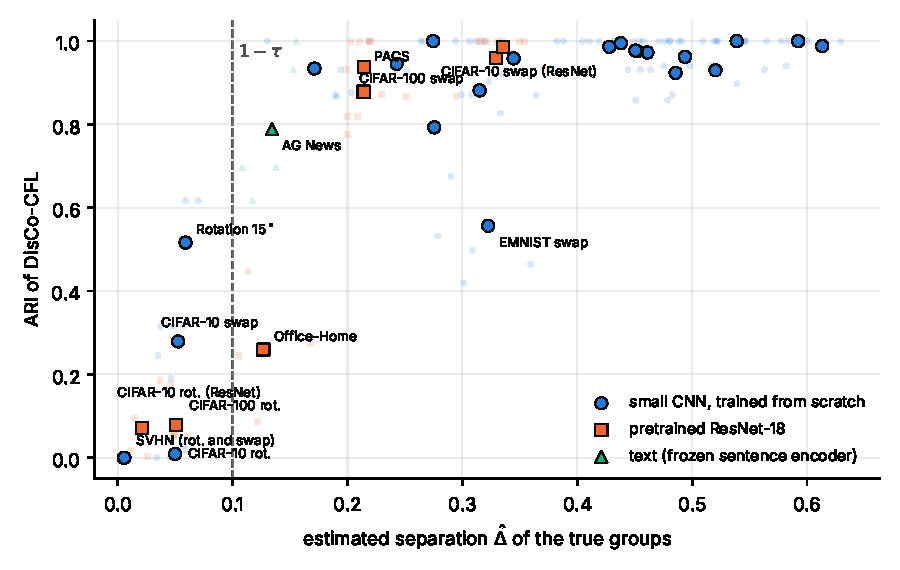
\includegraphics[width=0.85\linewidth]{../results/figures/separation.pdf}
\caption{ARI of DisCo-CFL against the estimated separation $\hat\Delta$ of the true groups, for all 31 scenarios with more than one group (large markers: means over seeds; small markers: individual runs). The dashed line is $1-\tau$, the separation that Theorem~\ref{thm:rec} requires.}\label{fig:separation}
\end{figure}


\subsection{Beyond accuracy: transparency, accountability and privacy}\label{sec:fat-exp}
\paragraph{Transparency: explanations and diagnosis (H5).}
Table~\ref{tab:fat} evaluates the class-level explanations against the ground truth. For label-swap groups the divergent classes reported by the server are \emph{exactly} the swapped classes in every pair of clusters (precision, recall and exact match $1.00$), and the diagnosis ``class-specific concept shift'' is always correct. A typical explanation reads: \emph{``cluster 0 vs.\ cluster 2: class-specific concept shift on classes [4, 5, 6, 7]''}, where group 2 swaps $4\leftrightarrow5$ and $6\leftrightarrow7$. For rotations, precision is again $1.00$: no class is reported as divergent when it is not. Recall is lower ($0.75$ for rotations, $0.78$ for \emph{Mixed + QS}). The misses are classes on which the two concepts are close at the reference model, such as nearly symmetric items under a $180^\circ$ rotation. Proposition~\ref{prop:expl} guarantees fidelity only for classes with enough pooled evidence and a separation $\Delta$, so these misses are within its scope, but they make the diagnosis ``global shift'' correct for only 43\% of the rotation pairs.

\begin{table}[!htbp]
\centering
\caption{Transparency and accountability (Fashion-MNIST, 3 seeds, default settings). Certificates: share of clients with a confident certificate, and share of correctly placed clients (no conflict with any member of their cluster) among confident and among uncertain certificates.}\label{tab:fat}
\small
\begin{tabular}{lccc}
\toprule
& Rotation & Label swap & Mixed + QS \\
\midrule
\multicolumn{4}{l}{\emph{Explanations: divergent classes between clusters}}\\
precision & 1.00 & 1.00 & 1.00 \\
recall & 0.75 & 1.00 & 0.78 \\
exact set / diagnosis correct & 0.43 & 1.00 & 0.33 \\
\midrule
\multicolumn{4}{l}{\emph{Certificates}}\\
share of confident certificates & 0.76 & 0.87 & 0.77 \\
correct among confident & 0.923 & 1.000 & 1.000 \\
correct among uncertain & 0.690 & 1.000 & 1.000 \\
\midrule
\multicolumn{4}{l}{\emph{Newcomers}}\\
known concept, correctly assigned & 0.96 & 0.96 & -- \\
novel concept, flagged as novel & 1.00 & 1.00 & -- \\
\bottomrule
\end{tabular}
\end{table}

\paragraph{Accountability: certificates, audit log, newcomers (H5).}
With the jackknife standard errors of Eq.~\eqref{eq:cert}, 76--87\% of the clients receive a confident certificate. Confident certificates are correct in all cases for label swaps and \emph{Mixed + QS}, and in 92.3\% of the cases for rotations, against 69.0\% for uncertain ones. Where every client is correctly placed, the uncertain certificates are therefore conservative, as the simulation of Section~\ref{sec:outputs} predicts; under rotations they do point to the clients whose placement is in doubt. A confident certificate is informative but not a guarantee, and we report it as an empirical rate, not as a coverage probability. Newcomers that join after clustering, using the frozen reference model, are assigned to the right cluster in 96\% of the cases, and clients with a concept never seen during clustering are reported as \emph{novel} in all cases.

\paragraph{Dependence on the reference model (pre-registered).} The reference model is trained on the clients that are then clustered. To test whether the partition depends on which clients trained it, we trained it on a random half of the clients, or on all clients except those of one concept group, and clustered all clients at that model (Table~\ref{tab:refmodel} in Appendix~\ref{app:more}; six Fashion-MNIST and MNIST scenarios, 3 seeds). Both hypotheses recorded in advance hold. With a random half, ARI changes by at most $0.05$ against the full reference model, and the label-only federation stays a single cluster; clients that did not train the model are placed slightly less well than those that did (ARI $0.91$--$1.00$ against $1.00$). A group that never contributed to the reference model is still separated: at most $1.1\%$ of the conflicting pairs that involve it are merged. In these scenarios the clustering does not hinge on which clients trained the reference model, as long as the model has learned the task; this does not extend to the datasets where it has not (Section~\ref{sec:datasets}).

\paragraph{Concept drift after clustering (pre-registered).} We tested the drift procedure proposed in Section~\ref{sec:discussion} as specified in advance: after clustering, 10\% or 20\% of the clients switch to another concept group, the server recomputes all signatures at the same reference model, and every client whose similarity to its own cluster falls below $\tau$ is flagged (Table~\ref{tab:drift} in Appendix~\ref{app:more}). Every drifted client is detected (detection rate $1.00$ in all settings), but the pre-registered criterion of at most 5\% false alarms is \emph{not} met: 31--67\% of the unchanged clients are also flagged, and 38--75\% of the drifted clients are reassigned to the cluster of their new group. The cause is that the drifted clients remain members of their old cluster and pull the bottleneck similarity of their former cluster-mates below $\tau$. In an exploratory analysis that was not pre-registered, computing each client's similarity only to the members that did not drift (in practice, members that kept a confident certificate) reduces the false-alarm rate to 1--4\% with detection unchanged. Drift detection therefore works, but needs an iterative rule that first removes the clients that changed.



\paragraph{Malicious clients.} DisCo-CFL has no defence against adversarial clients, and we measured what happens when $m\in\{1,2,4\}$ of 40 clients send manipulated signatures (Table~\ref{tab:byz} in Appendix~\ref{app:more}; no hypothesis was made). Random vectors have no split-half reliability and are flagged as low-evidence or anomalous in every run; sign-flipped signatures are isolated, alone or among themselves. Neither attack harms the clustering of the honest clients (ARI $0.95$--$0.96$, at most 0.4\% conflicting merges, as without attack). A client that copies the signature of an honest client from another group, however, is always merged into that group, without being flagged: the signature carries no information that could reveal the copy. Defending against such mimicry would need authentication of the signature or secure aggregation of the clustering step, which we leave open.



\paragraph{Privacy.}
Figure~\ref{fig:dp} shows the ARI of the clustering when the signatures are released with the Gaussian mechanism of Proposition~\ref{prop:dp} ($C_{\rm clip}=0.5$, $\delta=10^{-5}$). These results measure the utility cost of noising the clustering signal only; the warm-up and the cluster training are not private (Remark~\ref{rem:dp}). As Proposition~\ref{prop:dp}(iii) predicts, the \emph{raw} cosine collapses to ARI $\approx0$ at every noise level, with 22--40 clusters: the noise attenuates all similarities. With disattenuation the clustering degrades gradually, and more data per client buys more privacy, as the $h\propto\sigma_{\rm dp}$ term predicts. Recovery is only partial, however. With 1{,}500 samples per client, ARI is $0.75$ and $0.76$ (rotation and label swap) at $\varepsilon=10$, $0.58$ and $0.65$ at $\varepsilon=4.4$, and $0.41$ and $0.55$ at $\varepsilon=2$; with 400 samples it is at most $0.43$ at any noise level we tried. Strong privacy for the clustering signal therefore needs much larger clients than our benchmarks have.

\begin{figure}[!htbp]
\centering
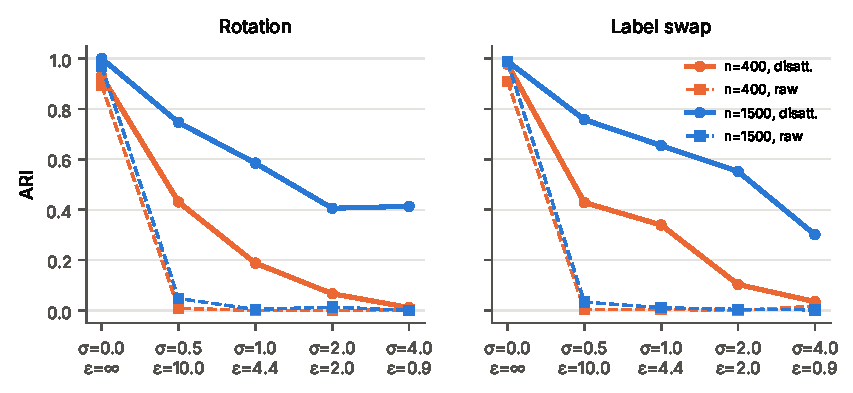
\includegraphics[width=0.85\linewidth]{../results/figures/dp.pdf}
\caption{Clustering quality under $(\varepsilon,10^{-5})$-DP signatures (3 seeds). Solid: DisCo-CFL; dashed: raw cosine. Orange: 400 samples per client; blue: 1{,}500.}\label{fig:dp}
\end{figure}

\paragraph{Class support.} The signatures reveal which classes a client holds (Section~\ref{sec:method}). Table~\ref{tab:support} (Appendix~\ref{app:more}) evaluates padding: under DP noise, every client also sends, for each class it does not hold, two independent noise vectors with the noise scale of its median class. Without padding the server knows the support exactly from the list of reported classes; even from the reliabilities alone ($R_i^c>0$) it would infer it with 77--92\% accuracy. With padding the list no longer reveals the support, but the reliabilities still do, with 63--84\% accuracy: a noise vector has a positive split-half correlation by chance in about 37\% of the cases, whereas a held class with enough data has a clearly positive one. Padding also costs clustering quality (ARI falls by up to $0.3$), because the noise classes add spurious evidence. It is therefore a weak mitigation. Hiding the support would need a mechanism that releases the support itself under DP, which we leave open.



\subsection{Calibration, sensitivity, ablation and cost}
\paragraph{Calibration and threshold (H3).}\label{sec:sens} Figure~\ref{fig:tau} varies $\tau$ on the clustering step. With disattenuation, ARI is $0.85$--$1.00$ for $\tau\in[0.85,0.95]$ in every concept-shift scenario, and the label-only scenario keeps $K=1$ up to $\tau=0.9$. With the raw cosine the useful range is narrower and higher thresholds over-split: at $\tau=0.95$ the label-only federation is split into 3 clusters and \emph{Rotation + QS} into 9.7 on average. Disattenuation therefore makes the threshold less sensitive towards high values, as H3 states. Towards low values the picture is reversed: at $\tau=0.8$ the raw cosine merges fewer groups than the disattenuated similarity (ARI $0.70$ against $0.60$ on \emph{Rotation}), because disattenuation raises all similarities, including those between groups. A calibrated scale thus shifts the useful range of $\tau$ upwards rather than widening it on both sides. The gain at the default threshold is moderate: without disattenuation (Table~\ref{tab:abl}) ARI drops by $0.04$--$0.11$ in the concept-shift scenarios and by $0.33$ in the label-only one. The sample-size study (Figure~\ref{fig:size} in Appendix~\ref{app:figs}) shows why. With clipped per-sample gradients, the raw cosine between clients of the same group is already $0.98$ on Fashion-MNIST, so there is little attenuation to correct; the disattenuated similarity is $0.99$--$1.00$. Attenuation becomes large under DP noise, where the raw cosine fails completely (Figure~\ref{fig:dp}). With very small clients (50--100 samples) both versions fail, for another reason: the groups become close at the reference model (between-group similarity $0.89$--$0.93$), i.e.\ the separation shrinks, and disattenuation does not help (ARI $0.13$--$0.63$, against $0.21$--$0.60$ for the raw cosine). Otsu's label-free threshold (Table~\ref{tab:diag}) lies at $0.76$--$0.83$ in the concept-shift scenarios. It recovers label swaps as well as $\tau=0.9$ (ARI $0.97$) but merges groups under rotations (ARI $0.58$--$0.71$). Over all scenarios (Table~\ref{tab:diag}) the comparison is two-sided. In the seven scenarios where DisCo-CFL fails (ARI below $0.5$), Otsu's threshold is better in four (e.g.\ Office-Home, $0.70$ against $0.26$; CIFAR-10 rotations with the pretrained network, $0.50$ against $0.07$), equal in the two SVHN scenarios and worse in one. In the 24 scenarios where DisCo-CFL succeeds it is lower in 19, equal in four and higher in one, and it splits single-concept federations (ARI $0$ in the label-only scenario). Its separation index $\eta$ does not distinguish successes from failures ($0.63$ for the $45^\circ$ rotation with ARI $1.00$, $0.73$ for CIFAR-10 label swaps with ARI $0.28$), so neither threshold dominates, and Otsu's rule does not replace $\tau$. The shrinkage $\lambda$ has almost no effect between $0.02$ and $1$ (Table~\ref{tab:lambda} in Appendix~\ref{app:figs}), including the values $0.02$ and $0.1$ that satisfy the condition of Corollary~\ref{cor:sc}.

\begin{figure}[!htbp]
\centering
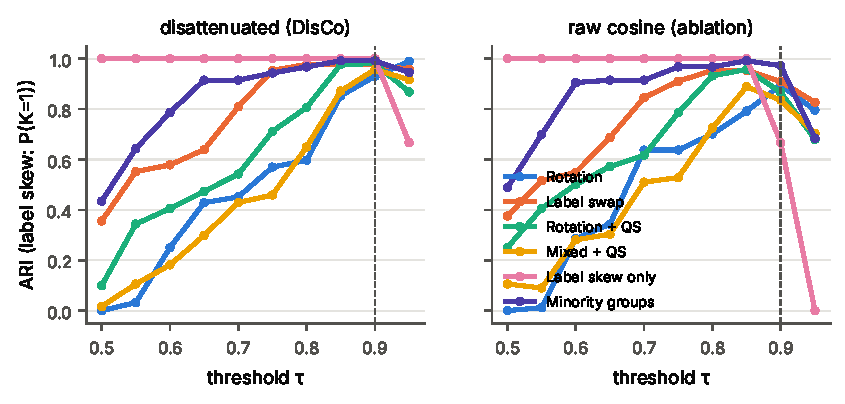
\includegraphics[width=0.85\linewidth]{../results/figures/tau_sensitivity.pdf}
\caption{Sensitivity to the threshold $\tau$ (3 seeds). The dashed line marks the default $\tau=0.9$, selected on the pilot runs (Section~\ref{sec:setup}).}\label{fig:tau}
\end{figure}

\paragraph{Edge cases.} The edge-case rules of Section~\ref{sec:method} were evaluated in three federations (Table~\ref{tab:edge} in Appendix~\ref{app:more}): the default minimum class size $m=4$ is best or close to best, the reliability floor $r_{\min}$ has no measurable effect, and extreme label skew ($\alpha=0.1$) or small clients lower ARI to about $0.7$.

\paragraph{Theory in practice.} On synthetic signatures with known ground truth the disattenuated similarity is nearly unbiased, whereas the raw cosine is biased by up to $-0.37$, and the guarantees of Theorem~\ref{thm:rec} are reached once $h\ge64$ (Figure~\ref{fig:theory} in Appendix~\ref{app:more}).

\paragraph{Ablation (H3, H4).}
Table~\ref{tab:abl} removes one component at a time. Without class conditioning (one signature per client over all its data), clients are grouped by their label mix, the failure mode reported in the survey~\citep{benali2026survey}: 18--33 clusters and a concept accuracy 19 points lower. The mean linkage averages class-specific shifts away and merges conflicting clients (11.3\% on average, ARI $0.48$ under rotations), which supports H4: the minimum over classes matters. Linkage-ordered merging over-splits label swaps and \emph{Mixed + QS}. Without disattenuation or without clipping the federation is split more often, most visibly in the label-only scenario. Without the attachment stage, a noisy client stays alone in the label-only scenario in one of the three seeds. The table uses seeds 0--2 for all rows, so the DisCo-CFL row differs slightly from the five-seed means of Table~\ref{tab:main}. The ablation supports class conditioning and the bottleneck linkage clearly; evidence-ordered merging and clipping matter only in some scenarios (linkage-ordered merging is slightly better on \emph{Rotation} and \emph{Rotation + QS}), and these two choices rest mainly on the pilot runs.

\begin{table}[!htbp]
\centering
\caption{Ablation (Fashion-MNIST, 3 seeds): ARI / number of clusters $K$ per scenario, mean conflict-merge rate (\%) and mean concept accuracy (\%) over the five scenarios.}\label{tab:abl}
\scriptsize
\setlength{\tabcolsep}{3pt}
\begin{tabular}{lccccccc}
\toprule
Variant & Rotation & Label swap & Rot.\,+\,QS & Mixed\,+\,QS & Label only & Conflict\% & Concept \\
\midrule
DisCo-CFL (full) & 0.93 / 4.3 & 0.98 / 4.0 & 0.98 / 4.3 & 0.96 / 4.0 & 1.00 / 1.0 & 0.2 & 76.9 \\
without disattenuation (raw cosine) & 0.89 / 5.0 & 0.91 / 4.7 & 0.87 / 5.3 & 0.86 / 5.0 & 0.67 / 1.3 & 0.4 & 76.0 \\
without class conditioning & 0.05 / 31.7 & 0.04 / 32.7 & 0.03 / 33.0 & 0.02 / 29.0 & 0.00 / 17.7 & 0.8 & 57.9 \\
mean instead of bottleneck linkage & 0.48 / 3.0 & 0.70 / 4.0 & 0.79 / 4.0 & 0.58 / 4.0 & 1.00 / 1.0 & 11.3 & 73.6 \\
linkage-ordered merging & 0.95 / 4.7 & 0.85 / 5.3 & 0.97 / 4.3 & 0.77 / 6.3 & 0.67 / 1.3 & 0.0 & 75.7 \\
without per-sample clipping & 0.93 / 4.3 & 1.00 / 4.0 & 0.93 / 5.0 & 0.93 / 4.3 & 0.33 / 1.7 & 0.2 & 76.6 \\
without attachment stage & 0.91 / 5.0 & 0.98 / 4.0 & 0.97 / 4.7 & 0.96 / 4.0 & 0.67 / 1.3 & 0.1 & 76.7 \\
\bottomrule
\end{tabular}
\end{table}

\paragraph{Cost and scalability.}\label{sec:cost}
Table~\ref{tab:cost} reports wall-clock time per run and the floats each client uploads for clustering. Each DisCo-CFL client uploads its signature \emph{once}, $2p|S_i|\le2pC\approx2.0\times10^4$ floats with $p=1024$ ($1.7$--$2.0\times10^4$ on average in Table~\ref{tab:cost}), independent of the model dimension $d$ (46{,}730 for the small CNN, 8.4M for the ResNet-18 block). FL+HC and StoCFL upload $d$-dimensional updates or gradients for clustering, IFCA downloads $K$ models per client in every round, and FedCCFA exchanges classifiers and class anchors in every round. A DisCo-CFL run takes about as long as a FedAvg run (the times come from shared machines, so differences below about 20\% are noise; FedAvg-FT appears faster than FedAvg on the realistic benchmarks for this reason); StoCFL takes about twice as long because it trains two models per round. Computing the signature takes about 0.09\,s per client on one CPU core, and server-side clustering 0.09\,s for 40 clients and 6\,s for 320 clients. In the clustering-only scalability study, which uses 200 samples per client, ARI is $0.59$--$0.82$ for 40 to 320 clients. With 200 clients in the full pipeline (Table~\ref{tab:sweeps}) ARI is $0.88$ and accuracy is within $0.7$ points of the Oracle. The scalability study uses one seed per size and its ARI is not monotone in the number of clients, so it measures time rather than recovery.

\begin{table}[!htbp]
\centering
\caption{Cost per run: mean wall-clock time (minutes; one CPU core for the small CNN, one GPU for the realistic benchmarks) and floats uploaded per client for the clustering signal.}\label{tab:cost}
{\scriptsize
\begin{tabular}{l c c c}
\toprule
Method & Time, small-CNN main (min) & Time, realistic (min) & Upload floats / client \\
\midrule
DisCo & 6.9 & 1.4 & 1.4e4 \\
DisCo-noAttach & 6.9 & 1.5 & 1.5e4 \\
FedAvg & 7.1 & 1.5 & 0 \\
Local & 6.9 & 1.4 & 0 \\
FedAvg-FT & 7.6 & 1.2 & 0 \\
IFCA & 11.0 & 2.8 & 0 \\
FeSEM & 7.7 & 1.6 & 0 \\
MTCFL & 6.1 & 1.3 & 0 \\
FL+HC & 7.6 & 1.6 & 1.7e6 \\
PACFL & 7.5 & 1.5 & 2.3e3 \\
StoCFL & 13.9 & 3.2 & 1.8e6 \\
StoCFL-W & 12.5 & 4.4 & 1.9e5 \\
FedCCFA & 5.2 & 3.7 & 3.8e5 \\
FedDAG-C & 7.9 & 1.5 & 4.8e4 \\
Oracle & 7.2 & 1.4 & 0 \\
DisCo-linkorder & 6.3 & -- & 1.2e4 \\
DisCo-mean & 6.0 & -- & 1.2e4 \\
DisCo-noClass & 6.0 & -- & 2.0e3 \\
DisCo-noClip & 5.9 & -- & 1.2e4 \\
DisCo-noDisatt & 6.0 & -- & 1.2e4 \\
\bottomrule
\end{tabular}
}

\end{table}


\subsection{Pretrained network: natural domain shift, CIFAR-100 and FEMNIST}\label{sec:real}
The benchmarks above use small CNNs trained from scratch on images with synthetic concept groups. Here the clients of PACS and Office-Home differ by a natural domain shift, CIFAR-100 has synthetic groups on a harder dataset, and all three use the pretrained ResNet-18 (Section~\ref{sec:setup}); FEMNIST, at the end of the section, has natural heterogeneity without ground-truth groups.

\begin{table}[!htbp]
\centering
\caption{PACS, PACS with quantity skew, Office-Home and CIFAR-100 (40 clients, 5 seeds; DisCo-T30: 3 seeds). Columns as in Table~\ref{tab:main}; IFCA, FeSEM, FL+HC, PACFL and FedDAG-C receive the true $K=4$. The last block repeats FEMNIST (Table~\ref{tab:real_femnist}); there ARI is computed against a single group and is not meaningful.}\label{tab:real}
{\scriptsize
\begin{tabular}{l r c c c c c c}
\toprule
Method & n & Acc (\%) & Concept (\%) & Worst-grp (\%) & ARI & K & Conflict (\%) \\
\midrule
\multicolumn{8}{l}{\textit{PACS}} \\
DisCo & 5 & 93.3 $\pm$ 1.1 & 85.4 $\pm$ 1.7 & 90.0 $\pm$ 2.2 & 0.94 $\pm$ 0.11 & 4.0 & 1.7 \\
DisCo-noAttach & 5 & 93.3 $\pm$ 1.1 & 85.3 $\pm$ 1.6 & 90.0 $\pm$ 2.3 & 0.93 $\pm$ 0.10 & 4.2 & 1.7 \\
DisCo-T30 & 3 & 92.7 $\pm$ 3.1 & 84.6 $\pm$ 1.6 & 88.0 $\pm$ 7.6 & 0.88 $\pm$ 0.26 & 5.0 & 1.7 \\
FedAvg & 5 & 90.9 $\pm$ 1.1 & 81.3 $\pm$ 1.6 & 87.0 $\pm$ 2.3 & 0.00 $\pm$ 0.00 & 1.0 & 100.0 \\
Local & 5 & 89.7 $\pm$ 1.2 & 55.5 $\pm$ 3.1 & 84.5 $\pm$ 3.2 & 0.00 $\pm$ 0.00 & 40.0 & 0.0 \\
FedAvg-FT & 5 & 81.1 $\pm$ 3.5 & 72.2 $\pm$ 2.1 & 70.4 $\pm$ 4.7 & 0.00 $\pm$ 0.00 & 40.0 & 0.0 \\
IFCA & 5 & 91.0 $\pm$ 1.6 & 76.0 $\pm$ 3.4 & 86.8 $\pm$ 3.4 & 0.17 $\pm$ 0.12 & 4.0 & 22.5 \\
FeSEM & 5 & 91.3 $\pm$ 0.9 & 79.5 $\pm$ 1.7 & 87.7 $\pm$ 1.8 & 0.01 $\pm$ 0.04 & 4.0 & 61.8 \\
MTCFL & 5 & 91.1 $\pm$ 2.9 & 72.6 $\pm$ 2.2 & 86.4 $\pm$ 7.3 & 0.05 $\pm$ 0.03 & 25.2 & 1.1 \\
FL+HC & 5 & 91.4 $\pm$ 1.4 & 79.0 $\pm$ 1.6 & 87.2 $\pm$ 2.4 & 0.09 $\pm$ 0.13 & 4.0 & 44.2 \\
PACFL & 5 & 91.5 $\pm$ 0.8 & 81.3 $\pm$ 2.1 & 87.6 $\pm$ 3.2 & 0.30 $\pm$ 0.06 & 4.0 & 32.6 \\
StoCFL & 5 & 90.9 $\pm$ 1.1 & 72.1 $\pm$ 1.8 & 86.7 $\pm$ 3.2 & 0.07 $\pm$ 0.03 & 11.0 & 10.8 \\
StoCFL-W & 5 & 91.4 $\pm$ 1.4 & 75.8 $\pm$ 3.1 & 88.0 $\pm$ 3.1 & 0.09 $\pm$ 0.07 & 12.6 & 7.6 \\
FedCCFA & 5 & 90.0 $\pm$ 1.2 & 78.0 $\pm$ 1.0 & 85.3 $\pm$ 2.3 & 0.00 $\pm$ 0.00 & 1.0 & 100.0 \\
FedDAG-C & 5 & 90.9 $\pm$ 1.3 & 76.4 $\pm$ 3.8 & 87.2 $\pm$ 3.1 & 0.10 $\pm$ 0.16 & 4.0 & 44.2 \\
Oracle & 5 & 93.4 $\pm$ 1.1 & 85.8 $\pm$ 1.3 & 90.1 $\pm$ 2.3 & 1.00 $\pm$ 0.00 & 4.0 & 0.0 \\
\addlinespace
\multicolumn{8}{l}{\textit{PACS + QS}} \\
DisCo & 5 & 92.6 $\pm$ 0.4 & 85.6 $\pm$ 2.0 & 89.0 $\pm$ 1.0 & 0.88 $\pm$ 0.11 & 4.0 & 3.3 \\
DisCo-noAttach & 5 & 92.6 $\pm$ 0.4 & 85.6 $\pm$ 1.9 & 89.0 $\pm$ 0.9 & 0.88 $\pm$ 0.11 & 4.0 & 3.3 \\
FedAvg & 5 & 90.4 $\pm$ 0.5 & 80.1 $\pm$ 2.7 & 86.4 $\pm$ 1.5 & 0.00 $\pm$ 0.00 & 1.0 & 100.0 \\
Local & 5 & 87.1 $\pm$ 1.2 & 51.0 $\pm$ 2.5 & 81.8 $\pm$ 2.6 & 0.00 $\pm$ 0.00 & 40.0 & 0.0 \\
FedAvg-FT & 5 & 85.3 $\pm$ 1.1 & 74.6 $\pm$ 2.9 & 75.4 $\pm$ 5.3 & 0.00 $\pm$ 0.00 & 40.0 & 0.0 \\
IFCA & 5 & 90.0 $\pm$ 0.7 & 76.7 $\pm$ 3.8 & 85.5 $\pm$ 1.8 & 0.27 $\pm$ 0.23 & 4.0 & 19.5 \\
FeSEM & 5 & 89.7 $\pm$ 0.6 & 77.1 $\pm$ 3.4 & 84.6 $\pm$ 2.4 & 0.06 $\pm$ 0.05 & 4.0 & 48.2 \\
MTCFL & 5 & 90.3 $\pm$ 1.2 & 71.8 $\pm$ 2.1 & 85.3 $\pm$ 2.9 & 0.06 $\pm$ 0.01 & 25.6 & 0.9 \\
FL+HC & 5 & 89.5 $\pm$ 0.8 & 76.9 $\pm$ 3.4 & 84.4 $\pm$ 4.0 & 0.03 $\pm$ 0.03 & 4.0 & 39.0 \\
PACFL & 5 & 90.6 $\pm$ 1.0 & 79.2 $\pm$ 4.1 & 86.0 $\pm$ 3.6 & 0.45 $\pm$ 0.13 & 4.0 & 18.7 \\
StoCFL & 5 & 88.9 $\pm$ 1.4 & 68.6 $\pm$ 4.1 & 85.4 $\pm$ 1.6 & 0.05 $\pm$ 0.03 & 10.6 & 10.6 \\
StoCFL-W & 5 & 89.9 $\pm$ 1.1 & 74.5 $\pm$ 1.2 & 84.4 $\pm$ 3.9 & 0.07 $\pm$ 0.05 & 14.2 & 7.7 \\
FedCCFA & 5 & 89.9 $\pm$ 0.3 & 78.2 $\pm$ 2.6 & 85.4 $\pm$ 2.3 & 0.00 $\pm$ 0.00 & 1.2 & 99.0 \\
FedDAG-C & 5 & 89.1 $\pm$ 0.6 & 72.2 $\pm$ 3.5 & 84.7 $\pm$ 2.5 & 0.06 $\pm$ 0.07 & 4.0 & 36.9 \\
Oracle & 5 & 92.7 $\pm$ 0.5 & 85.8 $\pm$ 1.8 & 89.1 $\pm$ 0.8 & 1.00 $\pm$ 0.00 & 4.0 & 0.0 \\
\addlinespace
\multicolumn{8}{l}{\textit{Office-Home}} \\
DisCo & 5 & 69.5 $\pm$ 1.2 & 57.7 $\pm$ 2.9 & 55.4 $\pm$ 4.4 & 0.26 $\pm$ 0.16 & 3.6 & 33.6 \\
DisCo-noAttach & 5 & 69.5 $\pm$ 1.2 & 57.3 $\pm$ 3.1 & 55.5 $\pm$ 4.4 & 0.26 $\pm$ 0.16 & 4.0 & 33.1 \\
DisCo-T30 & 3 & 70.0 $\pm$ 2.6 & 59.5 $\pm$ 5.3 & 55.3 $\pm$ 4.8 & 0.41 $\pm$ 0.41 & 4.3 & 19.1 \\
FedAvg & 5 & 69.4 $\pm$ 1.5 & 58.4 $\pm$ 1.4 & 57.5 $\pm$ 3.4 & 0.00 $\pm$ 0.00 & 1.0 & 100.0 \\
Local & 5 & 61.6 $\pm$ 0.6 & 23.8 $\pm$ 1.0 & 49.1 $\pm$ 1.2 & 0.00 $\pm$ 0.00 & 40.0 & 0.0 \\
FedAvg-FT & 5 & 65.9 $\pm$ 1.7 & 55.4 $\pm$ 1.2 & 54.4 $\pm$ 2.8 & 0.00 $\pm$ 0.00 & 40.0 & 0.0 \\
IFCA & 5 & 67.6 $\pm$ 1.0 & 51.6 $\pm$ 2.0 & 55.5 $\pm$ 2.3 & 0.04 $\pm$ 0.08 & 4.0 & 29.8 \\
FeSEM & 5 & 68.7 $\pm$ 1.4 & 55.1 $\pm$ 2.0 & 56.3 $\pm$ 2.4 & 0.09 $\pm$ 0.09 & 4.0 & 34.6 \\
MTCFL & 5 & 67.6 $\pm$ 0.6 & 43.6 $\pm$ 1.2 & 55.1 $\pm$ 0.8 & 0.11 $\pm$ 0.02 & 24.2 & 0.3 \\
FL+HC & 5 & 69.8 $\pm$ 2.0 & 58.8 $\pm$ 2.7 & 54.9 $\pm$ 4.2 & 0.52 $\pm$ 0.30 & 4.0 & 22.6 \\
PACFL & 5 & 69.4 $\pm$ 2.2 & 56.1 $\pm$ 2.4 & 58.9 $\pm$ 3.7 & 0.30 $\pm$ 0.09 & 4.0 & 28.0 \\
StoCFL & 5 & 62.8 $\pm$ 0.8 & 27.4 $\pm$ 2.8 & 49.9 $\pm$ 1.4 & 0.01 $\pm$ 0.01 & 35.6 & 0.9 \\
StoCFL-W & 5 & 66.6 $\pm$ 0.6 & 34.3 $\pm$ 1.0 & 54.9 $\pm$ 1.9 & 0.00 $\pm$ 0.01 & 39.2 & 0.0 \\
FedCCFA & 5 & 67.7 $\pm$ 1.2 & 56.6 $\pm$ 1.3 & 54.5 $\pm$ 2.2 & 0.00 $\pm$ 0.00 & 1.0 & 100.0 \\
FedDAG-C & 5 & 68.1 $\pm$ 1.3 & 53.5 $\pm$ 1.3 & 53.3 $\pm$ 3.8 & 0.17 $\pm$ 0.17 & 4.0 & 35.8 \\
Oracle & 5 & 70.4 $\pm$ 1.1 & 61.5 $\pm$ 1.8 & 54.9 $\pm$ 2.9 & 1.00 $\pm$ 0.00 & 4.0 & 0.0 \\
\addlinespace
\bottomrule
\end{tabular}
}


\end{table}

\begin{table}[!htbp]
\centering
\caption*{Table~\ref{tab:real} (continued).}
{\scriptsize
\begin{tabular}{l r c c c c c c}
\toprule
Method & n & Acc (\%) & Concept (\%) & Worst-grp (\%) & ARI & K & Conflict (\%) \\
\midrule
\multicolumn{8}{l}{\textit{CIFAR-100 label swaps}} \\
DisCo & 5 & 57.8 $\pm$ 0.9 & 47.4 $\pm$ 0.8 & 56.2 $\pm$ 0.4 & 0.96 $\pm$ 0.07 & 4.0 & 0.7 \\
DisCo-noAttach & 5 & 57.6 $\pm$ 0.9 & 47.0 $\pm$ 1.2 & 56.0 $\pm$ 0.6 & 0.94 $\pm$ 0.09 & 4.6 & 0.7 \\
FedAvg & 5 & 53.9 $\pm$ 0.8 & 44.5 $\pm$ 0.8 & 51.0 $\pm$ 0.6 & 0.00 $\pm$ 0.00 & 1.0 & 100.0 \\
Local & 5 & 42.0 $\pm$ 0.6 & 17.0 $\pm$ 0.2 & 40.8 $\pm$ 0.7 & 0.00 $\pm$ 0.00 & 40.0 & 0.0 \\
FedAvg-FT & 5 & 51.8 $\pm$ 0.7 & 41.1 $\pm$ 0.4 & 50.1 $\pm$ 0.9 & 0.00 $\pm$ 0.00 & 40.0 & 0.0 \\
IFCA & 5 & 49.8 $\pm$ 0.6 & 38.0 $\pm$ 1.1 & 47.5 $\pm$ 1.2 & 0.03 $\pm$ 0.07 & 4.0 & 28.9 \\
FeSEM & 5 & 52.7 $\pm$ 1.4 & 40.9 $\pm$ 1.3 & 49.9 $\pm$ 1.2 & 0.11 $\pm$ 0.11 & 4.0 & 31.8 \\
MTCFL & 5 & 51.2 $\pm$ 0.9 & 31.4 $\pm$ 1.2 & 49.6 $\pm$ 1.5 & 0.09 $\pm$ 0.03 & 25.4 & 0.4 \\
FL+HC & 5 & 55.8 $\pm$ 1.5 & 44.9 $\pm$ 1.5 & 53.1 $\pm$ 2.6 & 0.48 $\pm$ 0.20 & 4.0 & 21.1 \\
PACFL & 5 & 51.6 $\pm$ 1.0 & 40.3 $\pm$ 1.4 & 49.3 $\pm$ 1.7 & $-$0.01 $\pm$ 0.01 & 4.0 & 62.4 \\
StoCFL & 5 & 53.7 $\pm$ 0.6 & 44.0 $\pm$ 1.4 & 50.6 $\pm$ 0.9 & $-$0.00 $\pm$ 0.00 & 1.8 & 95.8 \\
StoCFL-W & 5 & 48.9 $\pm$ 0.8 & 24.4 $\pm$ 0.5 & 47.1 $\pm$ 1.2 & 0.00 $\pm$ 0.00 & 40.0 & 0.0 \\
FedCCFA & 5 & 54.8 $\pm$ 0.8 & 43.3 $\pm$ 0.8 & 52.5 $\pm$ 1.2 & $-$0.00 $\pm$ 0.01 & 11.4 & 54.3 \\
FedDAG-C & 5 & 51.7 $\pm$ 1.3 & 39.9 $\pm$ 0.8 & 48.0 $\pm$ 1.1 & 0.11 $\pm$ 0.04 & 4.0 & 31.4 \\
Oracle & 5 & 58.1 $\pm$ 0.7 & 47.8 $\pm$ 0.9 & 56.4 $\pm$ 0.7 & 1.00 $\pm$ 0.00 & 4.0 & 0.0 \\
\addlinespace
\multicolumn{8}{l}{\textit{CIFAR-100 rotations}} \\
DisCo & 5 & 51.2 $\pm$ 1.0 & 40.3 $\pm$ 1.2 & 48.5 $\pm$ 1.8 & 0.08 $\pm$ 0.07 & 2.6 & 59.7 \\
DisCo-noAttach & 5 & 51.2 $\pm$ 0.9 & 40.1 $\pm$ 1.1 & 48.4 $\pm$ 1.5 & 0.08 $\pm$ 0.07 & 3.0 & 58.9 \\
DisCo-T30 & 3 & 52.2 $\pm$ 0.9 & 41.4 $\pm$ 2.5 & 49.3 $\pm$ 2.2 & 0.01 $\pm$ 0.01 & 2.3 & 71.0 \\
FedAvg & 5 & 52.7 $\pm$ 0.5 & 42.1 $\pm$ 0.7 & 50.1 $\pm$ 1.0 & 0.00 $\pm$ 0.00 & 1.0 & 100.0 \\
Local & 5 & 37.2 $\pm$ 0.8 & 14.5 $\pm$ 0.1 & 33.8 $\pm$ 0.8 & 0.00 $\pm$ 0.00 & 40.0 & 0.0 \\
FedAvg-FT & 5 & 46.0 $\pm$ 0.9 & 37.0 $\pm$ 0.5 & 42.4 $\pm$ 0.7 & 0.00 $\pm$ 0.00 & 40.0 & 0.0 \\
IFCA & 5 & 47.8 $\pm$ 0.9 & 35.3 $\pm$ 1.1 & 44.2 $\pm$ 1.5 & 0.02 $\pm$ 0.09 & 4.0 & 29.9 \\
FeSEM & 5 & 49.0 $\pm$ 1.0 & 37.1 $\pm$ 1.2 & 45.8 $\pm$ 2.1 & 0.01 $\pm$ 0.06 & 4.0 & 30.4 \\
MTCFL & 5 & 45.1 $\pm$ 0.3 & 26.1 $\pm$ 0.8 & 41.8 $\pm$ 0.7 & 0.04 $\pm$ 0.03 & 25.6 & 1.2 \\
FL+HC & 5 & 50.4 $\pm$ 0.7 & 38.6 $\pm$ 1.2 & 47.4 $\pm$ 1.3 & 0.06 $\pm$ 0.08 & 4.0 & 44.9 \\
PACFL & 5 & 51.6 $\pm$ 0.9 & 40.3 $\pm$ 0.9 & 48.3 $\pm$ 2.4 & 0.47 $\pm$ 0.05 & 4.0 & 27.7 \\
StoCFL & 5 & 52.2 $\pm$ 0.5 & 41.2 $\pm$ 0.6 & 49.1 $\pm$ 1.6 & 0.00 $\pm$ 0.00 & 2.2 & 94.1 \\
StoCFL-W & 5 & 43.5 $\pm$ 0.5 & 20.9 $\pm$ 0.4 & 40.0 $\pm$ 0.4 & 0.00 $\pm$ 0.00 & 40.0 & 0.0 \\
FedCCFA & 5 & 49.7 $\pm$ 0.6 & 39.8 $\pm$ 0.7 & 46.1 $\pm$ 1.3 & $-$0.00 $\pm$ 0.01 & 9.8 & 60.5 \\
FedDAG-C & 5 & 49.6 $\pm$ 1.4 & 37.1 $\pm$ 1.8 & 46.4 $\pm$ 2.1 & 0.02 $\pm$ 0.01 & 4.0 & 48.9 \\
Oracle & 5 & 51.7 $\pm$ 0.4 & 41.2 $\pm$ 0.5 & 48.1 $\pm$ 0.6 & 1.00 $\pm$ 0.00 & 4.0 & 0.0 \\
\addlinespace
\multicolumn{8}{l}{\textit{FEMNIST}} \\
DisCo & 5 & 62.8 $\pm$ 0.9 & 58.6 $\pm$ 3.1 & 62.8 $\pm$ 0.9 & 0.80 $\pm$ 0.56 & 1.2 & 0.0 \\
DisCo-noAttach & 5 & 62.8 $\pm$ 0.9 & 58.6 $\pm$ 3.1 & 62.8 $\pm$ 0.9 & 0.80 $\pm$ 0.56 & 1.2 & 0.0 \\
FedAvg & 5 & 62.8 $\pm$ 0.9 & 58.7 $\pm$ 3.2 & 62.8 $\pm$ 0.9 & 1.00 $\pm$ 0.00 & 1.0 & 0.0 \\
Local & 5 & 63.6 $\pm$ 1.1 & 24.7 $\pm$ 2.1 & 63.6 $\pm$ 1.1 & 0.00 $\pm$ 0.00 & 100.0 & 0.0 \\
FedAvg-FT & 5 & 55.3 $\pm$ 0.9 & 43.5 $\pm$ 2.8 & 55.3 $\pm$ 0.9 & 0.00 $\pm$ 0.00 & 100.0 & 0.0 \\
IFCA & 5 & 65.2 $\pm$ 2.3 & 55.3 $\pm$ 5.0 & 65.2 $\pm$ 2.3 & 0.20 $\pm$ 0.56 & 2.0 & 0.0 \\
FeSEM & 5 & 64.6 $\pm$ 1.1 & 51.3 $\pm$ 4.7 & 64.6 $\pm$ 1.1 & 0.00 $\pm$ 0.00 & 3.6 & 0.0 \\
MTCFL & 5 & 63.0 $\pm$ 1.3 & 30.7 $\pm$ 2.7 & 63.0 $\pm$ 1.3 & 0.00 $\pm$ 0.00 & 65.0 & 0.0 \\
FL+HC & 5 & 63.9 $\pm$ 0.6 & 50.6 $\pm$ 4.2 & 63.9 $\pm$ 0.6 & 0.00 $\pm$ 0.00 & 4.0 & 0.0 \\
StoCFL & 5 & 62.7 $\pm$ 0.9 & 56.6 $\pm$ 4.6 & 62.7 $\pm$ 0.9 & 0.60 $\pm$ 0.68 & 1.4 & 0.0 \\
StoCFL-W & 5 & 64.5 $\pm$ 0.6 & 51.9 $\pm$ 3.6 & 64.5 $\pm$ 0.6 & 0.00 $\pm$ 0.00 & 6.0 & 0.0 \\
FedCCFA & 5 & 62.7 $\pm$ 1.3 & 53.5 $\pm$ 2.5 & 62.7 $\pm$ 1.3 & 0.40 $\pm$ 0.68 & 2.0 & 0.0 \\
FedDAG-C & 5 & 64.5 $\pm$ 0.6 & 50.7 $\pm$ 3.6 & 64.5 $\pm$ 0.6 & 0.00 $\pm$ 0.00 & 4.0 & 0.0 \\
\bottomrule
\end{tabular}
}


\end{table}

\paragraph{Where DisCo-CFL works.} On PACS (Table~\ref{tab:real}) DisCo-CFL recovers the domains in most runs (ARI $0.94\pm0.11$, 1.7\% of the conflicting pairs merged) and matches the Oracle in accuracy (93.3\% against 93.4\%), concept accuracy and worst-group accuracy. The best baselines, PACFL and FL+HC, reach 91.4--91.5\% with ARI at most $0.30$, and FedAvg 90.9\%. With quantity skew (PACS + QS) the picture is the same: 92.6\% against 92.7\% for the Oracle and 90.6\% for the best baseline (PACFL), ARI $0.88$. With label-swap groups on CIFAR-100, DisCo-CFL finds the groups without being told $K$ (ARI $0.96$, 0.7\% conflicting merges) and reaches 57.8\% (Oracle 58.1\%), against 55.8\% for FL+HC, the best baseline, and 53.9\% for FedAvg. The estimated separation is $\hat\Delta=0.21$ on PACS and $0.33$ on CIFAR-100 label swaps (Table~\ref{tab:diag}).

\paragraph{Where it does not.} On Office-Home and on rotated CIFAR-100, DisCo-CFL does not separate the groups: ARI $0.26$ and $0.08$, with 34\% and 60\% of the conflicting pairs merged. The cost in accuracy is small because there is little to gain: the Oracle improves on FedAvg by $1.0$ point on Office-Home and is $1.0$ point \emph{below} FedAvg on rotated CIFAR-100, where the pretrained features make one model sufficient. DisCo-CFL is at the level of FedAvg on Office-Home (69.5\% against 69.4\%) and $1.5$ points below it on rotated CIFAR-100 (51.2\% against 52.7\%), because it trains a few clusters with less data each. The baselines that receive the true $K$ separate these groups better but still only partly: the best ARI is $0.52$ (FL+HC) on Office-Home and $0.47$ (PACFL) on rotated CIFAR-100, and neither is more than $0.4$ points more accurate than FedAvg. The diagnostics differ between the two failures. Rotated CIFAR-100 has $\hat\Delta=0.05$, below $1-\tau$: the reference model does not separate rotations of natural images, much as on CIFAR-10. Office-Home has $\hat\Delta=0.13$, just above $1-\tau=0.1$, so the margin $\gamma$ of Theorem~\ref{thm:rec} is about $0.03$ and the finite-sample condition is not met; here Otsu's label-free threshold ($0.94$) recovers more of the structure than the default (ARI $0.70$ against $0.26$, Table~\ref{tab:diag}). Table~\ref{tab:real_variants} in Appendix~\ref{app:more} reports two attempted remedies (3 seeds). A signature from the gradient of the whole layer-4 block raises ARI to $0.75$ on Office-Home and $0.32$ on rotated CIFAR-100, and a 30-round warm-up to $0.41$ and $0.01$; only the full-layer signature improves the clustering, and neither changes accuracy by more than $1.4$ points, consistent with the small gain available.



\paragraph{Ablation on CIFAR-100 label swaps.} Table~\ref{tab:real_ablation} in Appendix~\ref{app:more} removes one component at a time (3 seeds). Here every main component matters. Without class conditioning, clients are grouped by their label mix: every client is alone ($K=40$), and accuracy falls by 10 points. Without disattenuation, the 100-class signatures are noisy and the federation is split into 16 clusters (ARI $0.26$; accuracy $-7.2$ points), which supports H3 more clearly than the Fashion-MNIST ablation. With the mean instead of the bottleneck, the swaps, which touch 20 of the 100 classes, are averaged away and all groups are merged ($K=1.3$, 96\% conflicting merges; $-3.7$ points), which supports H4. Linkage-ordered merging over-splits ($K=7.7$, ARI $0.68$); clipping and attachment make little difference.



\paragraph{Statistical comparison.} Over the five realistic benchmarks, the hierarchical bootstrap gives DisCo-CFL a positive mean difference in accuracy against every baseline (Table~\ref{tab:hier}, part b), with intervals that exclude zero except against FedAvg ($+1.4$, $[-0.3,+3.1]$). With five scenarios the smallest possible Wilcoxon $p$-value is $0.031$, so these tests have little power, and the per-benchmark results above are the more informative summary: clear gains on PACS and CIFAR-100 label swaps, none on Office-Home, and a small loss on rotated CIFAR-100.

\paragraph{FEMNIST: natural writers without ground-truth groups.} FEMNIST has no true number of groups, so the $K=4$ given to IFCA, FeSEM, FL+HC and FedDAG-C has no justification. DisCo-CFL forms one cluster in four of the five seeds and two in the fifth, and its accuracy equals that of FedAvg (62.8\%; Table~\ref{tab:real_femnist}). Methods that split the writers into a few clusters are 1.7--2.4 points more accurate on local test data (IFCA 65.2\%, FeSEM 64.6\%, FedDAG-C and StoCFL-W 64.5\%), but generalise less to other writers (pooled accuracy 50.7--55.3\% against 58.6\% for DisCo-CFL and 58.7\% for FedAvg). With a reference model of 10 rounds, the writers' class-conditional gradients are not separated enough for DisCo-CFL to split them, so on natural writer heterogeneity it reduces to FedAvg.

\begin{table}[!htbp]
\centering
\caption{FEMNIST, 100 writers, 5 seeds. Pooled: accuracy on the pooled test sets of 20 writers. IFCA, FeSEM, FL+HC and FedDAG-C receive $K=4$.}\label{tab:real_femnist}
\scriptsize
\setlength{\tabcolsep}{3.5pt}
\begin{tabular}{lcccc}
\toprule
Method & Acc & Acc@10\% & Pooled & $K$ \\
\midrule
\multicolumn{5}{l}{\textit{FEMNIST (100 writers)}}\\
FedAvg & 62.7 & 47.5 & \textbf{57.7} & 1.0 \\
Local & 63.8 & 48.3 & 22.7 & 100.0 \\
FedAvg-FT & 54.5 & 32.2 & 42.3 & 100.0 \\
IFCA & \textbf{66.8} & \textbf{52.4} & 56.6 & 3.0 \\
FeSEM & 63.9 & 51.6 & 47.4 & 4.0 \\
MTCFL & 61.9 & 47.2 & 28.5 & 65.0 \\
FL+HC & 63.2 & 48.3 & 48.4 & 4.0 \\
\bottomrule
\end{tabular}

\end{table}

\subsection{Additional pre-registered benchmarks}\label{sec:extra}
To test the scope stated above on data not used so far, we ran seven further scenarios whose choice and hypotheses were recorded in the repository before any of them was run (file \texttt{PREREGISTRATION\_R1\_EXTRA.md}): CIFAR-10 with the pretrained ResNet-18 of Section~\ref{sec:real}, where the small-CNN failure was attributed to an uninformative reference model; a text benchmark, AG News with a frozen sentence encoder~\citep{reimers2019sbert} and a two-layer classifier head; and KMNIST and EMNIST (47 classes) with the small CNN. Rotation and label-swap groups are built as before, all hyperparameters are unchanged, and every method was run with five seeds. The only choice made for the new data is the learning rate of the text model, which, as for PACS, was selected with FedAvg on a single-concept federation after standardising the embeddings; this amendment was recorded before any run of the compared methods. Table~\ref{tab:extra} reports all results.

\begin{table}[!htbp]
\centering
\caption{Additional pre-registered benchmarks (40 clients, 5 seeds; columns as in Table~\ref{tab:main}). CIFAR-10 (ResNet): pretrained ResNet-18 as in Section~\ref{sec:real}. PACFL and FedDAG-C need image inputs and are not run on AG News.}\label{tab:extra}
{\scriptsize
\begin{tabular}{l r c c c c c c}
\toprule
Method & n & Acc (\%) & Concept (\%) & Worst-grp (\%) & ARI & K & Conflict (\%) \\
\midrule
\multicolumn{8}{l}{\textit{KMNIST rotation}} \\
DisCo & 5 & 86.9 $\pm$ 0.4 & 75.7 $\pm$ 2.6 & 85.0 $\pm$ 1.3 & 0.96 $\pm$ 0.07 & 4.2 & 0.7 \\
DisCo-noAttach & 5 & 86.8 $\pm$ 0.5 & 75.4 $\pm$ 2.6 & 85.0 $\pm$ 1.3 & 0.94 $\pm$ 0.08 & 4.6 & 0.7 \\
FedAvg & 5 & 74.6 $\pm$ 1.3 & 54.1 $\pm$ 2.0 & 73.0 $\pm$ 1.3 & 0.00 $\pm$ 0.00 & 1.0 & 100.0 \\
Local & 5 & 81.6 $\pm$ 0.8 & 44.4 $\pm$ 1.5 & 79.4 $\pm$ 0.8 & 0.00 $\pm$ 0.00 & 40.0 & 0.0 \\
FedAvg-FT & 5 & 76.4 $\pm$ 0.6 & 53.3 $\pm$ 2.0 & 74.9 $\pm$ 0.7 & 0.00 $\pm$ 0.00 & 40.0 & 0.0 \\
IFCA & 5 & 81.3 $\pm$ 4.2 & 61.1 $\pm$ 12.3 & 78.3 $\pm$ 4.6 & 0.43 $\pm$ 0.44 & 3.8 & 18.5 \\
FeSEM & 5 & 81.4 $\pm$ 3.5 & 61.0 $\pm$ 8.9 & 77.8 $\pm$ 1.9 & 0.34 $\pm$ 0.32 & 4.0 & 20.7 \\
MTCFL & 5 & 83.5 $\pm$ 0.8 & 56.1 $\pm$ 2.2 & 81.7 $\pm$ 1.3 & 0.13 $\pm$ 0.01 & 24.4 & 0.0 \\
FL+HC & 5 & 86.6 $\pm$ 1.1 & 74.3 $\pm$ 5.2 & 85.1 $\pm$ 1.3 & 0.89 $\pm$ 0.22 & 4.0 & 3.0 \\
PACFL & 5 & 81.1 $\pm$ 1.9 & 61.5 $\pm$ 4.0 & 78.7 $\pm$ 1.3 & 0.30 $\pm$ 0.16 & 4.0 & 26.0 \\
StoCFL & 5 & 78.3 $\pm$ 2.2 & 49.8 $\pm$ 0.4 & 75.8 $\pm$ 3.0 & 0.00 $\pm$ 0.04 & 11.4 & 9.8 \\
StoCFL-W & 5 & 80.1 $\pm$ 1.2 & 52.4 $\pm$ 1.1 & 77.4 $\pm$ 1.8 & 0.05 $\pm$ 0.05 & 14.2 & 6.2 \\
FedCCFA & 5 & 76.9 $\pm$ 1.2 & 51.7 $\pm$ 1.9 & 75.3 $\pm$ 1.7 & 0.00 $\pm$ 0.00 & 1.0 & 100.0 \\
FedDAG-C & 5 & 85.6 $\pm$ 1.9 & 72.1 $\pm$ 5.8 & 82.9 $\pm$ 3.6 & 0.76 $\pm$ 0.25 & 4.0 & 8.9 \\
Oracle & 5 & 87.2 $\pm$ 0.3 & 76.7 $\pm$ 1.2 & 85.5 $\pm$ 0.8 & 1.00 $\pm$ 0.00 & 4.0 & 0.0 \\
\addlinespace
\multicolumn{8}{l}{\textit{KMNIST label swap}} \\
DisCo & 5 & 87.3 $\pm$ 0.6 & 76.4 $\pm$ 1.3 & 86.1 $\pm$ 0.9 & 0.95 $\pm$ 0.07 & 4.2 & 0.3 \\
DisCo-noAttach & 5 & 87.3 $\pm$ 0.6 & 76.0 $\pm$ 1.0 & 86.1 $\pm$ 0.9 & 0.93 $\pm$ 0.05 & 4.6 & 0.3 \\
FedAvg & 5 & 75.6 $\pm$ 2.8 & 54.5 $\pm$ 1.2 & 68.9 $\pm$ 4.9 & 0.00 $\pm$ 0.00 & 1.0 & 100.0 \\
Local & 5 & 81.3 $\pm$ 0.9 & 44.3 $\pm$ 1.5 & 79.3 $\pm$ 0.8 & 0.00 $\pm$ 0.00 & 40.0 & 0.0 \\
FedAvg-FT & 5 & 81.6 $\pm$ 1.9 & 62.4 $\pm$ 1.2 & 79.2 $\pm$ 2.3 & 0.00 $\pm$ 0.00 & 40.0 & 0.0 \\
IFCA & 5 & 83.7 $\pm$ 1.1 & 63.2 $\pm$ 5.8 & 81.0 $\pm$ 3.4 & 0.36 $\pm$ 0.18 & 4.0 & 18.4 \\
FeSEM & 5 & 84.3 $\pm$ 2.9 & 62.8 $\pm$ 6.6 & 82.3 $\pm$ 3.8 & 0.36 $\pm$ 0.19 & 4.0 & 22.2 \\
MTCFL & 5 & 83.6 $\pm$ 1.0 & 56.4 $\pm$ 0.9 & 82.1 $\pm$ 1.3 & 0.10 $\pm$ 0.02 & 25.0 & 0.2 \\
FL+HC & 5 & 84.9 $\pm$ 0.8 & 68.0 $\pm$ 4.7 & 82.3 $\pm$ 2.8 & 0.45 $\pm$ 0.22 & 4.0 & 20.7 \\
PACFL & 5 & 76.1 $\pm$ 2.2 & 50.3 $\pm$ 1.6 & 70.0 $\pm$ 2.8 & $-$0.03 $\pm$ 0.03 & 4.0 & 36.7 \\
StoCFL & 5 & 78.6 $\pm$ 2.1 & 51.2 $\pm$ 0.7 & 73.9 $\pm$ 2.8 & 0.00 $\pm$ 0.03 & 10.8 & 9.5 \\
StoCFL-W & 5 & 82.6 $\pm$ 1.4 & 57.6 $\pm$ 1.7 & 80.2 $\pm$ 1.3 & 0.07 $\pm$ 0.06 & 15.8 & 4.7 \\
FedCCFA & 5 & 84.0 $\pm$ 1.2 & 63.2 $\pm$ 1.5 & 82.1 $\pm$ 1.6 & $-$0.00 $\pm$ 0.00 & 1.8 & 95.9 \\
FedDAG-C & 5 & 82.0 $\pm$ 2.0 & 59.8 $\pm$ 2.7 & 77.4 $\pm$ 4.5 & 0.24 $\pm$ 0.06 & 4.0 & 28.6 \\
Oracle & 5 & 87.4 $\pm$ 0.7 & 77.2 $\pm$ 0.8 & 86.0 $\pm$ 0.9 & 1.00 $\pm$ 0.00 & 4.0 & 0.0 \\
\addlinespace
\multicolumn{8}{l}{\textit{EMNIST rotation}} \\
DisCo & 5 & 84.2 $\pm$ 0.6 & 71.2 $\pm$ 1.7 & 82.8 $\pm$ 1.7 & 0.98 $\pm$ 0.04 & 4.4 & 0.0 \\
DisCo-noAttach & 5 & 83.7 $\pm$ 0.6 & 69.9 $\pm$ 1.7 & 82.3 $\pm$ 1.2 & 0.94 $\pm$ 0.04 & 5.6 & 0.0 \\
FedAvg & 5 & 65.1 $\pm$ 0.5 & 41.7 $\pm$ 1.5 & 62.9 $\pm$ 1.3 & 0.00 $\pm$ 0.00 & 1.0 & 100.0 \\
Local & 5 & 74.0 $\pm$ 0.7 & 33.0 $\pm$ 0.5 & 72.0 $\pm$ 2.1 & 0.00 $\pm$ 0.00 & 40.0 & 0.0 \\
FedAvg-FT & 5 & 69.3 $\pm$ 1.9 & 45.2 $\pm$ 1.5 & 65.1 $\pm$ 2.8 & 0.00 $\pm$ 0.00 & 40.0 & 0.0 \\
IFCA & 5 & 78.1 $\pm$ 4.9 & 58.8 $\pm$ 8.9 & 72.1 $\pm$ 8.3 & 0.59 $\pm$ 0.31 & 4.0 & 10.9 \\
FeSEM & 5 & 77.1 $\pm$ 7.5 & 58.7 $\pm$ 14.3 & 72.5 $\pm$ 8.9 & 0.54 $\pm$ 0.45 & 4.0 & 20.3 \\
MTCFL & 5 & 77.4 $\pm$ 0.5 & 46.9 $\pm$ 0.5 & 75.7 $\pm$ 1.6 & 0.13 $\pm$ 0.00 & 23.8 & 0.0 \\
FL+HC & 5 & 84.3 $\pm$ 0.4 & 71.8 $\pm$ 1.1 & 83.0 $\pm$ 0.4 & 1.00 $\pm$ 0.00 & 4.0 & 0.0 \\
PACFL & 5 & 77.4 $\pm$ 1.6 & 57.5 $\pm$ 3.5 & 75.0 $\pm$ 1.2 & 0.48 $\pm$ 0.09 & 4.0 & 16.1 \\
StoCFL & 5 & 74.0 $\pm$ 1.0 & 37.2 $\pm$ 0.9 & 71.5 $\pm$ 2.4 & 0.01 $\pm$ 0.01 & 36.2 & 0.4 \\
StoCFL-W & 5 & 75.4 $\pm$ 1.0 & 39.2 $\pm$ 1.7 & 72.5 $\pm$ 3.2 & 0.02 $\pm$ 0.01 & 37.8 & 0.0 \\
FedCCFA & 5 & 71.0 $\pm$ 1.3 & 44.7 $\pm$ 0.7 & 68.7 $\pm$ 1.2 & 0.00 $\pm$ 0.01 & 8.8 & 64.8 \\
FedDAG-C & 5 & 80.5 $\pm$ 2.7 & 64.5 $\pm$ 5.0 & 76.5 $\pm$ 4.9 & 0.72 $\pm$ 0.20 & 4.0 & 11.0 \\
Oracle & 5 & 84.4 $\pm$ 0.5 & 71.8 $\pm$ 0.9 & 83.2 $\pm$ 0.9 & 1.00 $\pm$ 0.00 & 4.0 & 0.0 \\
\addlinespace
\multicolumn{8}{l}{\textit{EMNIST label swap}} \\
DisCo & 5 & 83.7 $\pm$ 0.9 & 68.7 $\pm$ 2.1 & 82.4 $\pm$ 0.9 & 0.56 $\pm$ 0.22 & 5.6 & 2.4 \\
DisCo-noAttach & 5 & 83.5 $\pm$ 1.0 & 68.0 $\pm$ 2.3 & 82.2 $\pm$ 0.9 & 0.54 $\pm$ 0.21 & 6.4 & 2.2 \\
FedAvg & 5 & 83.0 $\pm$ 1.0 & 71.6 $\pm$ 1.2 & 80.5 $\pm$ 1.0 & 0.00 $\pm$ 0.00 & 1.0 & 100.0 \\
Local & 5 & 73.8 $\pm$ 0.7 & 33.1 $\pm$ 0.7 & 71.8 $\pm$ 2.3 & 0.00 $\pm$ 0.00 & 40.0 & 0.0 \\
FedAvg-FT & 5 & 79.1 $\pm$ 1.3 & 66.6 $\pm$ 1.0 & 76.9 $\pm$ 2.1 & 0.00 $\pm$ 0.00 & 40.0 & 0.0 \\
IFCA & 5 & 82.1 $\pm$ 0.8 & 66.8 $\pm$ 1.4 & 79.5 $\pm$ 1.1 & 0.11 $\pm$ 0.15 & 4.0 & 24.1 \\
FeSEM & 5 & 81.9 $\pm$ 0.7 & 67.5 $\pm$ 1.0 & 79.6 $\pm$ 1.6 & 0.05 $\pm$ 0.04 & 4.0 & 29.7 \\
MTCFL & 5 & 78.4 $\pm$ 0.7 & 48.2 $\pm$ 0.3 & 76.7 $\pm$ 1.9 & 0.06 $\pm$ 0.02 & 25.0 & 0.5 \\
FL+HC & 5 & 83.0 $\pm$ 1.1 & 68.4 $\pm$ 1.3 & 81.2 $\pm$ 1.8 & 0.18 $\pm$ 0.08 & 4.0 & 24.3 \\
PACFL & 5 & 81.4 $\pm$ 1.0 & 66.3 $\pm$ 1.1 & 79.2 $\pm$ 1.5 & $-$0.00 $\pm$ 0.02 & 4.0 & 35.5 \\
StoCFL & 5 & 79.0 $\pm$ 0.6 & 50.8 $\pm$ 1.0 & 77.1 $\pm$ 1.9 & 0.00 $\pm$ 0.02 & 33.8 & 0.8 \\
StoCFL-W & 5 & 79.9 $\pm$ 1.1 & 55.9 $\pm$ 1.2 & 77.4 $\pm$ 3.7 & $-$0.00 $\pm$ 0.01 & 34.4 & 0.6 \\
FedCCFA & 5 & 82.9 $\pm$ 1.0 & 70.0 $\pm$ 1.1 & 81.5 $\pm$ 1.9 & 0.00 $\pm$ 0.01 & 9.0 & 64.0 \\
FedDAG-C & 5 & 81.9 $\pm$ 0.9 & 66.7 $\pm$ 1.1 & 79.7 $\pm$ 0.9 & 0.02 $\pm$ 0.07 & 4.0 & 35.5 \\
Oracle & 5 & 84.8 $\pm$ 0.7 & 72.4 $\pm$ 1.4 & 83.6 $\pm$ 0.7 & 1.00 $\pm$ 0.00 & 4.0 & 0.0 \\
\addlinespace
\multicolumn{8}{l}{\textit{CIFAR-10 (ResNet) rotation}} \\
DisCo & 5 & 81.4 $\pm$ 1.1 & 70.4 $\pm$ 0.7 & 78.4 $\pm$ 1.8 & 0.07 $\pm$ 0.09 & 2.2 & 74.4 \\
DisCo-noAttach & 5 & 81.4 $\pm$ 1.2 & 70.3 $\pm$ 0.8 & 78.4 $\pm$ 1.8 & 0.07 $\pm$ 0.09 & 2.6 & 73.5 \\
FedAvg & 5 & 81.2 $\pm$ 1.0 & 70.3 $\pm$ 0.6 & 78.2 $\pm$ 1.8 & 0.00 $\pm$ 0.00 & 1.0 & 100.0 \\
Local & 5 & 76.2 $\pm$ 1.4 & 45.5 $\pm$ 1.6 & 72.6 $\pm$ 1.6 & 0.00 $\pm$ 0.00 & 40.0 & 0.0 \\
FedAvg-FT & 5 & 77.6 $\pm$ 1.2 & 65.9 $\pm$ 0.3 & 73.0 $\pm$ 2.0 & 0.00 $\pm$ 0.00 & 40.0 & 0.0 \\
IFCA & 5 & 80.0 $\pm$ 1.1 & 66.9 $\pm$ 0.9 & 76.5 $\pm$ 1.4 & $-$0.01 $\pm$ 0.03 & 3.4 & 39.4 \\
FeSEM & 5 & 80.2 $\pm$ 1.0 & 67.7 $\pm$ 0.8 & 77.2 $\pm$ 1.9 & $-$0.01 $\pm$ 0.02 & 4.0 & 31.5 \\
MTCFL & 5 & 79.6 $\pm$ 1.6 & 60.1 $\pm$ 0.9 & 76.2 $\pm$ 1.8 & 0.03 $\pm$ 0.02 & 24.8 & 1.5 \\
FL+HC & 5 & 80.3 $\pm$ 1.0 & 67.4 $\pm$ 0.2 & 77.7 $\pm$ 1.6 & 0.01 $\pm$ 0.06 & 4.0 & 29.9 \\
PACFL & 5 & 81.9 $\pm$ 1.2 & 70.5 $\pm$ 0.5 & 79.0 $\pm$ 1.3 & 0.42 $\pm$ 0.06 & 4.0 & 24.7 \\
StoCFL & 5 & 79.2 $\pm$ 0.6 & 62.9 $\pm$ 3.7 & 76.6 $\pm$ 0.7 & $-$0.00 $\pm$ 0.05 & 7.6 & 28.7 \\
StoCFL-W & 5 & 79.2 $\pm$ 1.4 & 63.1 $\pm$ 1.4 & 76.3 $\pm$ 1.9 & $-$0.02 $\pm$ 0.03 & 12.6 & 9.5 \\
FedCCFA & 5 & 80.3 $\pm$ 1.1 & 68.2 $\pm$ 0.6 & 76.9 $\pm$ 2.6 & 0.00 $\pm$ 0.00 & 1.0 & 100.0 \\
FedDAG-C & 5 & 80.5 $\pm$ 1.3 & 67.0 $\pm$ 0.8 & 77.1 $\pm$ 1.8 & 0.02 $\pm$ 0.03 & 4.0 & 60.6 \\
Oracle & 5 & 83.2 $\pm$ 1.3 & 73.7 $\pm$ 0.6 & 79.9 $\pm$ 1.6 & 1.00 $\pm$ 0.00 & 4.0 & 0.0 \\
\addlinespace
\multicolumn{8}{l}{\textit{CIFAR-10 (ResNet) label swap}} \\
DisCo & 5 & 88.3 $\pm$ 0.8 & 81.9 $\pm$ 0.7 & 87.0 $\pm$ 1.2 & 0.99 $\pm$ 0.04 & 4.0 & 0.2 \\
DisCo-noAttach & 5 & 88.3 $\pm$ 0.8 & 81.9 $\pm$ 0.7 & 87.0 $\pm$ 1.2 & 0.99 $\pm$ 0.04 & 4.0 & 0.2 \\
FedAvg & 5 & 71.6 $\pm$ 3.4 & 56.3 $\pm$ 0.8 & 65.2 $\pm$ 5.5 & 0.00 $\pm$ 0.00 & 1.0 & 100.0 \\
Local & 5 & 82.1 $\pm$ 1.2 & 52.5 $\pm$ 1.7 & 80.3 $\pm$ 1.2 & 0.00 $\pm$ 0.00 & 40.0 & 0.0 \\
FedAvg-FT & 5 & 83.2 $\pm$ 1.4 & 66.8 $\pm$ 2.1 & 79.9 $\pm$ 3.0 & 0.00 $\pm$ 0.00 & 40.0 & 0.0 \\
IFCA & 5 & 82.2 $\pm$ 3.8 & 68.4 $\pm$ 4.6 & 78.1 $\pm$ 4.9 & 0.45 $\pm$ 0.13 & 3.8 & 16.0 \\
FeSEM & 5 & 81.8 $\pm$ 2.5 & 66.5 $\pm$ 4.9 & 76.6 $\pm$ 5.3 & 0.34 $\pm$ 0.17 & 4.0 & 23.0 \\
MTCFL & 5 & 86.2 $\pm$ 0.9 & 71.0 $\pm$ 2.1 & 84.8 $\pm$ 1.2 & 0.11 $\pm$ 0.02 & 26.2 & 0.0 \\
FL+HC & 5 & 86.0 $\pm$ 0.7 & 75.1 $\pm$ 3.7 & 83.6 $\pm$ 1.9 & 0.64 $\pm$ 0.19 & 4.0 & 13.2 \\
PACFL & 5 & 72.3 $\pm$ 2.7 & 54.8 $\pm$ 1.4 & 67.4 $\pm$ 4.4 & $-$0.01 $\pm$ 0.02 & 4.0 & 53.9 \\
StoCFL & 5 & 75.0 $\pm$ 4.3 & 54.7 $\pm$ 3.7 & 70.4 $\pm$ 5.2 & 0.02 $\pm$ 0.03 & 9.0 & 21.8 \\
StoCFL-W & 5 & 84.2 $\pm$ 0.9 & 65.9 $\pm$ 1.2 & 82.6 $\pm$ 1.0 & 0.12 $\pm$ 0.05 & 21.0 & 2.1 \\
FedCCFA & 5 & 85.3 $\pm$ 1.2 & 69.1 $\pm$ 1.5 & 83.2 $\pm$ 1.7 & 0.00 $\pm$ 0.00 & 1.0 & 100.0 \\
FedDAG-C & 5 & 73.8 $\pm$ 4.1 & 57.0 $\pm$ 3.5 & 67.1 $\pm$ 7.1 & 0.03 $\pm$ 0.06 & 4.0 & 67.9 \\
Oracle & 5 & 88.3 $\pm$ 0.8 & 82.0 $\pm$ 0.4 & 87.0 $\pm$ 1.2 & 1.00 $\pm$ 0.00 & 4.0 & 0.0 \\
\addlinespace
\multicolumn{8}{l}{\textit{AG News label swap}} \\
DisCo & 5 & 89.4 $\pm$ 3.2 & 81.5 $\pm$ 5.8 & 84.8 $\pm$ 8.3 & 0.79 $\pm$ 0.21 & 3.4 & 10.5 \\
DisCo-noAttach & 5 & 89.5 $\pm$ 3.1 & 81.5 $\pm$ 5.8 & 85.0 $\pm$ 8.0 & 0.79 $\pm$ 0.21 & 3.6 & 10.2 \\
FedAvg & 5 & 75.2 $\pm$ 6.7 & 55.1 $\pm$ 1.8 & 67.7 $\pm$ 10.5 & 0.00 $\pm$ 0.00 & 1.0 & 100.0 \\
Local & 5 & 89.6 $\pm$ 1.0 & 77.4 $\pm$ 0.8 & 87.9 $\pm$ 2.5 & 0.00 $\pm$ 0.00 & 40.0 & 0.0 \\
FedAvg-FT & 5 & 89.5 $\pm$ 1.0 & 68.1 $\pm$ 2.1 & 87.5 $\pm$ 3.6 & 0.00 $\pm$ 0.00 & 40.0 & 0.0 \\
IFCA & 5 & 87.6 $\pm$ 4.5 & 73.7 $\pm$ 13.3 & 83.4 $\pm$ 6.7 & 0.53 $\pm$ 0.32 & 4.0 & 12.4 \\
FeSEM & 5 & 85.4 $\pm$ 4.7 & 66.9 $\pm$ 7.3 & 81.5 $\pm$ 7.4 & 0.24 $\pm$ 0.14 & 4.0 & 25.5 \\
MTCFL & 5 & 90.5 $\pm$ 0.9 & 81.1 $\pm$ 1.5 & 88.9 $\pm$ 2.6 & 0.11 $\pm$ 0.01 & 24.8 & 0.2 \\
FL+HC & 5 & 87.8 $\pm$ 2.5 & 72.7 $\pm$ 4.1 & 85.2 $\pm$ 3.6 & 0.37 $\pm$ 0.09 & 4.0 & 18.6 \\
StoCFL & 5 & 84.2 $\pm$ 2.7 & 64.6 $\pm$ 6.9 & 79.6 $\pm$ 6.3 & 0.11 $\pm$ 0.15 & 6.2 & 16.9 \\
StoCFL-W & 5 & 89.2 $\pm$ 1.6 & 75.7 $\pm$ 6.6 & 86.9 $\pm$ 3.2 & 0.29 $\pm$ 0.16 & 8.6 & 7.9 \\
FedCCFA & 5 & 90.6 $\pm$ 0.9 & 72.4 $\pm$ 3.1 & 88.7 $\pm$ 3.0 & 0.39 $\pm$ 0.35 & 2.6 & 46.3 \\
Oracle & 5 & 91.6 $\pm$ 0.8 & 87.1 $\pm$ 0.5 & 90.2 $\pm$ 2.0 & 1.00 $\pm$ 0.00 & 4.0 & 0.0 \\
\bottomrule
\end{tabular}
}

\end{table}

\paragraph{Outcomes of the pre-registered hypotheses.} Three of the four predictions of success hold, and the predicted failure occurs. (i) On CIFAR-10 with label swaps and the pretrained network, DisCo-CFL recovers the groups (ARI $0.99$, $\hat\Delta=0.34$) and equals the oracle (88.3\%), against 86.2\% for the best baseline (MTCFL); the best baseline ARI is $0.64$ (FL+HC, given $K$). This confirms the diagnosis of the small-CNN failure on CIFAR-10: with an informative reference model the same label-swap groups are recovered. (ii) On CIFAR-10 rotations the pretrained features do not separate the groups ($\hat\Delta=0.02$) and DisCo-CFL fails (ARI $0.07$), as predicted from rotated CIFAR-100; its accuracy is 0.5 points below the best baseline (PACFL, given $K$). (iii) On KMNIST (rotations and label swaps) and EMNIST rotations, DisCo-CFL recovers the groups (ARI $0.95$--$0.98$) and is within $0.3$ points of the oracle. (iv) Two predictions fail. On EMNIST label swaps ARI is $0.56$: the groups are separated ($\hat\Delta=0.32$), but with 47 classes the per-class signatures are noisy, the smallest pooled linkage within a true group is $0.88<\tau$, and DisCo-CFL over-splits (5.6 clusters, 2.2\% of the conflicting pairs merged). Its accuracy (83.7\%) is still the highest among non-oracle methods, 1.1 points below the oracle. On AG News ARI is $0.79$, just below the pre-registered $0.8$; the separation is small ($\hat\Delta=0.13$, as on Office-Home), and in three of the five seeds two groups are merged into one ($K=3$, ARI $0.62$--$0.70$), while the other two seeds recover the groups (ARI $0.93$ and $1.00$). DisCo-CFL is 2.2 points below the oracle in accuracy; FedCCFA has a higher local accuracy (90.6\% against 89.4\%) but a 9-point lower concept accuracy.

\paragraph{Summary.} Across the seven scenarios the hierarchical comparison gives DisCo-CFL a higher mean accuracy than every baseline, with intervals that exclude zero ($+1.2$ points against FL+HC, the closest, to $+10.7$ against FedAvg; Table~\ref{tab:hier}, part c), and a higher concept accuracy by $4.0$--$27.9$ points. Its failure rate is 23\%, against 54--100\% for the baselines (Table~\ref{tab:failure}). The outcomes follow the separation diagnostic of Section~\ref{sec:theory}: recovery succeeds where $\hat\Delta\ge0.24$ and the within-group linkage stays above $\tau$, and fails where $\hat\Delta$ is near or below $1-\tau$ or where noisy signatures with many classes push the within-group linkage below $\tau$.

\paragraph{Separation predicts success across all benchmarks.} Figure~\ref{fig:separation} puts all 31 scenarios with more than one group together, from every benchmark in this paper. The estimated separation $\hat\Delta$ and the ARI of DisCo-CFL are strongly associated (Spearman $\rho=0.81$, $p<10^{-7}$ over scenario means), and the rule ``$\hat\Delta>1-\tau$'' that Theorem~\ref{thm:rec} suggests classifies the scenarios into successes (ARI $\ge0.5$) and failures correctly in 29 of 31 cases. The two exceptions are borderline: the $15^\circ$ rotation ($\hat\Delta=0.06$, ARI $0.52$) and Office-Home ($\hat\Delta=0.13$, ARI $0.26$). EMNIST label swaps, the one scenario where a clearly separated group is split, are counted as a success at ARI $0.56$. The failures of DisCo-CFL are therefore not erratic: they occur where the condition of the theory does not hold. The diagnostic needs the true groups and is computed after the fact; it explains the results but does not choose the reference model in advance (Section~\ref{sec:discussion}).

\begin{figure}[!htbp]
\centering
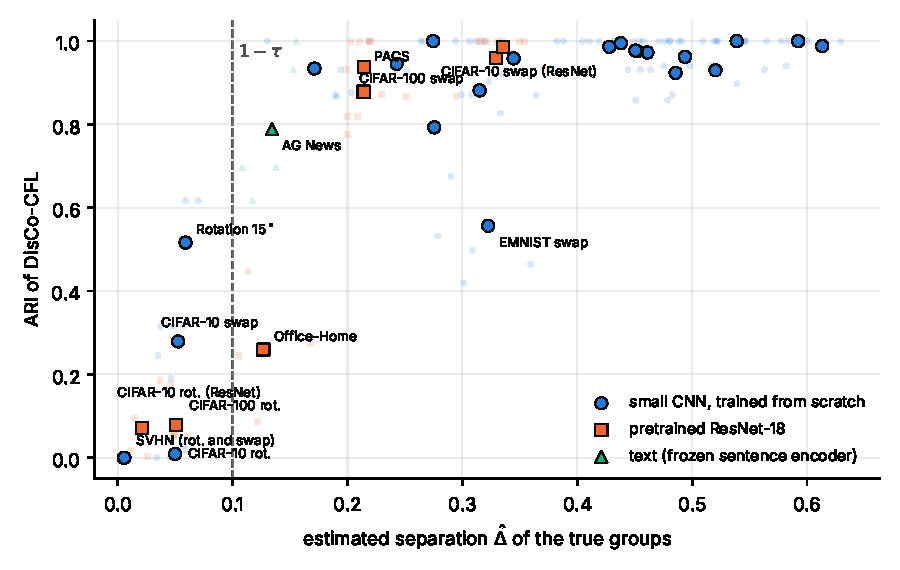
\includegraphics[width=0.85\linewidth]{../results/figures/separation.pdf}
\caption{ARI of DisCo-CFL against the estimated separation $\hat\Delta$ of the true groups, for all 31 scenarios with more than one group (large markers: means over seeds; small markers: individual runs). The dashed line is $1-\tau$, the separation that Theorem~\ref{thm:rec} requires.}\label{fig:separation}
\end{figure}

\subsection{When does DisCo-CFL succeed? Separation and the theory}\label{sec:sep}
\paragraph{Separation predicts success.} Figure~\ref{fig:separation} puts together all 31 scenarios with more than one group, from every benchmark. The estimated separation $\hat\Delta$ and the ARI of DisCo-CFL are strongly associated (Spearman $\rho=0.81$ over scenario means), and the rule ``$\hat\Delta>1-\tau$'' that Theorem~\ref{thm:rec} suggests classifies the scenarios into successes (ARI $\ge0.5$) and failures correctly in 29 of 31 cases, and in 27 of 31 at the stricter recovery level ARI $\ge0.8$ used in the hypotheses of Section~\ref{sec:extra} (there the exceptions are Office-Home, EMNIST label swaps, AG News and the 8-permutation sweep, all with $\hat\Delta>1-\tau$). We give no $p$-value: the scenarios share datasets and models and are not independent, and the association is partly mechanical, because $\hat\Delta$ is computed from the same pooled linkage that the clustering thresholds at $\tau$, which was itself chosen on four of these scenarios. The two exceptions are borderline: the $15^\circ$ rotation ($\hat\Delta=0.06$, ARI $0.52$) and Office-Home ($\hat\Delta=0.13$, ARI $0.26$). EMNIST label swaps, the one scenario where a clearly separated group is split, are counted as a success at ARI $0.56$. The failures of DisCo-CFL are therefore not erratic: they occur where the condition of the theory does not hold. The diagnostic needs the true groups and is computed after the fact; it explains the results but does not choose the reference model in advance (Section~\ref{sec:warmup}).

\begin{figure}[!htbp]
\centering
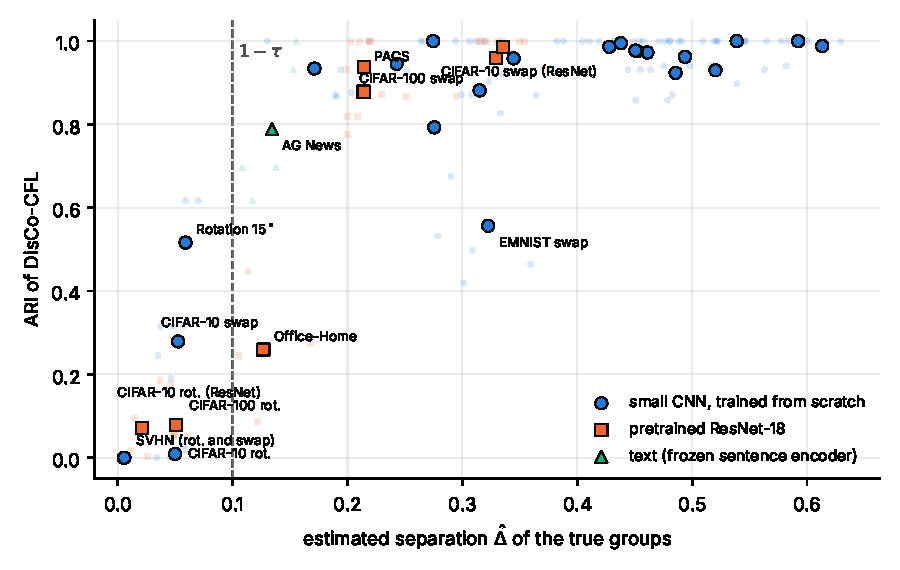
\includegraphics[width=0.85\linewidth]{../results/figures/separation.pdf}
\caption{ARI of DisCo-CFL against the estimated separation $\hat\Delta$ of the true groups, for all 31 scenarios with more than one group (large markers: means over seeds; small markers: individual runs). The dashed line is $1-\tau$, the separation that Theorem~\ref{thm:rec} requires.}\label{fig:separation}
\end{figure}


\paragraph{The results under the shrinkage covered by the theory.} The evidence condition of Theorem~\ref{thm:rec} cannot hold at the default shrinkage $\lambda=0.5$, but it can at $\lambda=0.02$ (Remark~\ref{rem:scope}(e)). We therefore reran the complete pipeline (warm-up, clustering, cluster training and evaluation) with $\lambda=0.02$ on all 24 small-CNN scenarios, with the predictions that accuracy changes by at most $0.5$ points wherever the default recovers the groups and that ARI changes by at most $0.05$ on average (Table~\ref{tab:l02} in Appendix~\ref{app:more}). Both hold. Where the default recovers the groups, mean accuracy changes by $-0.3$ to $+0.2$ points, and over all scenarios the mean absolute change in ARI is $0.014$; the largest changes are on the $15^\circ$ rotation (ARI $0.52\to0.44$) and \emph{Rotation + QS} ($0.99\to0.94$). Every success and every failure reported above is the same under the shrinkage that the theorem covers.

\paragraph{Synthetic signatures.} On synthetic signatures with known ground truth the disattenuated similarity is nearly unbiased, whereas the raw cosine is biased by up to $-0.37$, and the guarantees of Theorem~\ref{thm:rec} are reached once $h\ge64$ (Figure~\ref{fig:theory} in Appendix~\ref{app:more}).

\subsection{Choosing the warm-up without labels}\label{sec:warmup}
The failures on SVHN and CIFAR-10 come from a reference model that has not yet learned the task (Section~\ref{sec:datasets}), and 30 warm-up rounds repair SVHN label swaps. The separation diagnostic needs the true groups, however, so it cannot choose the warm-up length in practice. A first rule that stopped the warm-up when the training loss reached a plateau failed on SVHN (on one seed), because the loss is also flat \emph{before} learning starts. We therefore designed a second rule from two principles, with round constants that were not tuned. The rule, DisCo-AS, checks the federation after 10, 15, 20, 25 and 30 rounds of FedAvg and stops at the first checkpoint where (i) the training loss of the global model, reported by the clients as one scalar each, is at most $0.75\log C$ at this and at the previous checkpoint, i.e.\ the model has clearly learned something, and (ii) the DisCo-CFL partitions computed at the two checkpoints agree (ARI between them at least $0.9$); otherwise it stops at 30 rounds. No group labels are used. The predictions were that DisCo-AS changes accuracy by at most $0.5$ points where the default works (H-AS1) and improves both ARI and accuracy on SVHN and CIFAR-10 (H-AS2).

Table~\ref{tab:as} compares the rule with the default on all small-CNN scenarios, and both predictions hold. In the eleven scenarios of Fashion-MNIST, MNIST, KMNIST and EMNIST rotations where the default works, DisCo-AS stops after 15--25 rounds and changes accuracy by $-0.4$ to $+0.1$ points; the largest change in ARI is a drop from $0.98$ to $0.95$ on EMNIST rotations. On SVHN and CIFAR-10 it detects that the model has not yet learned and uses the full 30 rounds in every run, so there it coincides with DisCo-T30 (Table~\ref{tab:other}); its contribution is to make this choice without labels, not a better warm-up than 30 fixed rounds. It improves both ARI and accuracy in all four scenarios: by $11.9$ points (ARI $0.81$) on SVHN label swaps, which it now recovers in most runs, by $4.0$ points on SVHN rotations, and by $0.4$--$0.7$ points on CIFAR-10, where 30 rounds remain too few. The rule thus removes the main practical failure of the fixed warm-up on SVHN label swaps, but within a 50-round budget it cannot help when the model needs longer to separate the groups. It has been evaluated only on the small-CNN scenarios.

\begin{table}[!htbp]
\centering
\caption{Fixed 10-round warm-up (DisCo) against the label-free stable warm-up (DisCo-AS), on all small-CNN scenarios (5 seeds; sweeps 3 seeds). $\Delta$: difference in mean accuracy (points). $T_0$: warm-up length chosen by DisCo-AS. FMNIST: Fashion-MNIST; QS: quantity skew; part.: participation.}\label{tab:as}
\scriptsize
\setlength{\tabcolsep}{3pt}
\begin{tabular}{lrcccccc}
\toprule
 & & \multicolumn{3}{c}{Accuracy (\%)} & \multicolumn{2}{c}{ARI} & \\
\cmidrule(lr){3-5}\cmidrule(lr){6-7}
Scenario & $n$ & DisCo & DisCo-AS & $\Delta$ & DisCo & DisCo-AS & $T_0$ chosen (range) \\
\midrule
FMNIST rotation & 5 & 89.1 & 89.0 & -0.1 & 0.92 & 0.93 & 15 (15--15) \\
FMNIST label swap & 5 & 89.2 & 89.2 & -0.0 & 0.97 & 0.97 & 15 (15--15) \\
FMNIST rotation + QS & 5 & 88.9 & 88.8 & -0.1 & 0.99 & 0.98 & 15 (15--15) \\
FMNIST mixed + QS & 5 & 89.0 & 89.1 & +0.1 & 0.96 & 0.96 & 15 (15--15) \\
FMNIST label skew only & 5 & 94.5 & 94.5 & -0.0 & 1.00 & 1.00 & 15 (15--15) \\
FMNIST minority & 5 & 89.2 & 89.2 & -0.0 & 0.99 & 1.00 & 15 (15--15) \\
MNIST rotation & 5 & 98.1 & 98.1 & +0.0 & 1.00 & 1.00 & 15 (15--15) \\
MNIST label swap & 5 & 98.0 & 98.0 & +0.0 & 0.99 & 0.99 & 15 (15--15) \\
KMNIST rotation & 5 & 86.9 & 87.0 & +0.1 & 0.96 & 0.98 & 17 (15--20) \\
KMNIST label swap & 5 & 87.3 & 87.4 & +0.1 & 0.95 & 0.99 & 16 (15--20) \\
EMNIST rotation & 5 & 84.2 & 83.7 & -0.4 & 0.98 & 0.95 & 21 (20--25) \\
EMNIST label swap & 5 & 83.7 & 84.6 & +1.0 & 0.56 & 0.65 & 22 (15--30) \\
SVHN rotation & 5 & 69.3 & 73.3 & +4.0 & 0.00 & 0.27 & 30 (30--30) \\
SVHN label swap & 5 & 73.3 & 85.1 & +11.9 & 0.00 & 0.81 & 30 (30--30) \\
CIFAR-10 rotation & 5 & 63.5 & 63.9 & +0.4 & 0.01 & 0.10 & 30 (30--30) \\
CIFAR-10 label swap & 5 & 65.3 & 65.9 & +0.7 & 0.28 & 0.37 & 30 (30--30) \\
Rotation $15^\circ$ & 3 & 88.7 & 88.6 & -0.1 & 0.52 & 0.54 & 20 (15--30) \\
Rotation $30^\circ$ & 3 & 88.8 & 88.9 & +0.0 & 0.93 & 0.98 & 17 (15--20) \\
Rotation $45^\circ$ & 3 & 89.1 & 89.1 & -0.1 & 1.00 & 1.00 & 15 (15--15) \\
2 label permutations & 3 & 89.5 & 89.5 & -0.0 & 1.00 & 1.00 & 15 (15--15) \\
8 label permutations & 3 & 88.2 & 88.2 & +0.0 & 0.79 & 0.82 & 18 (15--25) \\
Rotation, 30\% part. & 3 & 87.1 & 86.9 & -0.2 & 0.93 & 0.93 & 15 (15--15) \\
Label swap, 30\% part. & 3 & 87.3 & 87.2 & -0.1 & 0.98 & 0.98 & 15 (15--15) \\
Rotation, 200 clients & 3 & 86.5 & 86.6 & +0.1 & 0.88 & 0.93 & 20 (20--20) \\
\bottomrule
\end{tabular}

\end{table}

\subsection{Beyond accuracy: transparency, accountability and privacy}\label{sec:fat-exp}
\paragraph{Transparency: explanations and diagnosis (H5).}
Table~\ref{tab:fat} evaluates the class-level explanations against the ground truth. For label-swap groups the divergent classes reported by the server are \emph{exactly} the swapped classes in every pair of clusters (precision, recall and exact match $1.00$), and the diagnosis ``class-specific concept shift'' is always correct. A typical explanation reads: \emph{``cluster 0 vs.\ cluster 2: class-specific concept shift on classes [4, 5, 6, 7]''}, where group 2 swaps $4\leftrightarrow5$ and $6\leftrightarrow7$. For rotations, precision is again $1.00$: no class is reported as divergent when it is not. Recall is lower ($0.75$ for rotations, $0.78$ for \emph{Mixed + QS}). The misses are classes on which the two concepts are close at the reference model, such as nearly symmetric items under a $180^\circ$ rotation. Proposition~\ref{prop:expl} guarantees fidelity only for classes with enough pooled evidence and a separation $\Delta$, so these misses are within its scope, but they make the diagnosis ``global shift'' correct for only 43\% of the rotation pairs.

\begin{table}[!htbp]
\centering
\caption{Transparency and accountability (Fashion-MNIST, 3 seeds, default settings). Certificates: share of clients with a confident certificate, and share of correctly placed clients (no conflict with any member of their cluster) among confident and among uncertain certificates.}\label{tab:fat}
\small
\begin{tabular}{lccc}
\toprule
& Rotation & Label swap & Mixed + QS \\
\midrule
\multicolumn{4}{l}{\emph{Explanations: divergent classes between clusters}}\\
precision & 1.00 & 1.00 & 1.00 \\
recall & 0.75 & 1.00 & 0.78 \\
exact set / diagnosis correct & 0.43 & 1.00 & 0.33 \\
\midrule
\multicolumn{4}{l}{\emph{Certificates}}\\
share of confident certificates & 0.76 & 0.87 & 0.77 \\
correct among confident & 0.923 & 1.000 & 1.000 \\
correct among uncertain & 0.690 & 1.000 & 1.000 \\
\midrule
\multicolumn{4}{l}{\emph{Newcomers}}\\
known concept, correctly assigned & 0.96 & 0.96 & -- \\
novel concept, flagged as novel & 1.00 & 1.00 & -- \\
\bottomrule
\end{tabular}
\end{table}

\paragraph{Accountability: certificates, audit log, newcomers (H5).}
With the jackknife standard errors of Eq.~\eqref{eq:cert}, 76--87\% of the clients receive a confident certificate. Confident certificates are correct in all cases for label swaps and \emph{Mixed + QS}, and in 92.3\% of the cases for rotations, against 69.0\% for uncertain ones. Where every client is correctly placed, the uncertain certificates are therefore conservative, as the simulation of Section~\ref{sec:outputs} predicts; under rotations they do point to the clients whose placement is in doubt. A confident certificate is informative but not a guarantee, and we report it as an empirical rate, not as a coverage probability. Newcomers that join after clustering, using the frozen reference model, are assigned to the right cluster in 96\% of the cases, and clients with a concept never seen during clustering are reported as \emph{novel} in all cases.

\paragraph{Dependence on the reference model (pre-registered).} The reference model is trained on the clients that are then clustered. To test whether the partition depends on which clients trained it, we trained it on a random half of the clients, or on all clients except those of one concept group, and clustered all clients at that model (Table~\ref{tab:refmodel} in Appendix~\ref{app:more}; six Fashion-MNIST and MNIST scenarios, 3 seeds). Both hypotheses recorded in advance hold. With a random half, ARI changes by at most $0.05$ against the full reference model, and the label-only federation stays a single cluster; clients that did not train the model are placed slightly less well than those that did (ARI $0.91$--$1.00$ against $1.00$). A group that never contributed to the reference model is still separated: at most $1.1\%$ of the conflicting pairs that involve it are merged. In these scenarios the clustering does not hinge on which clients trained the reference model, as long as the model has learned the task; this does not extend to the datasets where it has not (Section~\ref{sec:datasets}).

\paragraph{Concept drift after clustering (pre-registered).} We tested the drift procedure proposed in Section~\ref{sec:discussion} as specified in advance: after clustering, 10\% or 20\% of the clients switch to another concept group, the server recomputes all signatures at the same reference model, and every client whose similarity to its own cluster falls below $\tau$ is flagged (Table~\ref{tab:drift} in Appendix~\ref{app:more}). Every drifted client is detected (detection rate $1.00$ in all settings), but the pre-registered criterion of at most 5\% false alarms is \emph{not} met: 31--67\% of the unchanged clients are also flagged, and 38--75\% of the drifted clients are reassigned to the cluster of their new group. The cause is that the drifted clients remain members of their old cluster and pull the bottleneck similarity of their former cluster-mates below $\tau$. In an exploratory analysis that was not pre-registered, computing each client's similarity only to the members that did not drift (in practice, members that kept a confident certificate) reduces the false-alarm rate to 1--4\% with detection unchanged. Drift detection therefore works, but needs an iterative rule that first removes the clients that changed.



\paragraph{Malicious clients.} DisCo-CFL has no defence against adversarial clients, and we measured what happens when $m\in\{1,2,4\}$ of 40 clients send manipulated signatures (Table~\ref{tab:byz} in Appendix~\ref{app:more}; no hypothesis was made). Random vectors have no split-half reliability and are flagged as low-evidence or anomalous in every run; sign-flipped signatures are isolated, alone or among themselves. Neither attack harms the clustering of the honest clients (ARI $0.95$--$0.96$, at most 0.4\% conflicting merges, as without attack). A client that copies the signature of an honest client from another group, however, is always merged into that group, without being flagged: the signature carries no information that could reveal the copy. Defending against such mimicry would need authentication of the signature or secure aggregation of the clustering step, which we leave open.



\paragraph{Privacy.}
Figure~\ref{fig:dp} shows the ARI of the clustering when the signatures are released with the Gaussian mechanism of Proposition~\ref{prop:dp} ($C_{\rm clip}=0.5$, $\delta=10^{-5}$). These results measure the utility cost of noising the clustering signal only; the warm-up and the cluster training are not private (Remark~\ref{rem:dp}). As Proposition~\ref{prop:dp}(iii) predicts, the \emph{raw} cosine collapses to ARI $\approx0$ at every noise level, with 22--40 clusters: the noise attenuates all similarities. With disattenuation the clustering degrades gradually, and more data per client buys more privacy, as the $h\propto\sigma_{\rm dp}$ term predicts. Recovery is only partial, however. With 1{,}500 samples per client, ARI is $0.75$ and $0.76$ (rotation and label swap) at $\varepsilon=10$, $0.58$ and $0.65$ at $\varepsilon=4.4$, and $0.41$ and $0.55$ at $\varepsilon=2$; with 400 samples it is at most $0.43$ at any noise level we tried. Strong privacy for the clustering signal therefore needs much larger clients than our benchmarks have.

\begin{figure}[!htbp]
\centering
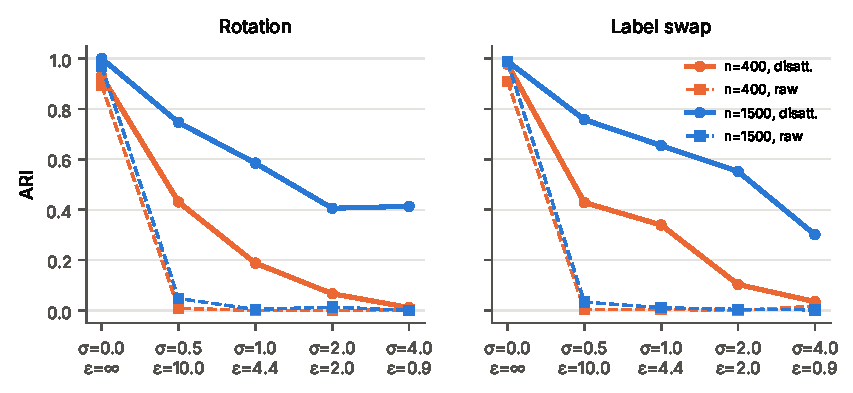
\includegraphics[width=0.85\linewidth]{../results/figures/dp.pdf}
\caption{Clustering quality under $(\varepsilon,10^{-5})$-DP signatures (3 seeds). Solid: DisCo-CFL; dashed: raw cosine. Orange: 400 samples per client; blue: 1{,}500.}\label{fig:dp}
\end{figure}

\paragraph{Class support.} The signatures reveal which classes a client holds (Section~\ref{sec:method}). Table~\ref{tab:support} (Appendix~\ref{app:more}) evaluates padding: under DP noise, every client also sends, for each class it does not hold, two independent noise vectors with the noise scale of its median class. Without padding the server knows the support exactly from the list of reported classes; even from the reliabilities alone ($R_i^c>0$) it would infer it with 77--92\% accuracy. With padding the list no longer reveals the support, but the reliabilities still do, with 63--84\% accuracy: a noise vector has a positive split-half correlation by chance in about 37\% of the cases, whereas a held class with enough data has a clearly positive one. Padding also costs clustering quality (ARI falls by up to $0.3$), because the noise classes add spurious evidence. It is therefore a weak mitigation. Hiding the support would need a mechanism that releases the support itself under DP, which we leave open.



\subsection{Calibration, sensitivity, ablation and cost}
\paragraph{Calibration and threshold (H3).}\label{sec:sens} Figure~\ref{fig:tau} varies $\tau$ on the clustering step. With disattenuation, ARI is $0.85$--$1.00$ for $\tau\in[0.85,0.95]$ in every concept-shift scenario, and the label-only scenario keeps $K=1$ up to $\tau=0.9$. With the raw cosine the useful range is narrower and higher thresholds over-split: at $\tau=0.95$ the label-only federation is split into 3 clusters and \emph{Rotation + QS} into 9.7 on average. Disattenuation therefore makes the threshold less sensitive towards high values, as H3 states. Towards low values the picture is reversed: at $\tau=0.8$ the raw cosine merges fewer groups than the disattenuated similarity (ARI $0.70$ against $0.60$ on \emph{Rotation}), because disattenuation raises all similarities, including those between groups. A calibrated scale thus shifts the useful range of $\tau$ upwards rather than widening it on both sides. The gain at the default threshold is moderate: without disattenuation (Table~\ref{tab:abl}) ARI drops by $0.04$--$0.11$ in the concept-shift scenarios and by $0.33$ in the label-only one. The sample-size study (Figure~\ref{fig:size} in Appendix~\ref{app:figs}) shows why. With clipped per-sample gradients, the raw cosine between clients of the same group is already $0.98$ on Fashion-MNIST, so there is little attenuation to correct; the disattenuated similarity is $0.99$--$1.00$. Attenuation becomes large under DP noise, where the raw cosine fails completely (Figure~\ref{fig:dp}). With very small clients (50--100 samples) both versions fail, for another reason: the groups become close at the reference model (between-group similarity $0.89$--$0.93$), i.e.\ the separation shrinks, and disattenuation does not help (ARI $0.13$--$0.63$, against $0.21$--$0.60$ for the raw cosine). Otsu's label-free threshold (Table~\ref{tab:diag}) lies at $0.76$--$0.83$ in the concept-shift scenarios. It recovers label swaps as well as $\tau=0.9$ (ARI $0.97$) but merges groups under rotations (ARI $0.58$--$0.71$). Over all scenarios (Table~\ref{tab:diag}) the comparison is two-sided. In the seven scenarios where DisCo-CFL fails (ARI below $0.5$), Otsu's threshold is better in four (e.g.\ Office-Home, $0.70$ against $0.26$; CIFAR-10 rotations with the pretrained network, $0.50$ against $0.07$), equal in the two SVHN scenarios and worse in one. In the 24 scenarios where DisCo-CFL succeeds it is lower in 19, equal in four and higher in one, and it splits single-concept federations (ARI $0$ in the label-only scenario). Its separation index $\eta$ does not distinguish successes from failures ($0.63$ for the $45^\circ$ rotation with ARI $1.00$, $0.73$ for CIFAR-10 label swaps with ARI $0.28$), so neither threshold dominates, and Otsu's rule does not replace $\tau$. The shrinkage $\lambda$ has almost no effect between $0.02$ and $1$ (Table~\ref{tab:lambda} in Appendix~\ref{app:figs}), including the values $0.02$ and $0.1$ that satisfy the condition of Corollary~\ref{cor:sc}.

\begin{figure}[!htbp]
\centering
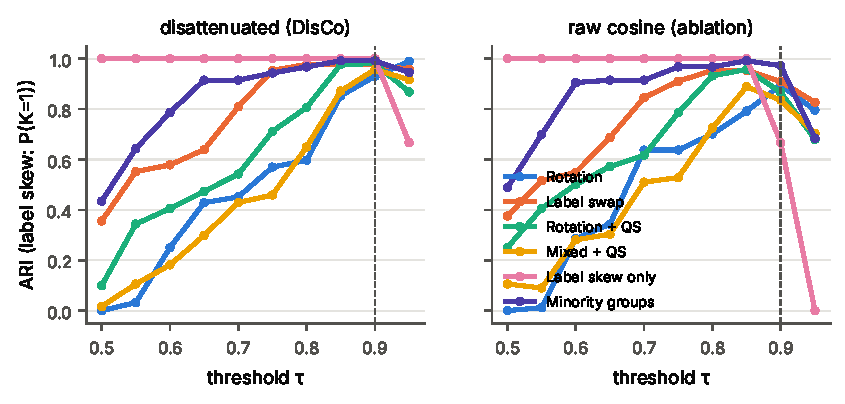
\includegraphics[width=0.85\linewidth]{../results/figures/tau_sensitivity.pdf}
\caption{Sensitivity to the threshold $\tau$ (3 seeds). The dashed line marks the default $\tau=0.9$, selected on the pilot runs (Section~\ref{sec:setup}).}\label{fig:tau}
\end{figure}

\paragraph{Edge cases.} The edge-case rules of Section~\ref{sec:method} were evaluated in three federations (Table~\ref{tab:edge} in Appendix~\ref{app:more}): the default minimum class size $m=4$ is best or close to best, the reliability floor $r_{\min}$ has no measurable effect, and extreme label skew ($\alpha=0.1$) or small clients lower ARI to about $0.7$.

\paragraph{Theory in practice.} On synthetic signatures with known ground truth the disattenuated similarity is nearly unbiased, whereas the raw cosine is biased by up to $-0.37$, and the guarantees of Theorem~\ref{thm:rec} are reached once $h\ge64$ (Figure~\ref{fig:theory} in Appendix~\ref{app:more}).

\paragraph{Ablation (H3, H4).}
Table~\ref{tab:abl} removes one component at a time. Without class conditioning (one signature per client over all its data), clients are grouped by their label mix, the failure mode reported in the survey~\citep{benali2026survey}: 18--33 clusters and a concept accuracy 19 points lower. The mean linkage averages class-specific shifts away and merges conflicting clients (11.3\% on average, ARI $0.48$ under rotations), which supports H4: the minimum over classes matters. Linkage-ordered merging over-splits label swaps and \emph{Mixed + QS}. Without disattenuation or without clipping the federation is split more often, most visibly in the label-only scenario. Without the attachment stage, a noisy client stays alone in the label-only scenario in one of the three seeds. The table uses seeds 0--2 for all rows, so the DisCo-CFL row differs slightly from the five-seed means of Table~\ref{tab:main}. The ablation supports class conditioning and the bottleneck linkage clearly; evidence-ordered merging and clipping matter only in some scenarios (linkage-ordered merging is slightly better on \emph{Rotation} and \emph{Rotation + QS}), and these two choices rest mainly on the pilot runs.

\begin{table}[!htbp]
\centering
\caption{Ablation (Fashion-MNIST, 3 seeds): ARI / number of clusters $K$ per scenario, mean conflict-merge rate (\%) and mean concept accuracy (\%) over the five scenarios.}\label{tab:abl}
\scriptsize
\setlength{\tabcolsep}{3pt}
\begin{tabular}{lccccccc}
\toprule
Variant & Rotation & Label swap & Rot.\,+\,QS & Mixed\,+\,QS & Label only & Conflict\% & Concept \\
\midrule
DisCo-CFL (full) & 0.93 / 4.3 & 0.98 / 4.0 & 0.98 / 4.3 & 0.96 / 4.0 & 1.00 / 1.0 & 0.2 & 76.9 \\
without disattenuation (raw cosine) & 0.89 / 5.0 & 0.91 / 4.7 & 0.87 / 5.3 & 0.86 / 5.0 & 0.67 / 1.3 & 0.4 & 76.0 \\
without class conditioning & 0.05 / 31.7 & 0.04 / 32.7 & 0.03 / 33.0 & 0.02 / 29.0 & 0.00 / 17.7 & 0.8 & 57.9 \\
mean instead of bottleneck linkage & 0.48 / 3.0 & 0.70 / 4.0 & 0.79 / 4.0 & 0.58 / 4.0 & 1.00 / 1.0 & 11.3 & 73.6 \\
linkage-ordered merging & 0.95 / 4.7 & 0.85 / 5.3 & 0.97 / 4.3 & 0.77 / 6.3 & 0.67 / 1.3 & 0.0 & 75.7 \\
without per-sample clipping & 0.93 / 4.3 & 1.00 / 4.0 & 0.93 / 5.0 & 0.93 / 4.3 & 0.33 / 1.7 & 0.2 & 76.6 \\
without attachment stage & 0.91 / 5.0 & 0.98 / 4.0 & 0.97 / 4.7 & 0.96 / 4.0 & 0.67 / 1.3 & 0.1 & 76.7 \\
\bottomrule
\end{tabular}
\end{table}

\paragraph{Cost and scalability.}\label{sec:cost}
Table~\ref{tab:cost} reports wall-clock time per run and the floats each client uploads for clustering. Each DisCo-CFL client uploads its signature \emph{once}, $2p|S_i|\le2pC\approx2.0\times10^4$ floats with $p=1024$ ($1.7$--$2.0\times10^4$ on average in Table~\ref{tab:cost}), independent of the model dimension $d$ (46{,}730 for the small CNN, 8.4M for the ResNet-18 block). FL+HC and StoCFL upload $d$-dimensional updates or gradients for clustering, IFCA downloads $K$ models per client in every round, and FedCCFA exchanges classifiers and class anchors in every round. A DisCo-CFL run takes about as long as a FedAvg run (the times come from shared machines, so differences below about 20\% are noise; FedAvg-FT appears faster than FedAvg on the realistic benchmarks for this reason); StoCFL takes about twice as long because it trains two models per round. Computing the signature takes about 0.09\,s per client on one CPU core, and server-side clustering 0.09\,s for 40 clients and 6\,s for 320 clients. In the clustering-only scalability study, which uses 200 samples per client, ARI is $0.59$--$0.82$ for 40 to 320 clients. With 200 clients in the full pipeline (Table~\ref{tab:sweeps}) ARI is $0.88$ and accuracy is within $0.7$ points of the Oracle. The scalability study uses one seed per size and its ARI is not monotone in the number of clients, so it measures time rather than recovery.

\begin{table}[!htbp]
\centering
\caption{Cost per run: mean wall-clock time (minutes; one CPU core for the small CNN, one GPU for the realistic benchmarks) and floats uploaded per client for the clustering signal.}\label{tab:cost}
{\scriptsize
\begin{tabular}{l c c c}
\toprule
Method & Time, small-CNN main (min) & Time, realistic (min) & Upload floats / client \\
\midrule
DisCo & 6.9 & 1.4 & 1.4e4 \\
DisCo-noAttach & 6.9 & 1.5 & 1.5e4 \\
FedAvg & 7.1 & 1.5 & 0 \\
Local & 6.9 & 1.4 & 0 \\
FedAvg-FT & 7.6 & 1.2 & 0 \\
IFCA & 11.0 & 2.8 & 0 \\
FeSEM & 7.7 & 1.6 & 0 \\
MTCFL & 6.1 & 1.3 & 0 \\
FL+HC & 7.6 & 1.6 & 1.7e6 \\
PACFL & 7.5 & 1.5 & 2.3e3 \\
StoCFL & 13.9 & 3.2 & 1.8e6 \\
StoCFL-W & 12.5 & 4.4 & 1.9e5 \\
FedCCFA & 5.2 & 3.7 & 3.8e5 \\
FedDAG-C & 7.9 & 1.5 & 4.8e4 \\
Oracle & 7.2 & 1.4 & 0 \\
DisCo-linkorder & 6.3 & -- & 1.2e4 \\
DisCo-mean & 6.0 & -- & 1.2e4 \\
DisCo-noClass & 6.0 & -- & 2.0e3 \\
DisCo-noClip & 5.9 & -- & 1.2e4 \\
DisCo-noDisatt & 6.0 & -- & 1.2e4 \\
\bottomrule
\end{tabular}
}

\end{table}

